\documentclass[oneside,a4paper,12pt]{book}
\usepackage{subcaption}
\usepackage[lmargin=2.8cm, rmargin=2.8cm, tmargin=3.3cm, bmargin=3.3cm]{geometry}
\linespread{1.1}
\setlength{\parskip}{1ex plus 0.5ex minus 0.2ex}


\usepackage[utf8]{inputenc}
\usepackage[spanish]{babel} % espanol
\usepackage{multirow} % Para las tablas

\usepackage{graphicx}%para imagenes
\graphicspath{ {img/} }
\usepackage{url}

\usepackage{varwidth} % cajas

\title{WebRTC Drone}
\author{Iván Rodríguez-Bobada Martín}

\usepackage{enumerate} % enumerados
\usepackage{listings}
\usepackage{color}
\definecolor{lightgray}{rgb}{.9,.9,.9}
\definecolor{darkgray}{rgb}{.4,.4,.4}
\definecolor{purple}{rgb}{0.65, 0.12, 0.82}


\lstdefinelanguage{JavaScript}{
  keywords={typeof, new, true, false, catch, function, return, null, catch, switch, var, if, in, while, do, else, case, break},
  keywordstyle=\color{blue}\bfseries,
  ndkeywords={class, export, boolean, throw, implements, import, this},
  ndkeywordstyle=\color{darkgray}\bfseries,
  identifierstyle=\color{black},
  sensitive=false,
  comment=[l]{//},
  morecomment=[s]{/*}{*/},
  commentstyle=\color{purple}\ttfamily,
  stringstyle=\color{red}\ttfamily,
  morestring=[b]',
  morestring=[b]"
}

\renewcommand{\lstlistingname}{Listado} % Cambiar pie de pagina de ingles a español

\lstset{
   language=JavaScript,
   backgroundcolor=\color{white},
   extendedchars=true,
   basicstyle=\footnotesize\ttfamily,
   showstringspaces=false,
   showspaces=false,
   frame=single,
   numbers=left,
   numberstyle=\footnotesize,
   numbersep=9pt,
   tabsize=2,
   breaklines=true,
   showtabs=false,
   captionpos=b
}






\begin{document}

\thispagestyle{empty}

\vspace{2cm}

\begin{figure}[htb]
\centerline{\resizebox{.60\textwidth}{!}{
\includegraphics{img/logo-urjc}}}
\end{figure}

\vspace{8mm}
\begin{center}
{\Large {\bf Grado en Ingeniería en Sistemas Audiovisuales y Multimedia}}
\vspace{8mm}

{\large Escuela Técnica Superior de Ingeniería de Telecomunicación}
\vspace{8mm}

{\large Curso académico 2015-2016}

\vspace{1.0cm}

{\large {\bf Trabajo Fin de Grado}} 

\vspace{2cm}
{\Huge {Manejo de un drone con WebRTC y JdeRobot}}

\end{center}

\vspace{4cm}
\makebox[11cm][r]{
\begin{tabular}{ll}
{\bf Autor}: & Iván Rodríguez-Bobada Martín \\
{\bf Tutor}:& José María Cañas Plaza \\
\end{tabular} 
}

\vspace{0.5cm}
\begin{center}
\large{Madrid 2015}
\end{center}



\clearpage
\thispagestyle{empty}

\vspace{5cm}
\makebox[15cm][r]{
\begin{tabular}{ll}
&\emph{A mis padres y hermanos,}\\
&\emph{que siempre han estado a mi lado,}\\
&\emph{y siempre lo estarán.}\\
&\\
&\emph{Y a mis amigos, por ser }\\
&\emph{verdaderamente mis amigos.}\\
&\\
&\emph{Gracias.}
\\
\end{tabular}
}

\let\OLDthebibliography=\thebibliography
\def\thebibliography#1{\OLDthebibliography{#1}%
  \addcontentsline{toc}{chapter}{\bibname}}

\tableofcontents
\listoffigures


\chapter{Introducción}

El proyecto que explica esta memoria se encuadra dentro del manejo, control, recogida y procesado de datos de sensores y actuadores de un drone a distancia. El drone es un vehículo aéreo no tripulado al que podemos definir dentro de la robótica aérea. En las siguientes páginas se dará unas pinceladas sobre la robótica, su historia y uso actual. También hablaremos sobre los sistemas actuales de control y manejo de drones, y para finalizar daremos una visión global sobre las tecnologías existentes dentro de las Comunicaciones en Tiempo Real (RTC, Real Time Communications).\\

\section{Robótica aérea}

Robótica es la rama de la ingeniería mecánica, ingeniería eléctrica, ingeniería electrónica y ciencia de la computación que se ocupa del diseño, construcción, operación, disposición estructural, manufactura y aplicación de los robots. Estos robots están diseñados para realizar tareas o trabajos que los humanos no podemos, por lo que requieren de cierta inteligencia. Las ciencias y tecnologías de las que depende son: el álgebra, los autómatas programables, las máquinas de estados, la mecánica o la informática.\\

Es una rama que no solo ha conseguido mediante el diseño y evolución grandes avances no solo en tareas que realizaban con anterioridad personas, sino ademas en otras que suponen una gran dificultad para ser realizadas por estas ya sea por su complejidad, como ensamblar elementos milimétricos en placas bases, o por realizarse en entornos peligrosos. Por otro lado también se han desarrollado robots domésticos para hacer nuestro día a día mas sencillo.\\

Entre los componentes \emph{hardware} que componen un robot se encuentran las fuentes de alimentación, para dotar de autonomía a los robots; sensores y actuadores, que se asemejan a los órganos sensoriales humanos y que sirven para obtener información del entorno que les rodea como temperatura u objetos próximos e interactuar con ellos; memoria, microprocesadores y dispositivos de comunicación, que es la electrónica que se comunica con el dispositivo remoto y permite gobernar los movimientos del robot.\\

Por otro lado tenemos el software, que es quien da la inteligencia al robot para llevar a cabo las funciones para las que fue diseñado.\\


La rama de la robótica aérea lleva experimentando desde hace varios años un auge espectacular. A este tipo de robots se les conoce también como Vehículo Aéreo No Tripulado ó UAV (\emph{Unmanned Aerial Vehicle}), y de una manera mas coloquial también como \emph{drones}. Se trata de aeronaves con capacidad de volar sin la presencia de un piloto a bordo que lo controle. Algunos de estos drones tienen la capacidad de volar de manera autónoma, aunque lo más común es que haya un piloto u operador teleoperandolo desde tierra.\\

\subsection{Clasificación y usos}

Podemos encontrar varios tipos de drones atendiendo a su forma y componentes materiales. Los UAV de ala fija son similares a pequeños aviones y despegan y aterrizan del mismo modo. Estos son capaces de alcanzar altas velocidades. Un ejemplo es el UAV MAVinci. Otro tipo es el de fuselaje sustentador, el cual carece de alas y se sirve del propio cuerpo para producir la fuerza de sustentación que le permite volar. Los de ala rotatoria se asemejan a los helicópteros. Suelen tener cuatro o más motores (cuadricópteros, octocópteros, etc). Tienen la ventaja de poder permanecer cernidos en un punto fijo. Ejemplos de cuadricópteros son el Phantom 4 de DJI y el ArDrone 2.0 de Parrot.\\

En la actualidad los UAV tienen utilidad en múltiples campos. Algunos de ellos son los siguientes:

\begin{itemize}
 \item \textbf{Militares.} Blancos móviles aéreos, reconocimiento de terreno y combate, entre otras tareas. 
 \item \textbf{Vigilancia.} Seguridad en hogares, vigilancia de autopistas, costas, etc. 
 \item \textbf{Inspección y reparaciones.} Fotografiar torres eléctricas, oleoductos, presas, gaseoductos, molinos eólicos, puentes, plataformas petrolíferas, etc, con el objetivo de vigilar o buscar daños que deban repararse.
 \item \textbf{Filmación.} Grabación de vídeo para retransmisiones deportivas, anuncios o escenas de cine difíciles de grabar con cámaras convencionales.
 \item \textbf{Sondas de investigación.} Es posible enviar UAV para obtener datos a partir de sus sensores o tomar muestras de partículas, microorganismos, etc. Por ejemplo, se han realizado estudios de huracanes por medio de medidas de presión y temperatura tomadas por UAV enviados al huracán.
 \item \textbf{Rescates.} Es más eficiente para rescatar personas que hayan sufrido accidentes en el mar, montañas, u otras zonas de difícil acceso, o bien víctimas de desastres naturales, contar con la ayuda de UAV que faciliten la localización de supervivientes.
 \item \textbf{Detección de incendios.} Otra utilidad es la detección de focos de fuego, por ejemplo en incendios forestales. En general son útiles para la conservación de reservas naturales o zonas protegidas.
 \item \textbf{Agricultura de precisión}. A través del uso de UAV conseguimos un estudio de las parcelas agrícolas más detallado y preciso, de manera que pueden aplicarse tratamientos de manera localizada. Permite reducir constes, mejorar la rentabilidad de los cultivos y disminuye el impacto ambiental al poder aplicarse productos agroquímicos directamente y exclusivamente a las zonas afectada
\end{itemize}


\subsection{Cuadricópteros}\label{sec:quadrotors}

Dentro de todos los tipos diferentes de vehículos UAV vamos a centrarnos en los cuadricópteros, y aunque no es necesario es conveniente que hablemos sobre la física que hace posible el vuelo de estos robots.\\

Un cuadricóptero utiliza los principios básicos de un helicóptero, utilizando cuatro rotores en vez uno. Estos rotores se acoplan a un esqueleto, el cual puede tener forma de 'x' o de '+'. Con la primera configuración tendríamos 2 motores delanteros y dos traseros (derecho e izquierdo), mientras que con la segunda configuración habría uno delantero, uno trasero y uno en cada lado. \\

Un problema que tienen que afrontar los helicópteros de un solo rotor, es que este produce una fuerza de torsión en el sentido de giro, por lo que es necesario otro rotor más pequeño perpendicular al principal para producir otra fuerza de sustentación que se oponga a la torsión y que el helicóptero no esté continuamente dando vueltas en torno a su eje vertical. En el caso de los cuadricópteros, al disponer de varios rotores, la solución a este mismo problema hacer que el giro de las hélices de una misma extremidad sea opuesto al giro de las de la otra extremidad, de forma que las torsiones se anulen.\\

Dirigir y controlar el movimiento del vehículo se consigue variando la velocidad relativa de cada rotor para cambiar el empuje y el par motor de cada uno de ellos.\\

Las hélices de los rotores, al girar, producen una fuerza de empuje hacia arriba llamada sustentación que es la que hace que se eleve el aparato. Esta fuerza es perpendicular a la velocidad del fluido relativa a la hélice y está contenida en el plano definido por la misma velocidad y la normal a la superficie de la hélice. Para que el drone despegue, la suma de fuerzas provocadas por cada rotor debe superar su peso. Una vez en el aire, si la suma de fuerzas es igual al peso, el drone permanecerá en una altitud fija o cernido (\emph{hovering}). Para aterrizar, o desplazarse hacia abajo, es necesario hacer que la fuerza resultante sea algo menor que la del peso.\\


\begin{figure}[h]
\centering
  \begin{subfigure}[]{60mm}
    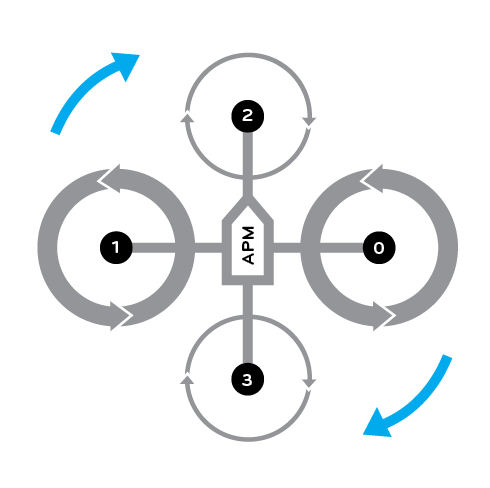
\includegraphics[width=60mm]{quadrotor-rotating}
    \caption{Giro a la derecha.} 
  \end{subfigure}
  \hspace{5pt}
  \begin{subfigure}[]{60mm}
    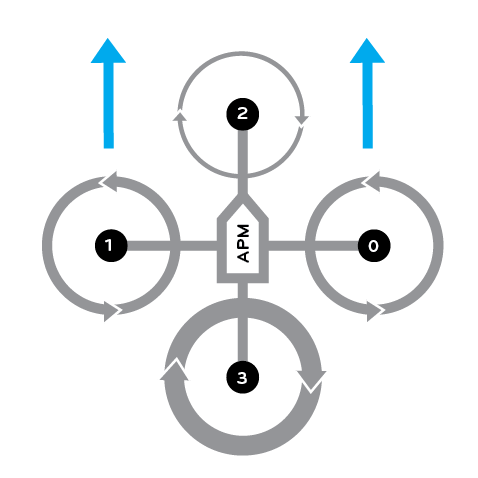
\includegraphics[width=60mm]{quadrotor-forward}
    \caption{Movimiento hacia delante.}
  \end{subfigure}
  \caption{Distintas configuraciones de los motores del cuadricóptero para desplazarse.}\label{fig:quadrotor_movements}
\end{figure}



Para provocar un giro en sentido horario será preciso aumentar la potencia en los rotores con el sentido contrario, al mismo tiempo que se reduce proporcionalmente la potencia de los otros dos para que la fuerza de sustentación siga constante, ya que en caso contrario el robot se desplazaría en su eje \emph{z}.\\


El movimiento hacia delante-atrás o hacia la derecha-izquierda se consigue disminuyendo la potencia de los rotores que estén en el lado hacia el cual se deba desplazar y aumentando los del lado contrario en igual proporción si el drone debe permanecer a una altura fija. Es decir, para movernos hacia la derecha habrá que disminuir la potencia de los rotores derechos y aumentar la de los izquierdos, de forma que el drone se incline hacia la derecha y la fuerza de sustentación tenga una componente horizontal no nula.\\


\subsection{Aplicaciones hoy en día}

Debido al auge de los cuadricópteros en los últimos tiempos se han desarrollado proyectos con los cuadricópteros como elemento principal muy interesantes unas y muy eficaces a la hora de resolver ciertos problemas otras.\\

\subsubsection{Lily Drone} 

Lily\footnote{https://www.lily.camera} es un cuadricóptero de reducidas dimensiones y peso (1.3kg) el cuál va equipado con una cámara capaz de grabar vídeo hasta resolución de alta definición a 1080p y 120fps.\\

Lo más llamativo de este drone no son sus capacidades de vuelo ya que sólo nos permite vuelos de hasta 15 metros de altura y unos 40km/h de velocidad, si no que simplemente llevando un dispositivo de detección de reducidas dimensiones (28g), lo enciendes y él, sin necesidad de configuración, te detecta y sigue todos tus movimientos mientras a la vez te está grabando. Los vuelos son de unos 20 minutos de duración, y el drone es resistente al agua, por lo que puedes usarlo prácticamente en cualquier tipo de situación.\\


\begin{figure}[htb]
\centering
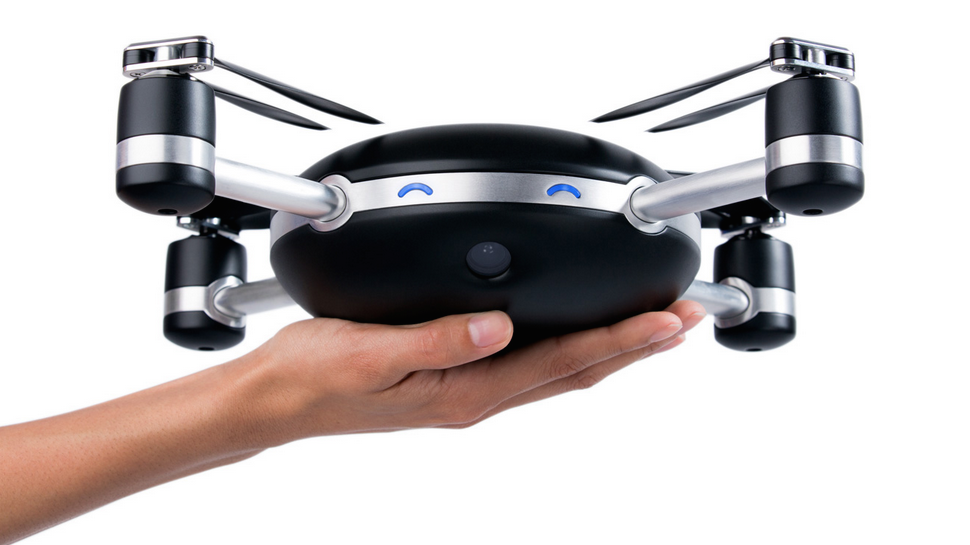
\includegraphics[width=0.7\textwidth]{lily1}
\end{figure}

\begin{figure}[htb]
\centering
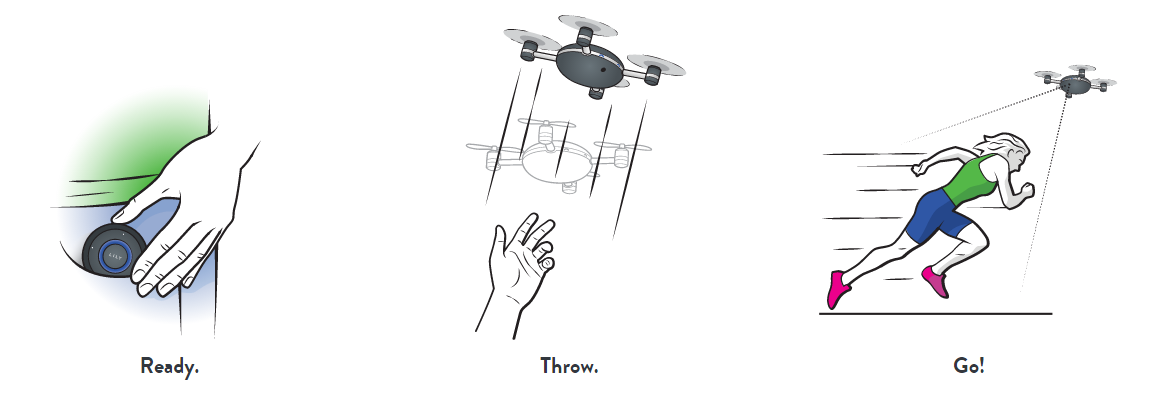
\includegraphics[width=1\textwidth]{lily2}
\caption{Lily (a) y funcionamiento en 3 pasos (b).}
\label{fig:lily}
\end{figure}


\subsubsection{Hemav, Agricultura de precisión.}

La empresa Hemav\footnote{http://hemav.com} ofrece entre otros servicios agricultura de precisión a través del vuelos con cuadricópteros. Utilizan sensores multiespaciales y/o térmicos para generar mapas aéreos mediante vuelos autónomos que su suministran información relevante para la toma de decisiones.\\

Posteriormente esa información es analizada estadísticamente para generar patrones de estados, similitudes de terreno, detección de patologías, etc, con los que finalmente se genera un informe con las conclusiones especificas.\\

\begin{figure}[h]
\centering
  \begin{subfigure}[]{60mm}
    \includegraphics[width=60mm]{hemav2}
    \caption{Hemav.} 
  \end{subfigure}
  \hspace{5pt}
  \begin{subfigure}[]{60mm}
    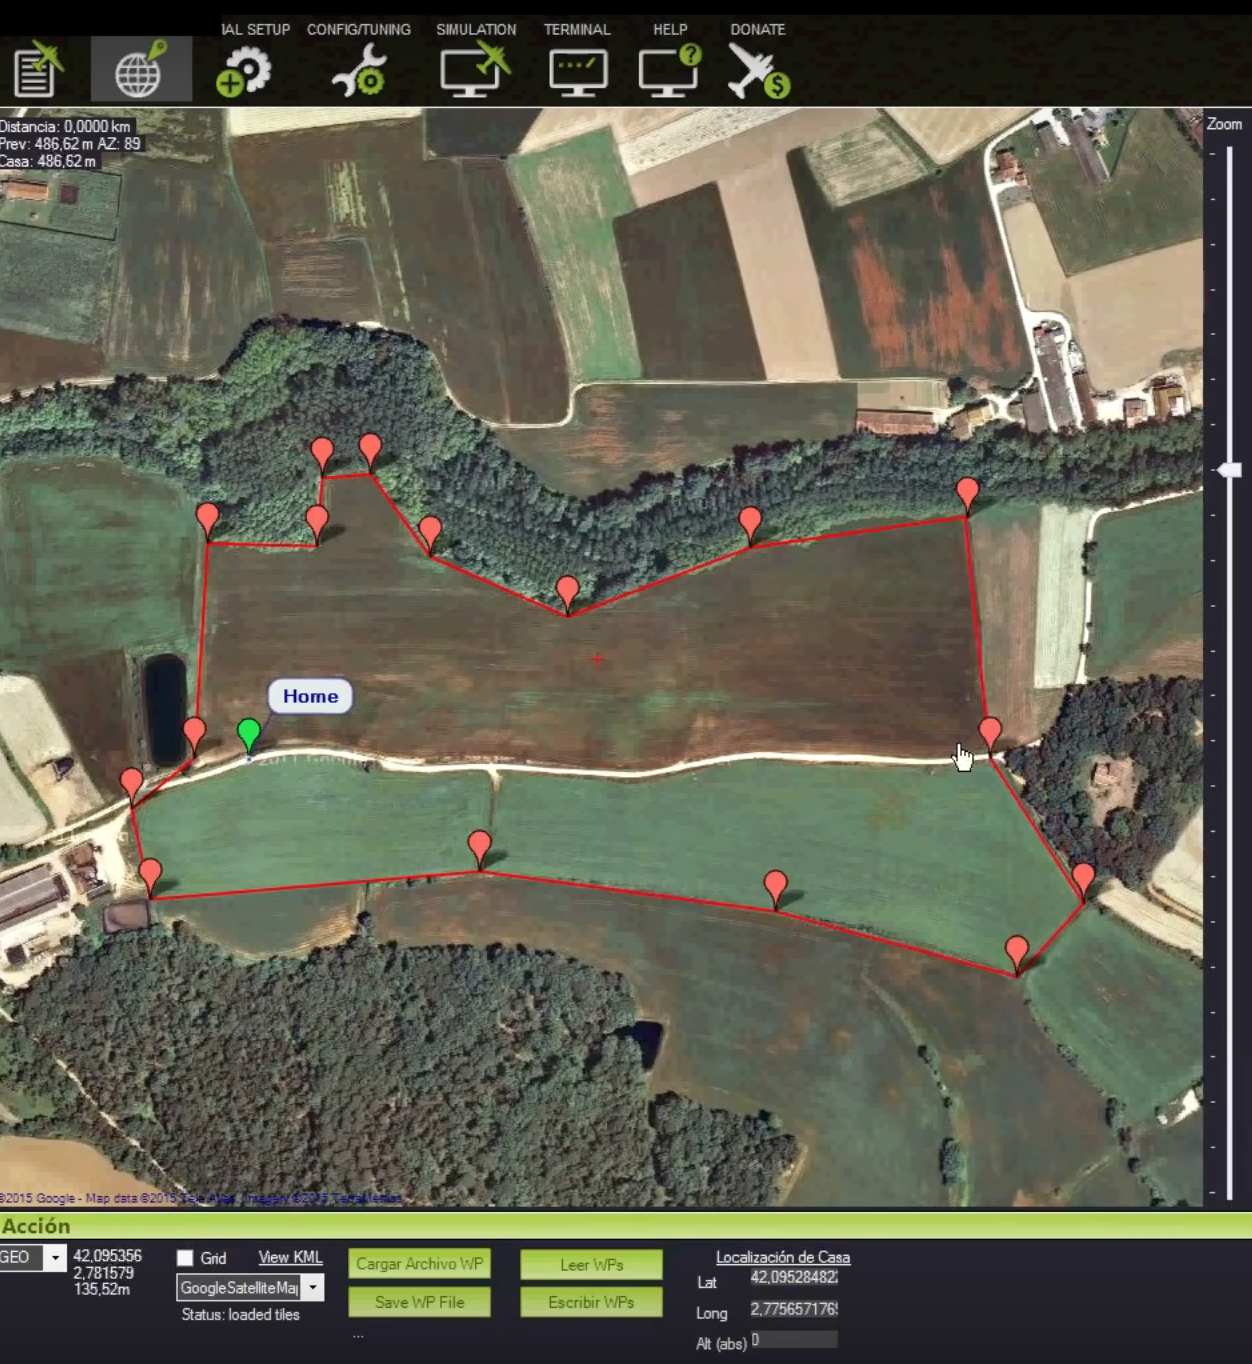
\includegraphics[width=60mm]{hemav1}
    \caption{Finca acotada para el vuelo autónomo.}
  \end{subfigure}
  \label{fig:hemav}
\end{figure}


\subsubsection{Entrega de paquetes con drones.}

La entrega de paqueteria usando vehiculos aéreos no tripulados es el futuro, aunque ya muy presente en cuanto a la entrega de paquetes a domicilio se refiere. Las funcionalidades son muy numerosas, desde entrega de comida o compras realizadas a domicilio, hasta entrega de medicamentos o comida a personas en apuros o situaciones peligrosas.\\

Empresas como Amazon con su proyecto \emph{Prime Air} (figura \ref{fig:amazon}), DHL, Google con \emph{Project Wing} o la NASA están trabajando para desarrollar sus propios sistemas de entrega de paquetería a domicilio a través de drones.\\

\begin{figure}[htb]
\centering
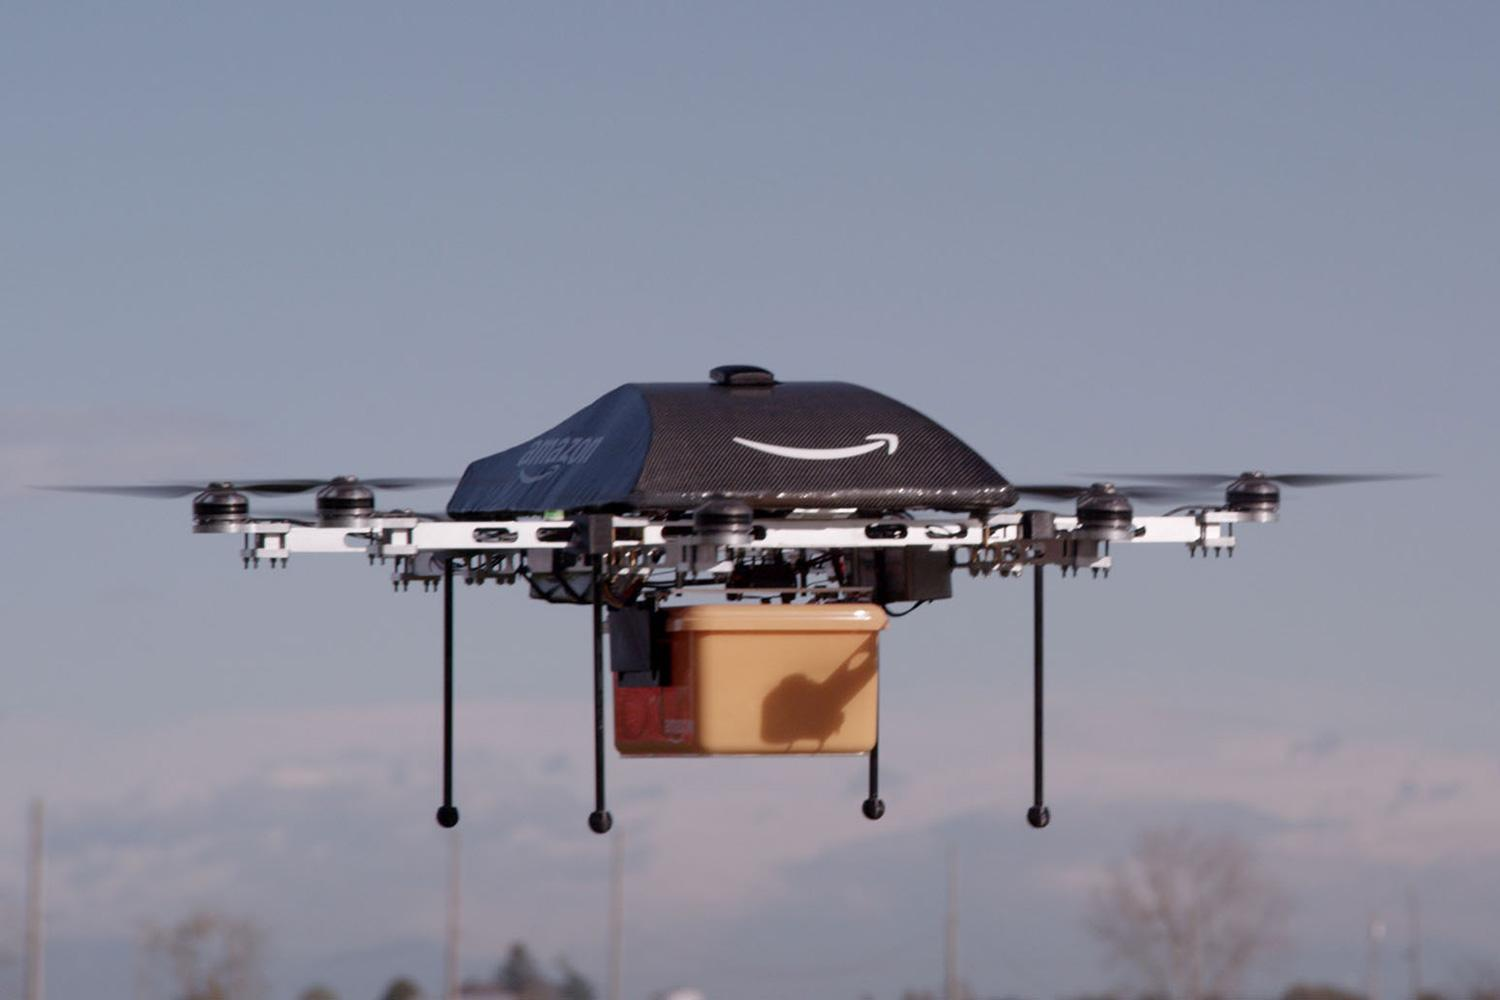
\includegraphics[width=0.9\textwidth]{amazon}
\caption{Amazon Prime Air}
\label{fig:amazon}
\end{figure}

\subsubsection{Drones en salvamento marítimo.}

La Agencia de Medios de Vodafone (MEC) y los expertos de Trabajos con Dron\footnote{trabajoscondrone.com} (TcD) han desarrollado un proyecto de drones socorristas. Estos reducen hasta en tres vees el tiempo en llegar al ugar del accidente con respecto al socorrista tradicional.\\

En caso de incidente, el socorrista-piloto conducirá el drone con el mando de radiocontrol ayudándose de la cámara que lleva a bordo, cuando llega al punto de incidencia lanzara un par de flotadores a los que se pueden agarrar hasta que llegue el equipo de salvamento.\\

 \begin{figure}[htb]
\centering
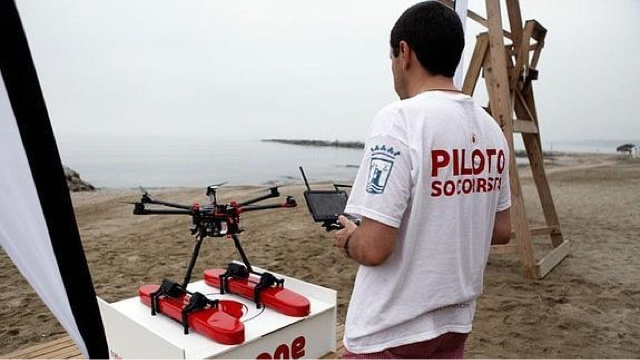
\includegraphics[width=0.9\textwidth]{socorrista}
\caption{Drone de Salvamento Marítimo}
\label{fig:socorrista}
\end{figure}

\subsubsection{Drones en el cine y televisión.}

Hace tiempo que los robots teledirigidos participan en los rodajes, pero solo recientemente han pasado a de tener un papel secundario a convertirse en protagonistas. En la industria cinematográfica se ha añadido el uso del drone para grabar escenas que antes eran complicadas, costosas o imposibles de grabar. Han cobrado tanta importancia que hasta han creado certámenes como el \emph{Flying Robot International Film Festival} para premiar la su uso en la grabación. Los drones nos proporcionan nuevas perspectivas en todo tipo de secuencias.\\

Peliculas como el Lobo de Wall Street, Jurassic World o Skyfall han incorporado entre sus métodos de grabación la utilización de drones. También se utilizan en el mundo de la televisión. Entre otros el famoso programa inglés \emph{Top Gear} o el documental de la BBC Planeta Tierra.

\begin{figure}[htb]
\centering
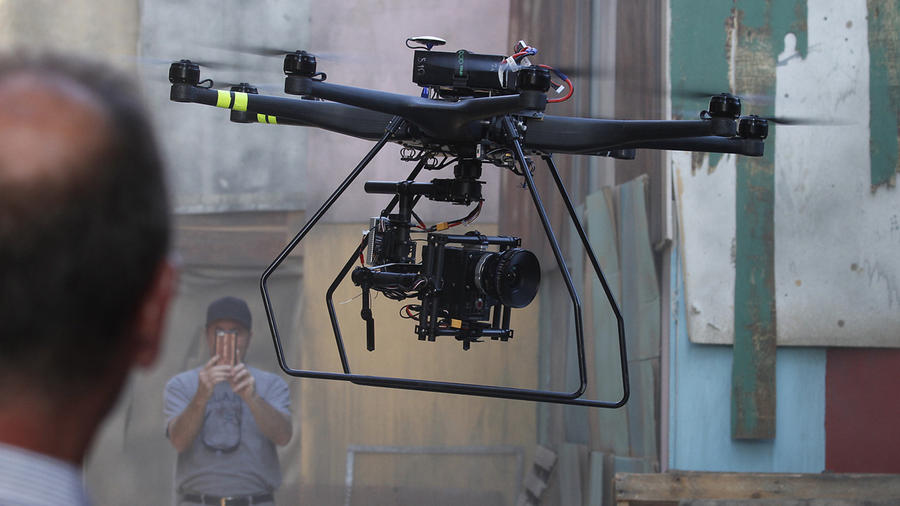
\includegraphics[width=0.9\textwidth]{dronefilm}
\caption{Uso de un drone para grabación.}
\label{fig:amazon}
\end{figure}



\subsection{Sistemas de control de drones}
\label{cap:controldrones}

Los drones pertenecen a la rama de robótica aérea, pero a su vez también son vehículos aéreos no tripulados (\emph{UAV, Unmanned  Aerial Vehicle}). Es un vehículo no tripulado, pero no autónomo, por lo que necesitan ser teleoperados desde tierra. Los sistemas actuales para ello se pueden dividir en dos grupos, los controlados mediante radiofrecuencia y los que usan sistemas alternativos.\\

\subsubsection{Radiocontrol}

Es la técnica que permite el gobierno de un objeto a distancia de manera inalámbrica mediante una emisora de control remoto. Por otra parte, a bordo del vehículo, en nuestro caso un drone, debe ir una receptora de radio control. \\

\begin{figure}[htb]
\centering
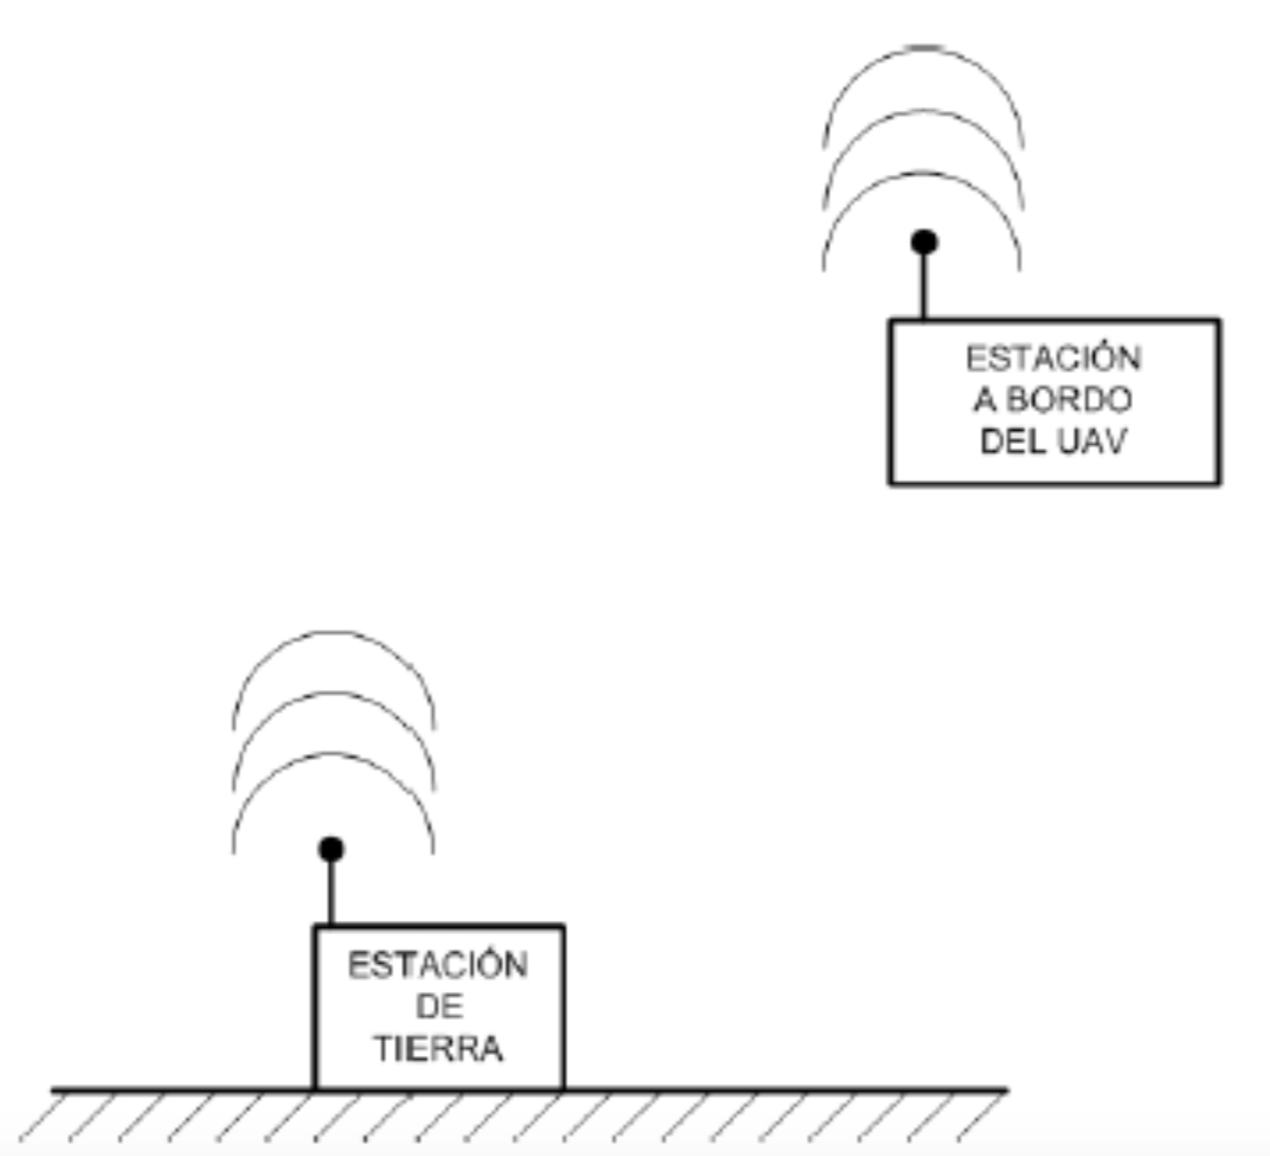
\includegraphics[width=0.8\textwidth]{radiocontrol}
\caption{Sistema RC para estaciones UAV}
\label{fig:radiocontrol}
\end{figure}


La comunicación entre receptor y transmisor se efectúa mediante radiofrecuencia, existiendo diferentes sistemas de emisión, como AM, FM o 2.4Ghz con diferentes tipo de codificación, PCM, PPM…\\

Estos sistemas tienen varias limitaciones. Una es el número de canales máximo del sistema, ya que se usa un canal para cada elemento de control disponible: elevación, giro, rotación… La segunda y posiblemente más crítica son las interferencias. Si se producen interferencias ya sea por ruido o por varios emisores trabajando en las cercanías se puede perder el control de la aeronave produciendo una posible colisión, destruir la misma o incluso dañar a personas.\\
 
\subsubsection{Sistemas alternativos}

En la actualidad a parte del radiocontrol tenemos el control a través de WiFi. Este sistema consiste en la creación de una red WiFi por parte del drone a la cual se conecta el dispositivo con el que se maneja. Este dispositivo puede ser un mando diseñado y comercializado por la propia marca o un dispositivo móvil, el cuál usa una aplicación que es la que gestiona la conexión y transferencia de datos.\\

La ventaja de estos sistemas es el ahorro de batería, ya que los transmisores y antenas WiFi necesitan de menos potencia para cubrir las mismas distancias que los sistemas tradicionales de radiocontrol. Además el ancho de banda que nos proporciona es bastante elevado y podremos transferir tanto datos como las imágenes de las cámaras HD a bordo del drone.\\

Empresas como DJI usa sistemas mixtos que consisten en teleoperar el drone vía radiocontrol, pero la gestión y visualización de la cámara se realiza mediante una conexión WiFi como la explicada anteriormente.\\
 
La empresa francesa Parrot, la cual tiene una flota de diversos modelos de drones, utiliza un sistema de red WiFi, a la cuál conectas un dispositivo móvil ya sea Android o iOS, y mediante una aplicación desarrollada por ellos se puede teleoperar el drone, así como tener otras funcionalidades como la grabación de vídeo, captura de imágenes y gestión de parámetros de vuelo como altura o velocidad máxima. En capítulos posteriores profundizaremos en este sistema implementado, ya que es el que usaremos para desarrollar el nuestro.\\



\section{Tecnologías de Comunicación en Tiempo Real}

En la actualidad  existen numerosas tecnologías de comunicación en tiempo real, pero nos centraremos en las que nos ofrecen conectividad multimedia. Primero veremos protocolos que se pueden implementar en aplicaciones de escritorio, y posteriormente veremos los protocolos web mas actuales.\\

\subsection{RTP}

\emph{RTP} son las siglas de \emph{Real-time Transport Protocol} o Protocolo de Transporte en Tiempo Real, el cuál es un protocolo para aplicaciones de escritorio y de nivel de sesión utilizado para la transmisión de información en tiempo real, como por ejemplo audio, vídeo y datos. Está desarrollado por el grupo de trabajo de transporte de audio y vídeo del IETF (\emph{Internet Engineering Task Force}). Este protocolo es la base de la industria de Voz sobre IP (\emph{VoIP}).\\

Se encapsula sobre UDP y usa un puerto de usuario para cada medio que transfiere. Admite direcciones de destino tanto \emph{unicast} como \emph{multicast}. Se encarga de enviar cualquier tipo de trama generada por cualquier algoritmo de codificación como H261, MPEG-1, MPEG-2... pero no añade ningún tipo de fiabilidad ni de calidad del servicio (\emph{QoS}). Lo único que incorpora son marcas de tiempo para evitar el tembleque o \emph{jitter} y la sincronización entre flujos en el destino y números de secuencia para detectar pérdidas en un flujo.\\

RTP trabaja junto con otros dos protocolos que lo complementan. El primero es RTCP (\emph{Real time Control Protocol}), protocolo que proporciona información de control sobre la calidad de la transmisión. Transmite paquetes periódicos asociados a cada flujo RTP que incluye los detalles sobre los participantes, si hubiese más de uno, y las estadísticas de pérdidas que permiten el control de flujo y congestión. Según estas estadistas se puede hacer codificación adaptativa para adaptarse al medio. También trabaja sobre UDP y usa un numero de puerto superior al que usa el flujo de RTP.\\

El segundo es RTSP (\emph{Real Time Streaming Protocol}), protocolo que permite realizar un control remoto de sesión de transmisión multimedia. Es un protocolo independiente del protocolo de transporte, basado en texto que permite recuperar un determinado medio de un servidor o grabar una multiconferencia.\\

La norma define también el protoclo SRTP (\emph{Secure Real-time Transport Protocol}), el cuál es una extensión del perfil de RTP para conferencias de audio y vídeo que puede usarse para proporcionar confidencialidad, autenticación de mensajes y protección de reenvío para flujos de audio y vídeo.\\


\begin{figure}[htb]
\centering
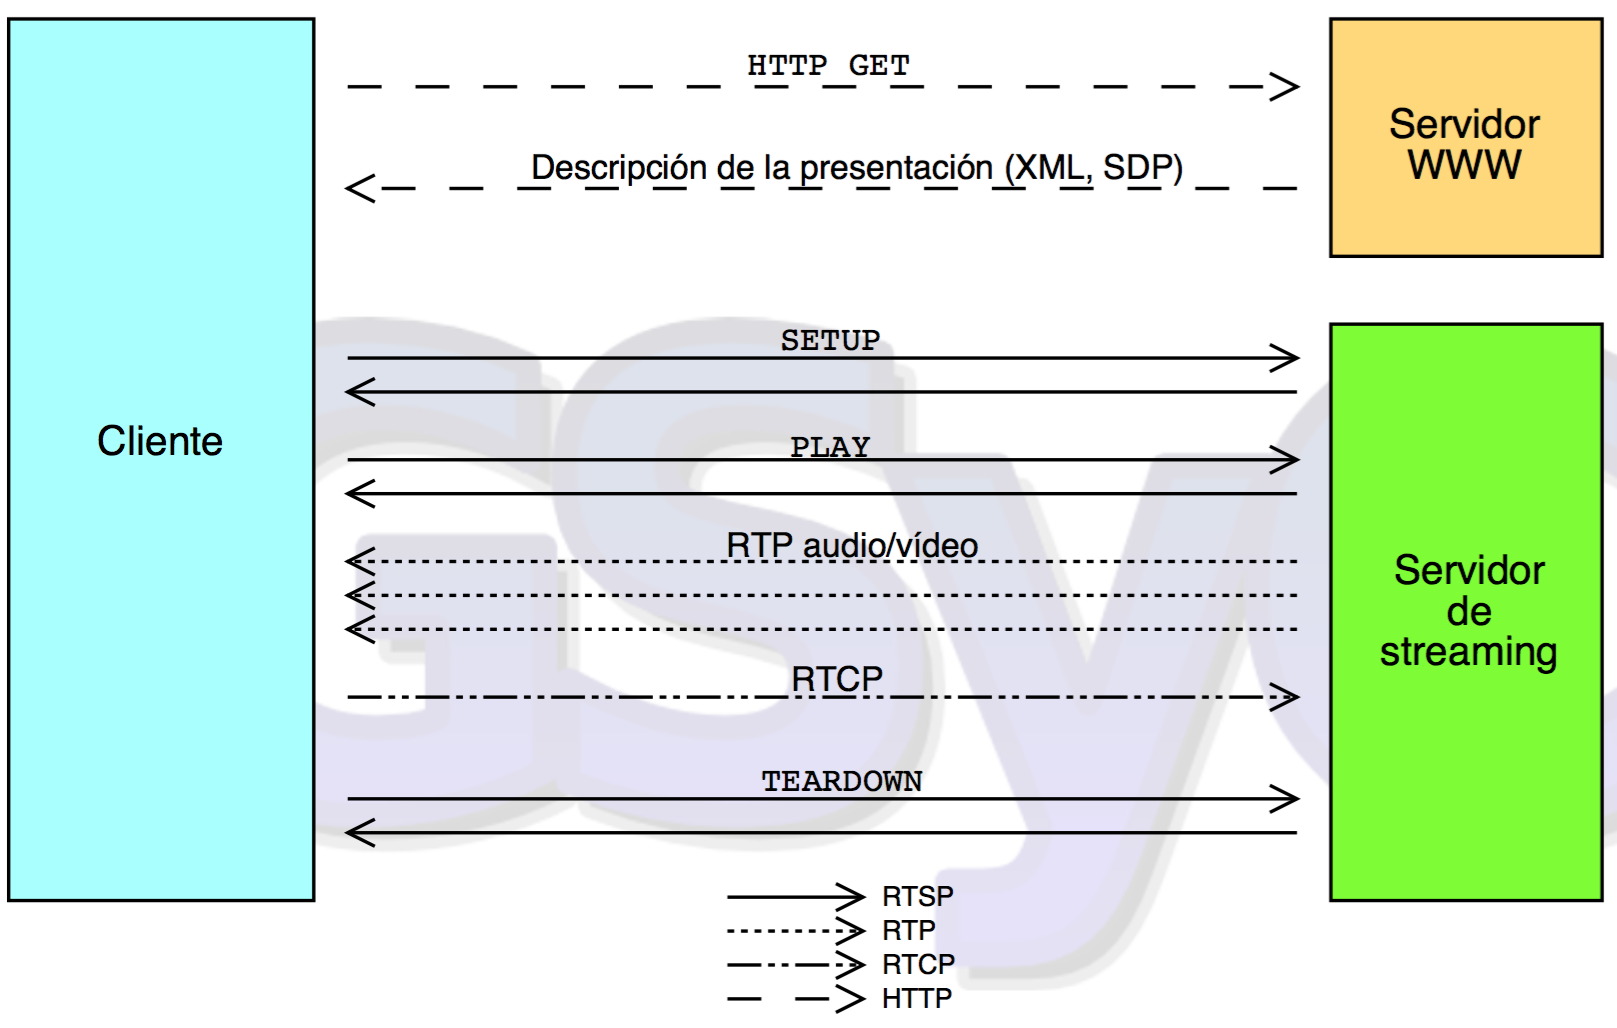
\includegraphics[width=0.8\textwidth]{rtc}
\caption{Ejemplo de conexión RTC, RTCP y RTSP}
\label{fig:rtc}
\end{figure}


\subsection{SIP}

SIP o Protocolo de Inicio de Sesiones (\emph{Session Initiation Protocol}) es un protocolo desarrollado por el grupo de trabajo MMUSIC del IETF con la intención de ser el estándar para la iniciación, modificación y finalización de sesiones interactivas de usuario donde intervienen elementos multimedia como vídeo, voz, mensajería instantánea...\\

Técnicamente no es un protocolo que transmite flujos multimedia, si no que es un protocolo de señalización cuya función es preparar el establecimiento y la terminación de sesiones multimedia entre máquinas remotas. Una de sus mas importante funciones es el intercambio de las descripciones de sesión (\emph{SDP}) de los usuarios. El concepto de sesión en este protocolo es muy amplio: una llamada entre dos, una videoconferencia, un juego interactivo entre varios usuarios...\\

Es un protocolo muy ligero. Tiene solo 6 métodos basados en texto, de manera similar a HTTP o SMTP, pero es completamente independiente del protocolo de transporte utilizado (TCP, UDP, ATM, etc). \\

Es el protocolo señalizador para el protocolo RTP explicado anteriormente. Entre otras, Ekiga, WengoPhone, MS Windows Messenger, Apple iChat AV ó Asterisk son algunas aplicaciones que utilizan SIP.\\


\begin{figure}[htb]
\centering
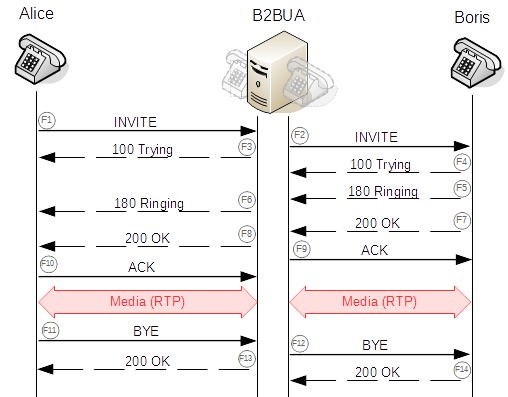
\includegraphics[width=0.8\textwidth]{sip}
\caption{Ejemplo de conexión SIP}
\label{fig:sip}
\end{figure}

En la figura \ref{fig:sip} podemos ver un ejemplo de una conexión multimedia con RTP que utiliza el protocolo SIP para establecer y finalizar la sesión entre los dos usuarios.\\

\subsection{ORTC}

\emph{Object RTC} es un proyecto de código abierto que permite la comunicación en tiempo real (\emph{RTC, Real-Time Communications}) de dispositivos móviles con servidores u otros navegadores con el simple uso de unas API's JavaScript nativas en el navegador.\\ 

El objetivo de Object RTC es permitir crear comunicaciones en tiempo real con una alta calidad en dispositivos móviles y servidores con el simple uso de JavaScript y HTML5. Es también una obligación para ORTC ser compatible con WebRTC.\\

Aunque ORTC es un proyecto respaldado por empresas de la talla de Hookflash, Microsoft o Google, por el momento no es una especificación del consorcio W3C (\emph{World Wide Web Consortium}).\\

ORTC comparte muchas similitudes con WebRTC. Como mayor diferencia tenemos que ORTC no utiliza SDP ni el protocolo de Oferta/Respuesta, en cambio utiliza los objetos 'enviador' (\emph{sender}), 'recibidor' (\emph{receiver}) y 'transporte' (\emph{transport}), los cuales tienen capacidades que describen que pueden hacer y sus parámetros que definen como están configurados. Además ORTC no está disponible nada más que en el navegador Edge de Microsoft.\\

\begin{figure}[htb]
\centering
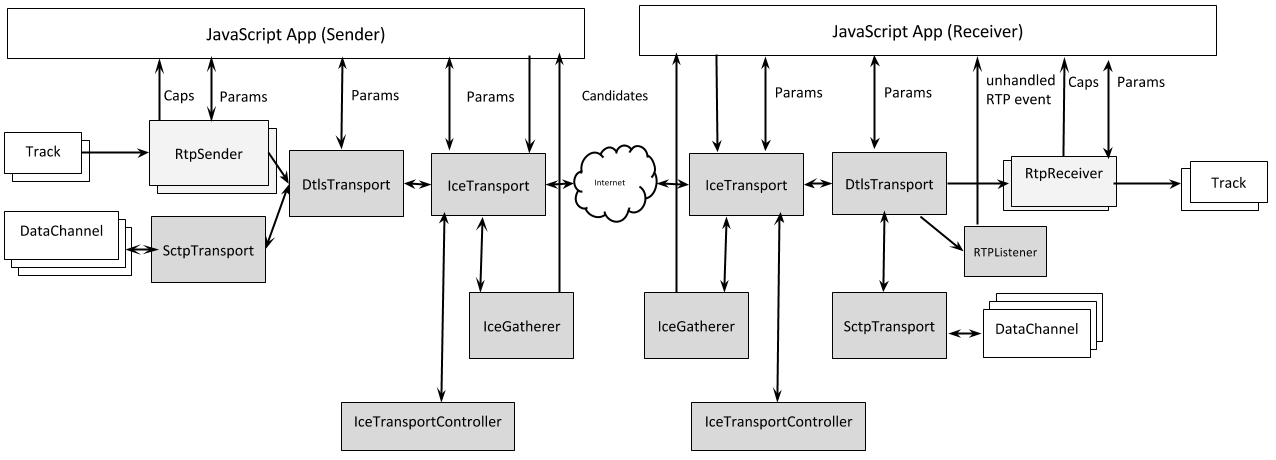
\includegraphics[width=0.9\textwidth]{ortc}
\caption{API de ORTC}
\label{fig:ortc}
\end{figure}


\subsection{WebRTC}

En mayo de 2011 Google liberó un proyecto de código abierto basado en la comunicación entre navegadores en tiempo real. El proyecto ha sido continuado estandarizando los protocolos en el IETF y las API's de JavaScript en el W3C.\\

En el consorcio W3C WebRTC es aún un borrador de un proyecto en marcha el cuál esta altamente implementado en los navegadores como Mozilla Firefox y Google Chrome. La API está basada en el trabajo previo realizado por \emph{Web Hypertext Application Technology Working Group} (WHATWG).\\

Esta tecnología nos brinda la capacidad de crear numerosas aplicaciones de comunicaciones entre navegadores, sin necesidad de servidores internos, y está llamada a ser el futuro de las comunicaciones en tiempo real.\\

\begin{figure}[htb]
\centering
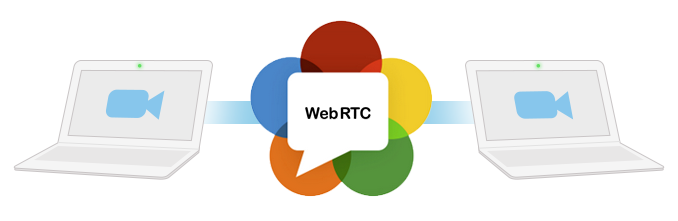
\includegraphics[width=0.9\textwidth]{webrtc}
\caption{WebRTC}
\label{fig:webrtc}
\end{figure}



\section{Motivación y antecedentes}

En estos últimos años el desarrollo de vehículos no tripulados ha tenido un avance muy significativo, sobre todo en aplicaciones de uso civil. Uno de los campos en los que más ha despuntado es en el uso para la grabación de cualquier tipo de eventos, tanto a nivel profesional como a nivel \emph{amateur}.\\

Las tecnologías web son otro campo que ha experimentado un avance enorme en los últimos años, permitiendo crear aplicaciones mas complejas y elaboradas. Estas aplicaciones a la vez de ser mas potentes se pueden implementar directamente en un navegador, sin necesidad de ningún tipo de instalación en el ordenador del cliente.\\

El fondo del proyecto consiste aunar estos dos campos. Se pretende desarrollar una aplicación web con tecnologías de última generación que permita teleoperar el drone.\\

Como base para el proyecto para desarrollar la aplicación web tenemos los siguientes proyectos, desarrollados también por alumnos de la URJC.\\

\subsection{Surveillance 4.0 (URJC)}

Surveillance 4.0 desarrollado por Daniel Castellano como su Proyecto Fin de Carrera. Esta aplicación contaba con varios sensores de distinto tipo (humedad, temperatura, gas, etc) que se conectaban inalámbricamente con un nodo central situado en una Raspberry Pi. La conexión inalámbrica se hacía mediante transmisores Zigbee con un protocolo propio llamado WHAP. El nodo central recibía los datos de los sensores y los mostraba mediante un servidor web que corría en la misma máquina. La aplicación web se desarrolló en Python usando el entorno de desarrollo web Django. En Surveillance 4.0, los valores de los sensores se guardaban en una base de datos que la aplicación web consultaba cuando era necesario. Además, esta versión incluía un streaming de vídeo utilizando el software de código abierto M-JPEG Streamer. En la figura \ref{fig:surveillance4} se puede ver la aplicación.\\

\begin{figure}[h]
\centering
  \begin{subfigure}[]{110mm}
    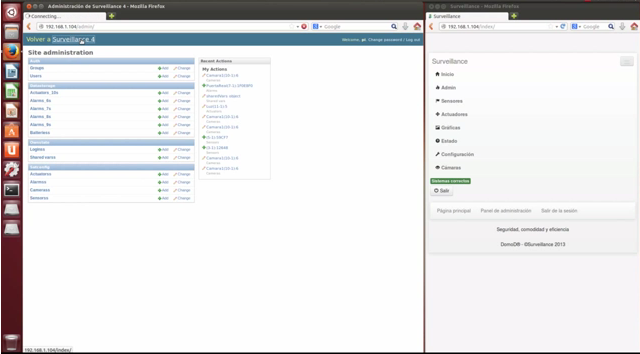
\includegraphics[width=110mm]{surveillance4}
  \end{subfigure}
  \hspace{5pt}
  \begin{subfigure}[]{110mm}
    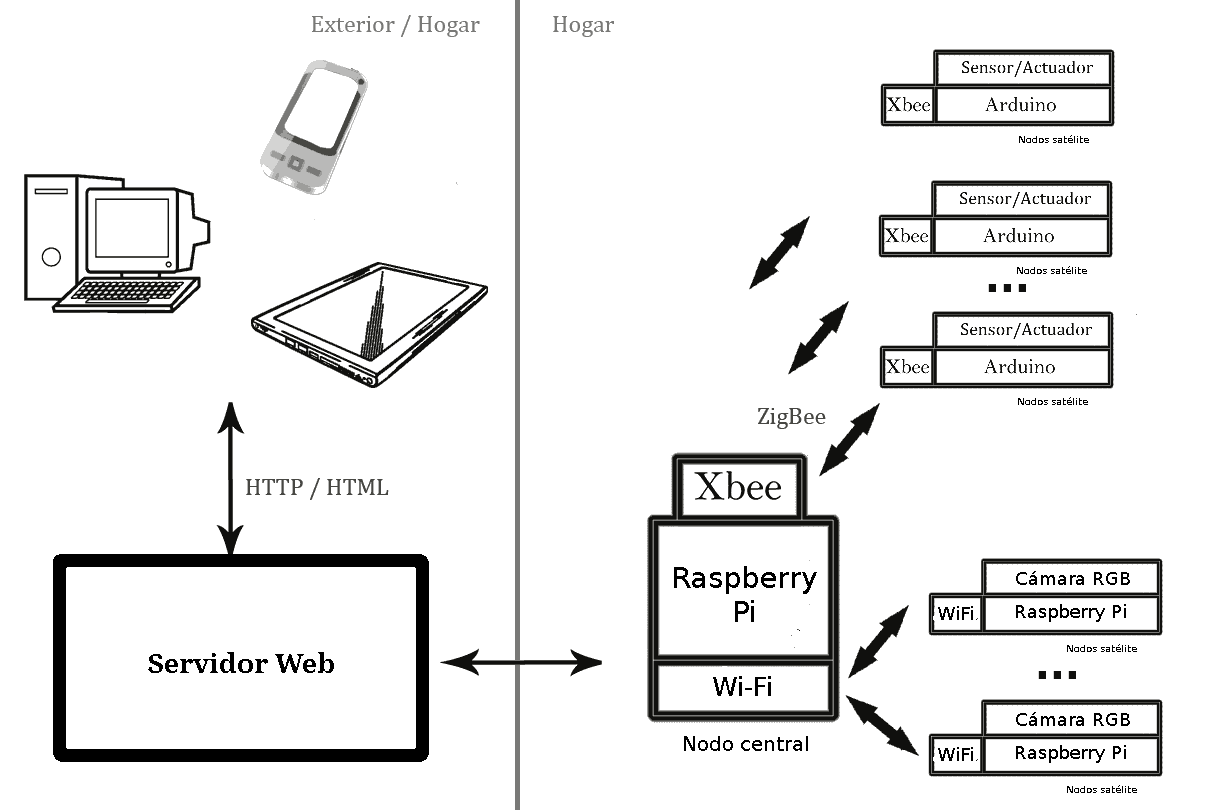
\includegraphics[width=110mm]{Esquema_s4}
  \end{subfigure}
  \caption{interfaz (a) y arquitectura (b).}\label{fig:surveillance4}
\end{figure}



\subsection{Surveillance 5.1 (URJC)}

Surveillance 5.1 desarrollado por Edgar Barrero como su Trabajo Fin de Grado. Esta aplicación obtenía un flujo de imágenes de una cámara web, un flujo de imágenes de profundidad de un sensor Kinect, además de datos de un sensor de humedad y de interaccionar con un actuador. La aplicación web se desarrolló en Ruby sobre Rails. En Surveillance 5.1, el servidor web se conectaba a los componente de JdeRobot mediante sus interfaces ICE. La aplicación web refrescaba estos datos mediante peticiones AJAX.  En la figura \ref{fig:surveillance5} se puede ver la aplicación.\\


\begin{figure}[h]
\centering
  \begin{subfigure}[]{110mm}
    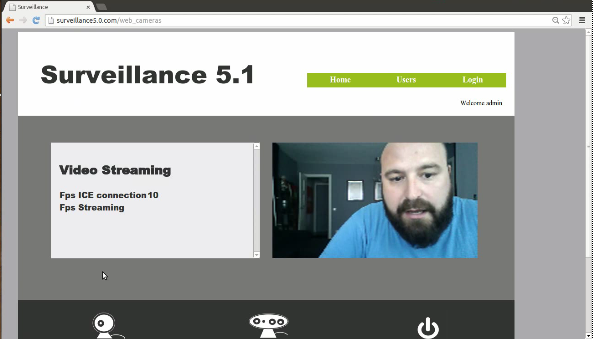
\includegraphics[width=110mm]{surveillance5}
  \end{subfigure}
  \hspace{5pt}
  \begin{subfigure}[]{110mm}
    \includegraphics[width=110mm]{esquema_s4}
  \end{subfigure}
  \caption{interfaz (a) y arquitectura (b).}\label{fig:surveillance5}
\end{figure}


\subsection{Teleoperadores y visores Web en JdeRobot}

Esta plataforma está desarrollada por Aitor Martínez como su Trabajo Fin de Grado. Está compuesta por seis clientes Web: CameraViewJS, RGBDViewerJS, KobukiViewerJS, UavViewerJS, IntrorobKobukiJS e IntrorobUavJS, los cuales son las versiones web de las herramientas homónimas desarrolladas por JdeRobot. Estas nuevas herramientas hablan directamente con los servidores desarrollados por JdeRobot para acceder a los sensores y robots, y como diferencia principal destacable no necesitan de servidores intermedios para funcionar, utilizando \emph{websockets} para establecer las conexiones necesarias.\\

\noindent Las funcionalidades de estos clientes web son: 

\begin{enumerate}

\item \emph{CameraViewJS:} Cliente web similar a la herramienta \texttt{CameraView} para visualizar imágenes procedentes del servidor \texttt{Cameraserver}. 

\item \emph{RGBDViewerJS:} Cliente web similar a la herramienta RGBDViewer para visualizar datos de color y profundidad procedentes del servidor \texttt{Openni1Server}.
  
\item \emph{KobukiViewerJS:} Teleoperador para manejar y ver los datos de los sensores de los robots Kobuki y Pioneer del laboratorio de robótica de la URJC. Versión web de \texttt{KobukiViewer}
  
  
\item \emph{UavViewerJS:} Cliente web similar a la herramienta UavViewer para teleoperar drones tanto reales como simulados y ver los datos de sus sensores.
  
  
\item \emph{IntrorobKobukiJS e IntrorobUavJS} Son dos herramientas que además de mostrar los datos sensoriales del robot y ofrecen su teleoperación, permiten insertar código que gobierna el comportamiento autónomo de robots Kobuki y drones. En la figura \ref{fig:introrobuavjs} podemos ver la herramienta IntrorobUavJS.

\end{enumerate}

\begin{figure}[htb]
\centering
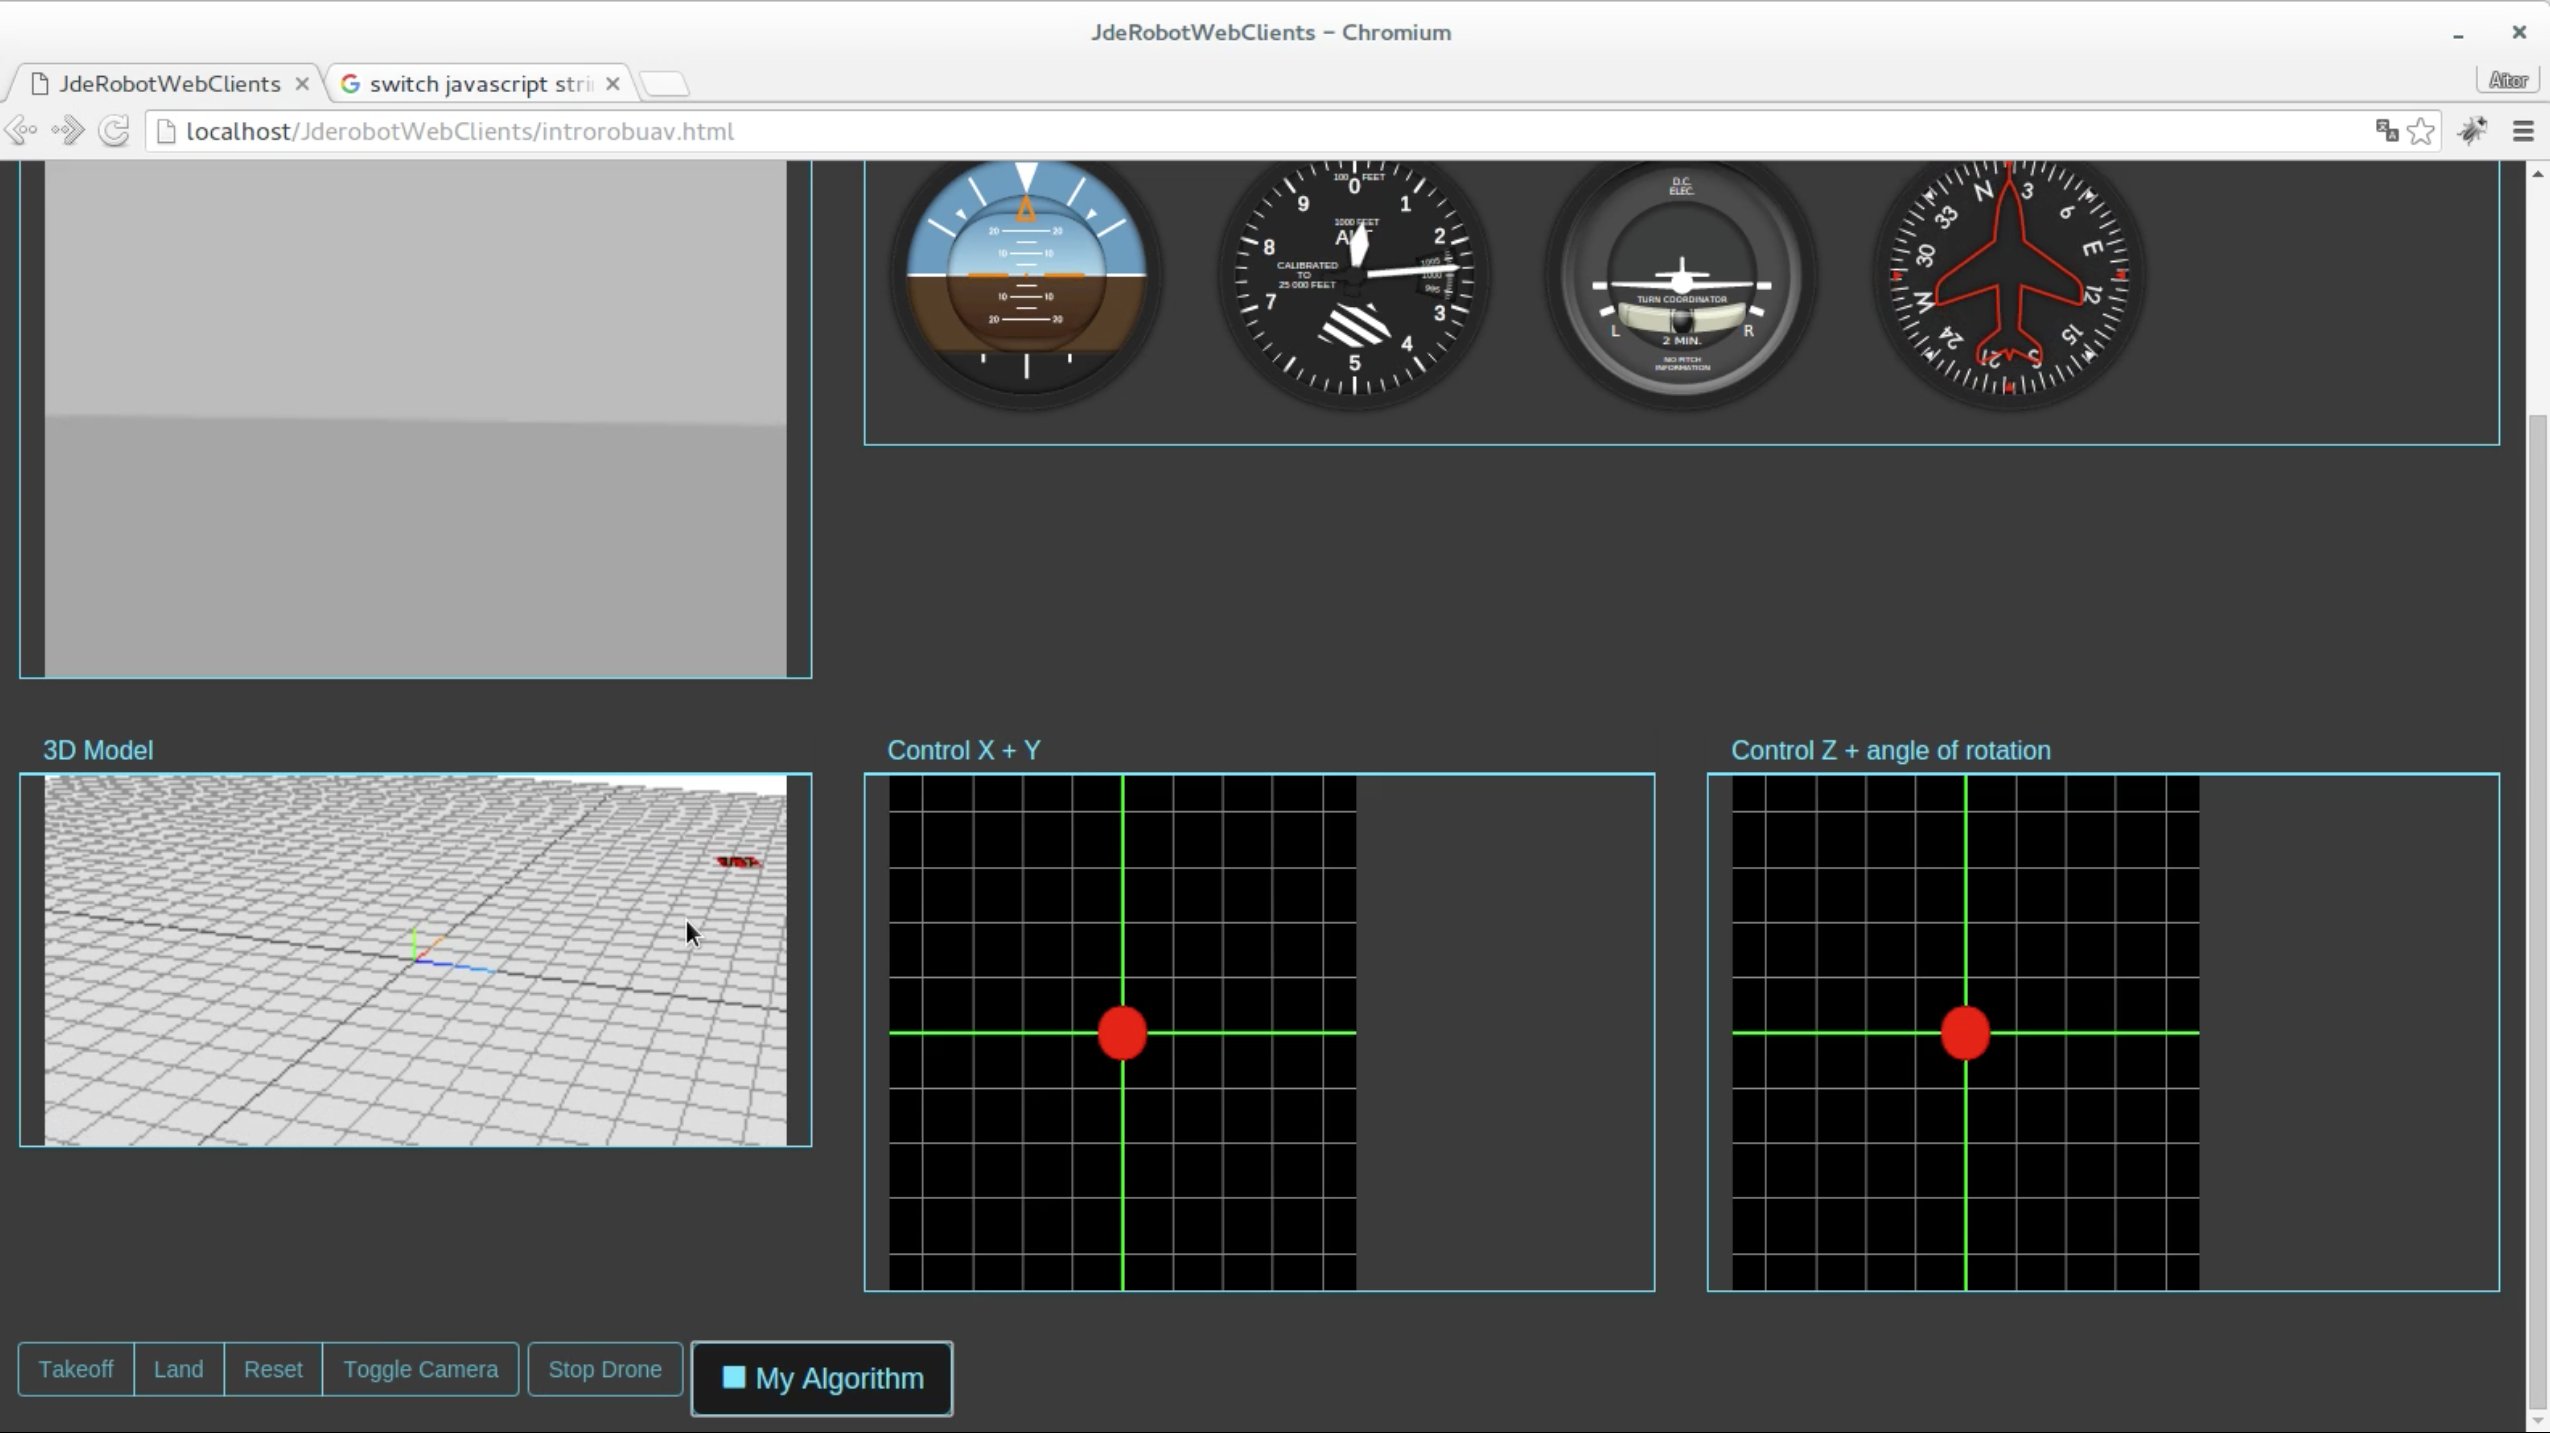
\includegraphics[width=0.9\textwidth]{introrobuavjs}
\caption{Cliente web IntrorobUavJS}
\label{fig:introrobuavjs}
\end{figure}


En el proyecto que aquí se presenta se desarrolla una aplicación web capaz de teleoperar un cuadricoptero usando los servidores desarrollados por JdeRobot para conectarnos al drone, sus sensores y actuadores, y añadiendo la tecnología web de última generación \emph{WebRTC} para establecer la conexión entre el ordenador que se comunicará con el drone y el ordenador remoto, desde el cuál se podrán ver los valores de los sensores y la cámara a bordo del drone, además como ya he mencionado, de teleoperarlo. Estas conexiones se realizarán sin el uso de servidor intermedio, usando tecnologías en tiempo real que se conectarán mediante \emph{WebSockets} de \emph{JavaScript}.\\


Una vez presentada la introducción y el contexto del proyecto en este capitulo, continuamos exponiendo los objetivos que nos hemos marcado en este proyecto. En el capítulo tres se habla sobre las infraestructuras software de las que disponemos y de las que podremos ayudarnos para el desarrollo del proyecto. Posteriormente en el capítulo cuatro veremos como hemos conseguido cumplir los objetivos marcados, exponiendo en el capítulo cinco las pruebas y experimentos que hemos realizado. En el sexto y último capitulo presentaremos las conclusiones del proyecto.\\

\chapter{Objetivos}

Una vez situado el Trabajo Fin de Grado en su contexto vamos a presentar los objetivos concretos que nos marcamos para la realización del mismo.


\section{Objetivos}

Como objetivo global nos proponemos teleoperar un drone desde dispositivos móviles cómo teléfonos o tabletas utilizando tecnologías web de ultima generación. Este objetivo se ha desglosado en tres subobjetivos concretos que explicamos a continuación.\\

Como escenario nos encontramos con un ordenador que irá a bordo del drone, y un navegador en una máquina remota. Durante toda la memoria nos referiremos como ordenador local, par local o navegador local al dispositivo que usaremos para conectarnos al cuadricóptero y el cuál deberá ir a bordo del drone, y ordenador remoto, par remoto o navegador remoto al ordenador desde el cuál teleoperaremos el vehículo.\\

\begin{itemize}


\item \emph{\textbf{Conexión local}}: Como primer subobjetivo tenemos que desarrollar una conexión directa del navegador local con el \emph{hardware} del drone. Esta conexión tiene que ser bidireccional, ya que tenemos que acceder a los sensores y actuadores del drone, así como a su cámara, pero también es necesario mandarle órdenes de movimiento.\\

Como requisito fundamental para esta conexión con el servidor de los actuadores y sensores a bordo es que tiene que ser en tiempo real y que sea lo suficientemente fluida y ligera como para que no introduzca ningún tipo de retardo.\\


\item \emph{\textbf{Conexión multimedia entre navegadores}}: El segundo punto con el que nos enfrentamos es utilizar una tecnología web moderna y actual con la que poder teleoperar el drone. Esta tecnología tiene que ser lo suficientemente versátil como para poder implementarla en nuestro proyecto. Por otro lado, al igual que la conexión local, tiene que ser bidireccional, poder transportar audio, vídeo y datos genéricos e introducir el mínimo retraso en la comunicación posible para tener una experiencia positiva y controlada del vuelo del drone.\\

Esta conexión deberá realizarse entre el ordenador local y un segundo ordenador, que será desde el que el usuario podrá teleoperar el vehículo.\\


\item \emph{\textbf{Interfaz de usuario amigable}}: Uno de los subobjetivos es desarrollar una interfaz web de usuario clara, que nos muestre de una manera lo más realista, clara y concisa posible los datos recogidos de los sensores del drone y la cámara para permitirnos conocer el estado de vuelo del drone en cada momento: altitud, inclinación, velocidad...\\

Esta interfaz deberá permitirnos el manejo del cuadricóptero de la forma mas realista y similar posible a los sistemas de control de drones que hemos hablado en la sección \ref{cap:controldrones}. Para que la experiencia de vuelo sea satisfactoria la interfaz tiene que tener unos controles de movimiento que sean sencillos, simples e intuitivos.\\

\end{itemize}


\section{Metodología y plan de trabajo}

La realización de un proyecto requiere una metodología que establezca las pautas a seguir y la planificación de las tareas que se deben llevar a cabo para cumplir los objetivos. Hemos escogido el modelo de \emph{desarrollo en espiral}, ya que es un modelo ampliamente usado en la ingeniería de \emph{software}. Este modelo define una serie de ciclos que se repiten en un bucle hasta el final del proyecto, dividiéndolo en varias subtareas más sencillas y estableciendo puntos de control al final de cada iteración en los que se evalúa el trabajo realizado y se enfocan las nuevas tareas para continuar.\\

Esta metodología recibe su nombre por la forma de espiral que tiene su representación gráfica o diagrama de flujo, que podemos ver en la figura \ref{fig:planificacion_espiral}. En cada iteración se llevan a cabo las siguientes actividades:

\begin{itemize}
 \item \textbf{Determinar los objetivos}, dividir en subobjetivos y fijar requisitos.
 \item \textbf{Analizar los riesgos} y factores que impidan o dificulten el trabajo y las consecuencias negativas que este
 pueda ocasionar.
 \item \textbf{Desarrollar} las tareas para lograr los objetivos según los requisitos especificados.
 \item \textbf{Planificar} las próximas fases tras evaluar el transcurso del proyecto.
\end{itemize}

\begin{figure}[h!]
\centering
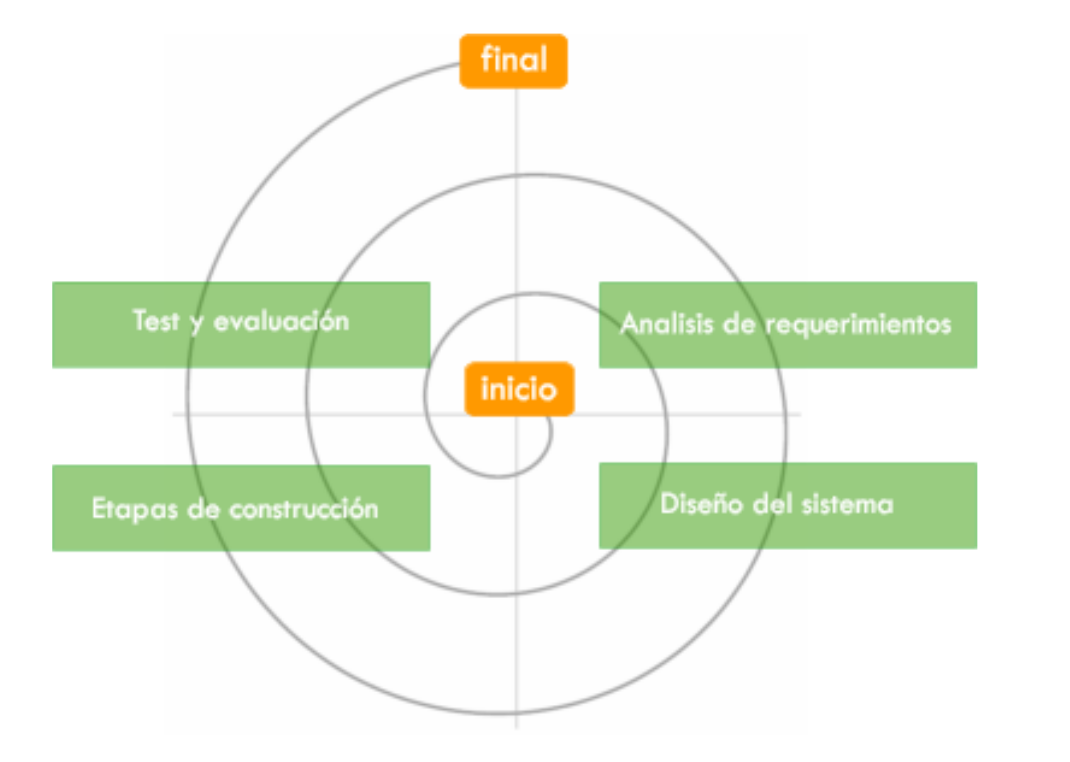
\includegraphics[width=0.9\textwidth]{espiral}
\caption{Esquema general del desarrollo del proyecto.}
\label{fig:planificacion_espiral}
\end{figure}

Durante el ciclo de vida del proyecto se han hecho reuniones periódicas con el tutor. En ellas se evaluaban los avances logrados y se marcaba la hoja de ruta a tomar para los siguientes días de desarrollo. Si los puntos marcados en sesiones anteriores no se habían finalizado se ampliaba el plazo o se intentaba buscar otra manera de avance.\\

Para facilitar el seguimiento del proyecto se ha utilizado de un mediawiki\footnote{http://jderobot.org/Irodmar-tfg} de JdeRobot en el que se iba actualizando cada avance que se lograba, con explicaciones y vídeos e imágenes. Para el código fuente se ha empleado un repositorio en la plataforma web de control de versiones GitHub\footnote{https://github.com/RoboticsURJC-students/2015-tfg-irodmar}.\\

El plan de trabajo para todo el proyecto se puede dividir en las siguientes etapas:

\begin{itemize}
\item \textbf{Familiarización con JdeRobot}: Primer contacto con esta plataforma y sus herramientas para conocer su funcionamiento.
\item \textbf{Aprendizaje de tecnologías web necesarias:} Conocer las tecnologías web que van a ser necesarias para el desarrollo del proyecto. Entre ellas se encuentra WebRTC, HTML5, CSS3, WebGL, ThreeJS, o jQuery. Primer contacto también con el \emph{middleware} ICE.
\item \textbf{Desarrollo de la conexión local:} Creación de toda la infraestructura necesaria para la interconexión entre el navegador local y el drone.
\item \textbf{Desarrollo conexión entre navegadores}: Desarrollo de la conexión remota que interconectará los dos pares.
\item \textbf{Desarrollo interfaz web de usuario}: Desarrollo de la interfaz amigable para teleoperar el drone.
\item \textbf{Experimentos}: Primero se realizan pruebas con el simulador, y cuando el código este suficientemente maduro se prueba con un drone real.
\end{itemize}







\chapter{Infraestructura Software} 

Una vez presentados los objetivos que tenemos marcados hay que echar una mirada a las tecnologías software que tenemos disponibles para utilizarlas como base y pilares del proyecto. La más importante y sobre la que está centrado el proyecto es WebRTC. Luego utilizaremos, como apoyo para cubrir las partes que WebRTC no llega, ICEJS junto con la infraestructura que tiene ya desarrollada JdeRobot.


\section{WebRTC}

WebRTC es un proyecto opensource y gratuito que nos permite tener en el navegador tecnología en tiempo real ('Real-Time Communication' ó RTC), sin plugins, a través de una simple API de JavaScript. Facilita las llamadas de voz, videollamadas, chat y compartimiento de archivos y datos. WebRTC es una tecnología Peer-to-Peer, por lo que nos permite desarrollar estas aplicaciones para que funcionen directamente desde un navegador a otro sin pasar por servidor intermedio. \\

En todo el documento nos referimos a una llamada WebRTC entre dos navegadores, pero hay que tener en cuenta que en muchas ocasiones la conexión puede ser entre un navegador y algún tipo de servidor ó MCU configurado y trabajando con la API de WebRTC para ofrecernos cualquier servicio en tiempo real.\\

La API de WebRTC nos proporciona todo el set completo de funciones para manejar y crear nuestras aplicaciones, como el control y administración de la conexión, codificación/decodificación del audio/vídeo, negociación entre navegadores, control de la conexión, firewall y NAT traversal.\\

Que WebRTC no necesita un servidor no es del todo cierto, ya que sí que necesita de lo que llamamos Servidor de Señalización. Este es el encargado de establecer el primer contacto entre ellos, facilitando el intercambio de paquetes de la negociación WebRTC.\\

WebRTC está compuesto de 3 API's:

\begin{itemize}
\item getUserMedia
\item RTCPeerConnection
\item RTCDataChannel
\end{itemize}

A continuación vamos a desgranar y explicar como funciona el intercambio de paquetes de señalización así como cada una de las API's que componen WebRTC.

\subsection{Señalización} 

Señalización es el proceso de intercambio de datos y metadatos necesarios para coordinar una llamada entre navegadores con WebRTC. Para realizar esta labor WebRTC necesita de la ayuda de un servidor externo ya que la norma deja el campo de la señalización a la capa de la aplicación.\\

Entre las labores de la señalización se encuentran la detección de los peers, el intercambio de paquetes de control de la sesión como los \textit{ICE candidates} y los \textit{SDP (Session Description Protocol)}, las prestaciones que puede darnos cada peer así como cualquier otro dato o paquete necesario para realizar este 'apretón de manos' inicial.\\

WebRTC no especifica que tipo de servidor hemos de usar para estas funciones. Esto es debido a que diferentes aplicaciones pueden preferir diferentes servidores básicos o personalizados según sus necesidades. La única restricción es el uso de la arquitectura JSEP, la cuál especifica cómo debe ser la secuencia de señalización para tener una llamada exitosa.

\subsubsection{Arquitectura \textit{JSEP (JavaScript Session Establishment Protocol)}}

El servidor debe usar la arquitectura JSEP. Esta arquitectura elimina al navegador de casi todo el flujo de señalización, el cual se maneja desde JavaScript haciendo uso de dos interfaces: transfiriendo los SDP local/remoto e interactuando con la maquina de estados ICE. Esta arquitectura nos evita, entre otras cosas, que el navegador tenga que guardar estados de sesión, de tal manera que se pueden guardar en el servidor y evitar problemas si la página se recarga, por ejemplo. \\

Como ya hemos comentado, JSEP no establece un modelo particular de señalización más allá de usar uno capaz de realizar el intercambio de los SDP y ICE según la norma RFC3264 de oferta/respuesta, de tal manera que ambas partes de la llamada sepan como actuar en cada momento. JSEP nos da los mecanismos necesarios para crear estas ofertas, así como aplicarlas a las sesión.\\

El orden en que se llaman a estas mecanismos o funciones de la API es importante, por lo que la aplicación deberá saber el orden en el que tiene que llamar a cada una, convertir las ofertas en mensajes que entienda el protocolo de señalización elegido y hacer la conversión inversa con los mensajes que se reciben para obtener ofertas que entiendan as API's.\\

El manejo de las \textit{session descriptions} es simple y sencillo. Siempre que el intercambio de una oferta/respuesta es necesario, el peer que establece la llamada ó \textit{caller} crea la oferta llamando a la función \emph{createOffer()} de la API. Esta oferta puede ser modificada por la aplicación si así fuese necesario y se establece como configuración local en ese peer con \emph{setLocalDescription()} y se envía al peer remoto a través del servidor de señalización utilizado. Al recibir esta oferta el peer \textit{called} lo utiliza como configuración del otro peer con \emph{setRemoteDescription()} y utiliza \emph{createAnswer()} para crear una respuesta apropiada, la cual establece como configuración local (\emph{setLocalDescription()}) y envía la respuesta de vuelta a través del servidor de señalización. El caller al recibir la respuesta llama también a \emph{setRemoteDescription()}, y de esta manera ambos lados tienen la información del media propia y la del peer remoto.\\


\subsubsection{Descriptores de Sesión y Máquina de Estados}

Para establecer un intercambio de media, el \textit{user agent} del navegador necesita parámetros específicos para indicar al peer remoto qué es lo que va a transmitir, de la misma manera que necesita saber el media que va a recibir para saber como decodificarlo y manejarlo. Estos datos se determinan en la descripción de sesión (SDP), los cuales se intercambian en ofertas/respuestas usando las API's JSEP como ya hemos visto anteriormente.\\

Si el SDP pertenece a la parte local o remota tiene su importancia. Una vez realizado el intercambio, cada parte mirará la lista de codecs soportados por él mismo y por la otra parte, y el cruce de los resultados determinará que codecs debe enviar y cuál espera recibir. Como podemos intuir, los parámetros exactos de la transmisión solo se pueden saber una vez la oferta y la respuesta han sido intercambiados. Sin embargo, hay ocasiones en las que el caller o el que hace la oferta puede recibir media después de enviar esta pero antes de recibir la respuesta de la otra parte. Para procesar este media de manera adecuada, el manejador de caller debe conoce los detalles de la oferta antes de que la respuesta llegue.\\

Por lo tanto, para manejar los session description de manera correcta, los user agent necesitan:

\begin{itemize}
\item Conocer si el session description pertenece a la parte local o remota.
\item Conocer si el session description es una oferta o una respuesta.
\item Permitir a la oferta ser especificada independientemente de la respuesta.
\end{itemize}

Para satisfacer estas premisas JSEP aborda esto añadiendo los métodos setLocalDescription() y setRemoteDescription() y teniendo un campo en los session description indicando el tipo de sesión que se suministra.\\

JSEP también permite el uso de respuestas provisionales. Estas respuestas permiten al peer remoto o called comunicar e informar de los parámetros iniciales de la sesión al caller, de tal manera que la sesión puede comenzar mientras se espera una respuesta final posteriormente. Este concepto es importante en el modelo oferta/respuesta, ya que al recibir una de estas respuestas el caller puede liberar y usar más recursos como extra \textit{ICE candidates, TURN candidates} o vídeo decodecs. Estas respuestas provisionales no provocan ningún tipo de des-asignación o problema, por lo que pueden ser recibidas a lo largo de la llamada para estabilizar o mejorar la misma según varíen las condiciones del ancho de banda de uno de los peers, por ejemplo.\\



DIAGRAMAS CON LA MAQUINA DE ESTADOS (pagina rtcweb-wg.github.io)
LISTA DE CODECS PERMITIDOS



http://www.html5rocks.com/en/tutorials/webrtc/infrastructure/
https://www.webrtc-experiment.com/docs/WebRTC-Signaling-Concepts.html

\subsubsection{Formato de los Descriptores de Sesión}

En la especificación WebRTC, los descriptores de sesión o session descriptions están formados por mensajes \textit{SDP (Session Description Protocol)}. Este formato no es el más óptimo para manipular con JavaScript, pero es el más popular y aceptado en el campo de las comunicaciones audiovisuales en tiempo real. Este formato es el que usa JSEP para formar e intercambiar los descriptores de sesión.\\

Para facilitar el procesado en JavaScript y una futura flexibilidad, los SDP nos los genera la API como un objeto o \textit{blob}. Si en un futuro WebRTC soporta algún formato nuevo para los descriptores de sesión, estos serán fácilmente añadidos y habilitados para poder usarlos en nuestras aplicación en vez de SDP.\\


\subsubsection{Interactive Connectivity Establishment (ICE)}

Al igual que los peer tienen que intercambiar información sobre el media, también necesitan hacerlo sobre la información de \textit{network} para que los peer sean visibles entre ellos y puedan alcanzarse. ICE es una técnica usada en aplicaciones de voz, vídeo, peer-2-peer, entre otros que nos permite solucionar problemas de alcance de red entre dos ordenadores. Estos problemas son debidos a que los ordenadores suelen estar dentro de una red privada y/o firewall. Esta técnica nos permite descubrir suficiente información sobre la topología de los otros peer para encontrar una o varias rutas potenciales entre ellos.\\

Esta información ha de obtenerse de manera local en cada peer con el \textit{ICE Agent} asociado a cada objeto RTCPeerConnection. El ICE Agent es responsable de: 

\begin{itemize}
\item Reunir tuplas candidatas de IP:Puerto.
\item Realizar pruebas de conectividad entre los peers.
\item Enviar \textit{keepalives}.
\end{itemize}

Una vez se ha finalizado y configurado el proceso de session description, el ICE Agent local comienza automáticamente el proceso de descubrir todos los posibles candidatos en el peer local. Cada candidato posible se le llama \textit{ICE Candidate}:

\begin{enumerate}
\item El ICE Agent pide al sistema operativo las direcciones IP locales.
\item Consulta a un servidor \emph{STUN (Session Traversal Utilities for NAT}) externo la tupla de dirección IP pública y puerto del peer.
\item Consulta a un servidor \emph{TURN (Traversal Using Relays around NAT)} como último recurso. 
\end{enumerate}

Como podemos ver, ICE necesita de servidores externos para obtener la tupla de dirección IP y puerto públicos necesarios para el otro peer si esta fuera de la misma red local. STUN  es un protocolo estandarizado para descubrir direcciones IP publicas de equipos que están detrás de un NAT. TURN es un servidor para transmitir mensajes entre dos clientes. Este servidor solo se usará si falla la conexión Peer-2-Peer después de probar con las direcciones IP locales y las públicas obtenidas en el servidor STUN. No es obligatorio configurar estos servidores. Si la conexión entre los peer es en la misma red no necesitamos configurar servidores STUN/TURN ya que con las direcciones locales es suficiente.\\

DIAGRAMA DE ESTADOS DE ICE (PAGINA 132 (118) DEL LIBRO DE WEBRTC)

Como podemos ver en la figura, cada vez que el navegador recolecta un nuevo ICE Candidate, la función \textit{handleIceCandidate(}) se activa y es la encargada de enviar el candidato al peer remoto a través del servidor.\\
 
Cuando un ICE Candidate llega al peer remoto, se añade en RTCPeerConnection la información de sesión que ontiene ese paquete con \textit{setRemoteDescription()}, de tal manera que el ICE Agent puede empezar a hacer pruebas de conectividad para ver si puede alcanzar al otro peer.\\

Una vez los dos ICE Agent tienen una lista completa de los ICE Candidates de ambos peers, cada agente comprueba pareando ambas lista cuales funcionan. Para ello tienen una planificación de prioridades: primero direcciones IP locales, luego IP públicas y finalmente si ambas fallan servidor TURN. Cada comprobación es una peticion/respuesta STUN que el cliente realiza con un particular candidato enviando una petición STUN desde el candidato local al candidato remoto.\\

Si uno de los pares de candidatos funciona, entonces tenemos una ruta de conexión entre ambos peer. Si todos los candidatos fallan ambas conexiones RTCPeerConnection se marca como fallida o la conexión se hace a través de un servidor TURN.\\

Cuando una conexión se ha establecido correctamente cada ICE Agent continua haciendo peticiones STUN periódicas al otro peer, lo cual sirve también como \textit{keepalives}.\\

\subsection{API's}

\subsubsection{getUserMedia} 

getUserMedia es la API encargada de darnos el streaming de audio y/o vídeo. Pide permiso al usuario para acceder y utilizar los dispositivos hardware como la cámara y el micrófono. Por el momento solo esta disponible para captar el hardware de audio y vídeo anteriormente mencionado, pero se pretende mejorar y ampliar la API para que en un futuro se pueda hacer streaming de casi cualquier fuente de datos, como un disco o sensores conectados al ordenador.\\

Al llamarla nos devuelve un objeto que contiene las pistas de audio y/o vídeo. Para llamar a esta función necesitamos suministrarle las \textit{constraints} o restricciones. En esta variable le indicamos si queremos audio, vídeo, o ambas, así como las propiedades que tienen que tener estos: resolución mínima, máxima o ideal del vídeo, framerate o cámara a usar en un dispositivo móvil (frontal/trasera) son algunas de las restricciones que podemos configurar según nuestras necesidades.\\

La llamada a la función nos devuelve un \textit{callback}. Si hay éxito al llamar la función nos devuelve el objeto anteriormente mencionado y pasa a ejecutar la función callback de éxito. En caso contrario nos devuelve el código del error y llama a la función callback de fallo. Esta forma de llamar a la función desaparecerá en próximas revisiones ya que se está implementando una llamada por \textit{promises}.\\


\subsubsection{RTCPeerConnection}

Esta API es la encargada de crear la conexión Peer-2-Peer entre el navegador local y el remoto. Trabaja de manera diferente si es el que hace la llamada ( \textit{caller}) y el que recibe la llamada (\textit{called}). El proceso de conexión es comenzado por el caller, el cuál envía una oferta a peer remoto, el cuál contesta si acepta o rechaza la llamada.

\subsubsection{RTCDataChannel}


\section{ICE y ICEJS}

df

\section{JdeRobot}

dfdfdf

\section{ArDrone de Parrot}


\chapter{Solución}

Una vez nos hemos situado en el contexto en el que se ubica este proyecto, y hemos expuesto los requisitos a cumplir y las herramientas necesarias para llegar a las metas planteadas, nos adentramos a explicar en este capitulo las soluciones utilizadas para llegar a buen puerto.\\

\section{Estructura general}

Como primer problema se presentó decidir cuál de los dos ordenadores que necesitamos para la conexión WebRTC seria el que realizaría la llamada y en que momento del flujo. Este no es un problema trivial, ya que la selección de uno u otro haría que el desarrollo de la aplicación fuese completamente distinto.\\

Se optó por que el par que llevase la batuta de la conexión fuese el ordenador local, ya que este a su vez también es el encargado de  establecer la conexión con el drone. De esta manera tenemos un par que es el que actuará de maestro, estableciendo ambas conexiones en los momentos oportunos.\\

Como ya se comento en la sección \ref{sec:senalizacion} el momento en el que se envía y se recibe cada paquete de información es critico en este sistema de señalización de oferta/respuesta, por lo que el flujo de la comunicación se diseñó y se ha desarrollado como se muestra en la figura \ref{fig:flujodellamada}.\\


\begin{figure}[htb]
\centering
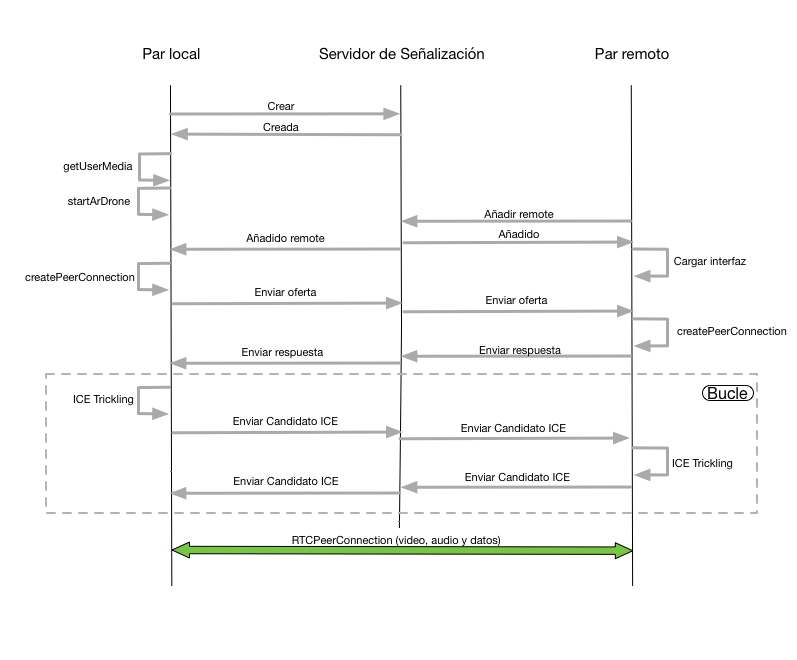
\includegraphics[width=1.1\textwidth]{diagrama_general}
\caption{Flujo de llamada del proyecto}
\label{fig:flujodellamada}
\end{figure}

Como se puede observar el par local es el que lleva la batuta de la conexión. En primer término inicia la comunicación con el servidor de señalización. Una vez que este le contesta afirmativamente a su mensaje de creación de la comunicación inicia un proceso en el que se conecta al cuadricóptero y accede a la cámara. Una vez realizados estos dos procesos espera a que un par remoto quiera unirse a la conexión.\\

Cuando el par remoto accede a servidor de señalización, este le envia un mensaje al par local indicando que un par remoto se ha conectado. En este momento el par local inicia la creación de la conexión \emph{RTCPeerConection} de WebRTC. Primero se produce el intercambio de paquetes SDP a través del servidor de señalización, y posteriormente el de ICE. Una vez finalizados ambos ya tenemos establecida la conexión WebRTC entre ambos pares.\\

\section{Conexión con la API del drone}

Esta primera parte la hemos solucionado dividiendo el problema en dos subproblemas. Por un lado la conexión con el servidor encargado de conectarse al cuadricóptero, \emph{ardone\_server}, y por otro obtener un flujo de vídeo para poder visualizarlo en la parte remota. Este problema lo hemos solucionado incorporando una cámara a bordo del drone que ira conectada al par local y a la cual accederemos desde el navegador con la API getUserMedia que nos brinda WebRTC.\\

Se explica a continuación la conexión con el servidor y posteriormente el acceso a la cámara con getUserMedia.\\


\subsection{ArDrone\_server, ICE y WebSockets}

Para establecer la conexión con el drone se ha utilizado el componente \texttt{ardrone\_server} de JdeRobot. Este componente tiene dos versiones, la componente simulada que es la que hemos instalado en forma de plugin en el simulador Gazebo y la componente real, que se conecta al drone real. Ambas componentes nos ofrecen las mismas interfaces de conexión, por lo que una única configuración de nuestra aplicación bastará para poder trabajar con la versión simulada y la real.\\

En este punto podemos dividir el proyecto en dos partes. Servidor y Cliente. La parte de servidor trataremos básicamente la configuración, y la parte del cliente será la que se desarrolla desde cero.\\

\subsubsection{Servidor}

Los componentes JdeRobot utilizan, como ya hemos visto, interfaces ICE para el intercambio de información del que se ocupan. Los navegadores no tienen capacidad de usar el \emph{middlewre} ICE directamente. Para poder conectarnos con estas interfaces ICE hemos tenido que instalar el plugin ICE for JavaScript, o ICE\-JS. Este plugin nos habilita la opción de conectarnos a estas interfaces directamente desde el navegador usando \emph{websockets}.\\

Aunque estaba disponible la versión 3.6 de ICE\footnote{https://doc.zeroc.com/display/Ice36/Home} la cuál trae en la suite instalado de serie ICE\_JS, hemos usado la versión 3.5, ya que es la versión compatible con la versión más actual de JdeRobot\footnote{http://jderobot.org/Manual-5}. En esta versión ICE\_JS es un plugin a parte el cuál hay que instalarlo descargando el código fuente desde la página de Zeroc\footnote{https://zeroc.com} y compilarlo.\\

Una vez instalado hay que activar este plugin en el servidor. Para ello hay que añadir la siguiente línea en el archivo de configuración del servidor:\\

\begin{lstlisting}[caption=Activación del plugin ICEJS]
# ICE-JS
Ice.Plugin.IceWS=IceWS:createIceWS
\end{lstlisting}

Posteriormente a esto, en el mismo archivo hay que indicarle las direcciones IP y los puertos de cada interfaz de conexión. Cada conexión se corresponderá con un \emph{WebSocket}, y la nomenclatura es la siguiente:\\

\begin{lstlisting}[caption=Formato \emph{endpoints} de los \emph{WebSocket} de ICEJS]
# ICE-JS
:ws -h ip -p puerto
\end{lstlisting}


El servidor tiene hasta un máximo de seis interfaces diferentes a las que te puedes conectar. Cada uno de estas interfaces nos ofrece un servicio diferente. Para nuestro proyecto hemos usado cuatro de esas interfaces.

\begin{itemize}
\item \textbf{Pose3D:} Con esta interfaz accedemos a los datos \emph{pose} del cuadricóptero (x, y, z, h y \emph{quaternion}).
\item \textbf{Navdata:} Esta interfaz nos proporciona los datos de navegación procedentes de los sensores, como la velocidad de las componentes (x, y, z) del drone, altitud, la velocidad del viento, el nivel de batería, etc.
\item \textbf{CMDVel:} Esta interfaz es la que se encarga de recibir las órdenes de movimiento.
\item \textbf{BaseExtra:} Esta interfaz nos da funcionalidades extra como el aterrizaje o el despegue del cuadricóptero.
\end{itemize}

Así pues, esta es la forma final que tiene nuestro archivo de configuración:\\

\begin{lstlisting}[caption=Archivo de configuración]
# Ice-JS
Ice.Plugin.IceWS=IceWS:createIceWS

# Variables de control para ver traceroutes de las conexiones ICE.
#Ice.Trace.Network = 3
#Ice.Trace.Protocol=1


ArDrone.Pose3D.Endpoints=default -h 0.0.0.0 -p 9998:ws -h 0.0.0.0 -p 19000
ArDrone.Pose3D.Name=ardrone_pose3d

ArDrone.RemoteConfig.Endpoints=default -h 0.0.0.0 -p 9997
ArDrone.RemoteConfig.Name=ardrone_remoteConfig

ArDrone.Navdata.Endpoints=default -h 0.0.0.0 -p 9996:ws -h 0.0.0.0 -p 15000
ArDrone.Navdata.Name=ardrone_navdata

ArDrone.CMDVel.Endpoints=default -h 0.0.0.0 -p 9995:ws -h 0.0.0.0 -p 11000
ArDrone.CMDVel.Name=ardrone_cmdvel

ArDrone.Extra.Endpoints=default -h 0.0.0.0 -p 9994:ws -h 0.0.0.0 -p 17000
ArDrone.Extra.Name=ardrone_extra

ArDrone.NavdataGPS.Endpoints=default -h 0.0.0.0 -p 9993
ArDrone.NavdataGPS.Name=ardrone_navdatagps
\end{lstlisting}

A parte de los \emph{endpoints} es también importante configurar correctamente el nombre de cada uno de las interfaces, ya que será necesario para una correcta conexión desde el navegador. La dirección ip \texttt{0.0.0.0} indica que la dirección de escucha del servidor es la ip local del equipo. \\


\subsubsection{Cliente}

Una vez configurado el servidor hemos creado el método ArDrone.js, el cuál es el encargado de conectarse y manejar la conexión con el servidor \texttt{ardrone\_server}.\\

Para establecer una comunicación ICE lo primero es crear las variables ICE necesarias. Estas las creamos de la siguiente manera:\\

\begin{lstlisting}[caption=Formato \emph{endpoints} de los \emph{WebSocket} de ICEJS]
// Variable ICE para la conexion
var id = new Ice.InitializationData();
id.properties = Ice.createProperties();
id.properties.setProperty("Ice.Trace.Network", "3"); // Propiedad para tracear la conexion
id.properties.setProperty("Ice.Trace.Protocol", "1"); // Propiedad para tracear la conexion
var communicator = Ice.initialize(id);
\end{lstlisting}

Por si fallase la comunicación ICE se le ha añadido a la variable \emph{id} una propiedad con la que podemos seguir la ruta de la comunicación y detectar en que punto se produce el fallo.\\

Posteriormente es necesario crear una variable, que será la que actuará como \emph{proxy}, por cada interfaz a la que necesitemos conectarnos. Esta es la nomenclatura que debe seguir:\\

\begin{lstlisting}[caption=Nomenclatura de variable que actuará como \emph{proxy}]
var proxy = communicator.stringToProxy("nombre_interfaz:ws -h " + ip + " -p " + "puerto");
\end{lstlisting}

Nótese en la nomenclatura donde pone \emph{nombre\_interfaz} se corresponde con el nombre que le hemos asignado al \emph{endpoint} en el archivo de configuración del servidor. Asimismo el puerto también se corresponde con el configurado.\\


La comunicación con las interfaces se realiza mediante el objeto promesa o \emph{promise}. Este objeto se usa para las comunicaciones asíncronas y se caracteriza por tener tres estados: pendiente, cumplida o rechazada. Cuando una promesa ha sido llamada puede presentar el estado cumplida o rechazada, lo que nos permite llamar al argumento correspondiente y poder actuar en consonancia. De esta manera podemos hacer que métodos asíncronos actúen como métodos sincronos.\\

El núcleo de la conexión con el servidor \emph{ardrone\_server} queda como sigue:\\

\begin{lstlisting}[caption=Nucleo ArDrone]
// base extra connection
var baseextra = communicator.stringToProxy("ardrone_extra:ws -h " + ip + " -p " + baseextraPort);
jderobot.ArDroneExtraPrx.checkedCast(baseextra).then(
    function(ar){
        extraProxy = ar;
        console.log("extraProxy connected: " + ar);
    },
    function(ex, ar){
        console.log("extraProxy NOT connected: " + ex);
    }
);               

// NavData
var basenavdata = communicator.stringToProxy("ardrone_navdata:ws -h " + ip + " -p " + navdataProxyPort);
jderobot.NavdataPrx.checkedCast(basenavdata).then(
    function(ar){
        console.log("navdataProxy connected: " + ar);
        navdataProxy = ar;
        navdataProxy.getNavdata().then(
        function(navdata){
            if (navdata.vehicle == ARDRONE_SIMULATED) {
                virtualDrone = true;
                console.log("virtualDrone = true");
            } else {
                virtualDrone = false;
                console.log("virtualDrone = false");
            }
        },
        function (ex, ar){
            console.log("Fail getNavdata() function: " + ex);
        }
        );
    },
    function (ex, ar){
        console.log("navdataProxy NOT connected: " + ex);
    }        
);        

// CMDVelPrx
var basecmdVel = communicator.stringToProxy("ardrone_cmdvel:ws -h " + ip + " -p " + cmdVelProxyPort);
jderobot.CMDVelPrx.checkedCast(basecmdVel).then(
    function(ar){
        console.log("cmdVelProxy connected: " + ar);
        cmdVelProxy = ar;
    },
    function(ex, ar){
        console.log("cmdVelProxy NOT connected: " + ex);
    }
);             

// Pose3D
var basepose3D = communicator.stringToProxy("ardrone_pose3d:ws -h " + ip + " -p " + pose3DProxyPort);
jderobot.Pose3DPrx.checkedCast(basepose3D).then(
   function(ar){
       console.log("pose3DProxy connected: " + ar);
       pose3DProxy = ar;
        window.po = pose3DProxy;
        resolve("Stuff worked!");
       pose3DProxy.getPose3DData().then(
           function (ar){
               console.log("getPoseDData().");
               pose = ar;
           },
           function(ex, ar){
               console.log("Fail call getPoseDData().");
           });
   },
   function(ex, ar){
       console.log("pose3DProxy NOT connected: " + ex)
   }
);
\end{lstlisting}

En este punto ya estamos conectados con las interfaces del servidor, y por consiguiente, con el drone. Para poder teleoperar el drone hay que crear unas funciones que serán los manejadores. Por un lado hemos creado las funciones de aterrizaje y de despegue. Estas funciones utilizan la interfaz \emph{ardrone\_extra}:\\

\begin{lstlisting}[caption=Funciones aterrizaje y despegue.º]
// extraProxy functions  
function takeoff() {
    extraProxy.takeoff().then(
        function(ar){
            console.log("Take Off.");
        },
        function(ex, ar){
            console.log("Take Off failed.")
        }
     );
}
    
function land() {
        extraProxy.land().then(
        function(ar){
            console.log("Landing.");
        },
        function(ex, ar){
            console.log("Landing failed: " + ex)
        }
     );
}
\end{lstlisting}

Las interfaces \emph{Navdata} y \emph{Pose3D} so las encargadas de suministrar todos los datos de navegación de los sensores. Las funciones con las que accedemos a estas interfaces y actualizamos todos estos datos son las siguientes:\\

\begin{lstlisting}[caption=Variables actualización datos de los sensores.]

function updateNavData() {
    navdataProxy.getNavdata().then(
        function(ar){
            navdata = ar;
            //console.log("updateNavData()");
        },
        function (ex, ar){
            console.log("Fail getNavdata() function." + ex)
        }        
    );    
}

function updatePose(){
    pose3DProxy.getPose3DData().then(
            function (ar){
                pose=ar;
                //console.log("getPose3DData. ")
            },
            function(ex, ar){
                console.log("Fail call getPoseDData(): " + ar2);
            });   
}

\end{lstlisting}


Llamando a estas funciones periódicamente tenemos actualizados los datos de navegación procedentes de los sensores: brújula, posición, velocidad, altitud...\\

Para poder teleoperar el drone se ha implementado una función que es la encargada de enviarle las órdenes de movimiento.\\

\begin{lstlisting}[caption=Función manejadora de las órdenes.]

function sendVelocities () {
    cmdVelProxy.setCMDVelData(cmd).then(
        function(ar){
          //console.log("sendVelocities.");
        },
        function(ex, ar){
          console.log("sendVelocities failed.")
        }
    );
}

\end{lstlisting}

Dónde la variable \emph{cmd} contiene los parámetros que necesita el drone para moverse. Esta variable es una variable CMDVel de JdeRobot y tiene esta estructura:\\

\begin{lstlisting}[caption=Variable CMD]

var cmd = new jderobot.CMDVelData; 
cmd.linearX=0.0;
cmd.linearY=0.0;
cmd.linearZ=0.0;
cmd.angularZ=0.0;
cmd.angularX=0.0;
cmd.angularY=0.0;

\end{lstlisting}




\subsection{getUserMedia}

La interfaz que no hemos implementado de las que nos ofrece el servidor \texttt{ardrone\_server} es la interfaz \emph{cameraserver}. Esta interfaz se encarga de recoger las imágenes de la cámara integrada en el drone. Para tener una imagen con mas resolución y que nos permita visualizar con mayor calidad se ha optado por colocar una cámara a bordo y acceder a ella con las herramientas que nos suministra WebRTC.\\

Esta camara se conecta a nuestro ordenador local a través de una conexión USB. Camara y MiniPC vana a bordo del drone. Como WebRTC aún no es una norma, para acceder a la cámara desde cualquier navegador debemos crear una variable que sea compatible con todos los que tengan implementado las APIs de WebRTC. Para ello hay que añadirle los prefijos correspondientes de cada navegador:\\


\begin{lstlisting}[caption=Variable de getUserMedia.]
navigator.getUserMedia = navigator.getUserMedia || navigator.webkitGetUserMedia || navigator.mozGetUserMedia;
\end{lstlisting}


Acceder a la cámara a con \emph{GetUserMedia} se hace a través de una función que admite dos llamadas de vuelta o \emph{callback}. Uno de ellos es el callback de éxito, y el segundo el de error. Según sea de exitosa el acceso a la cámara se llamara a una función u otra. Si nos devuelve éxito se llama a una función con la que guardaremos el streaming y lo visualizaremos en un elemento vídeo de HTML5, si devuelve error mostramos un mensaje del error ocurrido.\\

\begin{lstlisting}[caption=getUserMedia.]

// Manejador de exito
function handleUserMedia(stream){
	localStream = stream;

	if (window.URL){
		localVideo.src = window.URL.createObjectURL(stream);
	} else{
		localVideo.src = stream;
	}
	//console.log('Adding local stream.');
	// Envio un mensaje al servidor como ack de exito al llamar gerUserMedia()	
}

// manejador de error
function handleUserMediaError(error){
	console.log('getUserMedia error: ', error);
}

//Funcion getUserMedia
navigator.getUserMedia(constraints, handleUserMedia, handleUserMediaError); 

\end{lstlisting}

El primer argumento de la función es una variable en la que le indicamos las restricciones que queremos: audio, vídeo, solo uno de ellos, resoluciones... Las restricciones elegidas para nuestro proyecto son las siguientes:\\

\begin{lstlisting}[caption=Restricciones de getUserMedia]

var constraints = {
    audio: false,
    video: {
        width: { ideal: 1280, max: 1920 },
        height: {ideal: 720, max: 1080 },
    }
};

\end{lstlisting}

Sólo accedemos al vídeo de la cámara, ya que el audio no lo necesitamos para el proyecto. Por otro lado indicamos una resolución ideal, de 1280x720 píxeles. Si la cámara que le conectamos al ordenador tiene más capacidad restringimos su resolución a HD (1920x1080 píxeles).\\

El flujo que nos proporciona \emph{getUserMedia} lo utilizaremos con \emph{RTCPeerConnection} en para enviárselo al par remoto.\\

\section{Uso WebRTC para el control del drone}

Interconectar el ordenador remoto al drone a través de otro ordenador es el segundo de los objetivos marcados. Para ello vamos a utilizar WebRTC y por su comunicación entre pares. El primer paso es construir un servidor de señalizacion.\\

\subsection{Señalización}

Las necesidades a cubrir en cuanto al servidor de señalización es que sea capaz de intercambiar los datos de red necesarios (Candidatos ICE) y de paquetes SDP. El intercambio debe hacerse con el protocolo de oferta/respuesta según lo establecido en la arquitectura JSEP explicada con anterioridad.\\

Se ha optado por desarrollar el servidor escrito en el lenguaje de programación \emph{Node.js}\footnote{https://nodejs.org/}. Las razones por las que hemos elegido este servidor es que está escrito en JavaScript, por lo que nos resulta muy útil al utilizarse el mismo lenguaje de programación que vamos a utilizar para el resto del proyecto. Por otro lado es un servidor muy liviano.\\

Para cumplir con la arquitectura JSEP vamos a utilizar la librería \emph{Socket.io}\footnote{http://socket.io}, la cuál nos facilita el desarrollo de aplicaciones con necesidades de conexión entre equipos a través de \emph{Websockets}.\\

Como se puede ver en la figura \ref{fig:flujodellamada}, al servidor se le envían 4 tipos de paquetes. Cuando se conecta el par local, cuando se conecta el par remoto, intercambio de candidatos ICE e intercambio de SDP. Sabiendo que tanto los candidatos ICE como los paquetes SDP son objetos, decidimos crear el servidor aceptando tres diferentes tipos de paquetes: el inicial del par local, el inicial del par remoto, y mensajes genéricos que contendrían los objetos anteriormente mencionados. Así pues, esta es la forma del código que gestiona en el servidor el intercambio de paquetes para la señalización.\\

\begin{lstlisting}[caption=Nucleo servidor de señalización]

io.sockets.on('connection', function (socket){

	// Manejaador de mensajes genericos 'message' (intercambios SDP y Candidatos ICE)
	socket.on('message', function (message) {
		//log('Server --> got message: ', message);
		// Si el que envia es Droner hay que mandarlo al remote
		if (socket.id == dronerID) {
			io.sockets.socket(newPeer).emit('message', message);
		// Si el que envia es remote hay que mandarselo al droner
		} else if (socket.id== newPeer) {
			io.sockets.socket(dronerID).emit('message', message);
		} 
	});

	// manejador de mensjes 'create'  enviados por Droner
	socket.on('create', function () {
		//log('Server --> Droner has sido conectado');
		socket.join();
		dronerID = socket.id;
		socket.emit('created');
	});
	

	// Manejador de mensajes 'join remote ' enviados por remote
	socket.on('join remote', function () {
		//log("Server --> Un 'remote' se ha unido.");
		
		io.sockets.in().emit('join remote');
		socket.join();
		newPeer = socket.id;
		socket.emit('joined');
	});
});
\end{lstlisting}

Una vez tenemos el servidor operativo vamos a explicar como hemos creado la conexión entre pares y como hemos usado esta conexion para transmitir el vídeo de la cámara del drone hasta el par remoto.\\

\subsection{RTCPeerConnection: Transmisión de la cámara a bordo}

La conexión entre pares se crea en el momento en el que el par local recibe del servidor de señalizacion un mensaje indicando que el par remoto se ha conectado y esta preparado para crear la conexión. En ese momento se ejecuta una función que configura los parámetros necesarios y  crea la comunicación.\\

Al igual que getUserMedia debemos configurar las variables necesarias para que sean compatibles con todos los navegadores. Para establecer la conexión necesitamos tres variables distintas:\\


\begin{lstlisting}[caption=Variables WebRTC]

RTCPeerConnection = window.RTCPeerConnection || window.mozRTCPeerConnection || 
                       window.webkitRTCPeerConnection || window.msRTCPeerConnection;
RTCPSessionDescription = window.RTCSessionDescription || window.mozRTCSessionDescription ||
                       window.webkitRTCSessionDescription || window.msRTCSessionDescription;
RTCIceCandidate = window.RTCIceCandidate || window.mozRTCIceCandidate ||
                        window.webkitRTCIceCandidate || window.msRTCIceCandidate;

\end{lstlisting}

\begin{itemize}

\item \emph{RTCPeerConnection}: Esta variable es la encargada de crear y mantener la conexión entre pares. Esta variable neesitará de las otras dos para crear la conexión.
\item \emph{RTCPSessionDescription}: Crea los SDP locales y se encarga de gestionar los SDP recibidos.
\item \emph{RTCIceCandidate}: Encargada de descubrir los Candidatos ICE y de gestionar los recibidos del otro par.

\end{itemize}


También debemos indicarle los servidores STUN y TURN a los que conectarse para averiguar los pares de ip y puerto para los Candidatos ICE:\\

\begin{lstlisting}[caption=Servidores STUN y TURN]

var ICE_config = {
  'iceServers': [
    {
      'urls': 'stun:stun.l.google.com:19302'
    },
    {
      'urls': 'stun:23.21.150.121'
    },
    {
      'urls': 'turn:192.158.29.39:3478?transport=udp',
      'credential': 'JZEOEt2V3Qb0y27GRntt2u2PAYA=',
      'username': '28224511:1379330808'
    },
    {
      'urls': 'turn:192.158.29.39:3478?transport=tcp',
      'credential': 'JZEOEt2V3Qb0y27GRntt2u2PAYA=',
      'username': '28224511:1379330808'
    }
  ]
};

\end{lstlisting}

Una vez tenemos las variables configuradas, la forma en la que creamos la conexión WebRTC es la siguiente:\\

\begin{lstlisting}[caption=RTCPeerConnection.]

var PeerConnection = new RTCPeerConnection(ICE_config, pc_constraints);

\end{lstlisting}

Esta función admite dos argumentos. El primero es la configuración ice que ya hemos visto y el segundo es una variable con las restricciones de todas las funcionalidades y configuraciones que tiene RTCPeerConnection. En nuestro caso esa variable está vacía ya que la configuración por defecto es más que adecuada para nuestros intereses.\\

Para que el intercambio de paquetes en la señalización hay que crear los manejadores que RTCPeerConnection necesita para los SDP y para los Candidatos ICE. El par local tiene sus manejadores ya que es el encargado de llevar la batuta de la conexión, y en el par remoto tienen otros manejadores difentes. \\

Los SDP se manejan en el par local con el método \emph{createOffer} que al ser llamado activa el proceso de crear la oferta SDP. Cada vez que crea uno nuevo salta un evento en la función que se le ha indicado, llamada \emph{gotLocalDescription}. Esta función se encarga de ajustar el SDP local al SDP que se acaba de crear y de mandárselo al otro par a través del servidor de señalización. Si al crear un SDP se produce un error se llama a la función de error, la cual se encargara de notificárnoslo en la consola del navegador.\\


\begin{lstlisting}[caption={Manejandor de los SDP.}, label={lst:manejadorsdp}]

// Funcion de exito
function gotLocalDescription(sessionDescription){
  PeerConnection.setLocalDescription(sessionDescription, successLocalSDP, errorLocalSDP);
  sendMessage(sessionDescription);
}

// Funcion de error
function onSignalingError(error){
  console.log('Fallo al crear el SDP: ' + error);	
}

// Metodo manejador de las SDP
PeerConnection.createOffer(gotLocalDescription, onSignalingError);

\end{lstlisting}

Esta oferta es recibida en el par remoto a través del servidor de señalización y se guarda como la oferta del otro par, ya que la necesitaremos para conocer las características del flujo audiovisual que nos llegará:\\


\begin{lstlisting}[caption={Estableciendo SDP del par remoto.}]
PeerConnection.setRemoteDescription(new RTCPSessionDescription(message));
\end{lstlisting}

Al establecer el SDP remoto ocurre un evento del método \emph{createAnswer} y crea una respuesta a la oferta recibida.\\

\begin{lstlisting}[caption=Manejandor de respuestas SDP]
PeerConnection.createAnswer(gotLocalDescription, onSignalingError);
\end{lstlisting}


Las funciones de éxito y error \emph{gotLocalDescription} y \emph{onSignalingError} son las mismas que en el otro par, hemos mostrado su código en el listing \ref{lst:manejadorsdp}.\\

Para manejar los Candidatos ICE utilizamos un método manejador \emph{onicecandidate}, el cuál llama a la función indicada, \emph{handleIceCandidate()}, en el momento en que se encuentra un Candidato ICE. Esta función se encarga de enviar el candidato a través del servidor de señalización. Ambos pares usan este mismo evento con la misma configuración.\\

\begin{lstlisting}[caption=Manejandor de los Candidatos ICE locales.]

function handleIceCandidate(event){
  //console.log('handleIceCandidate event: ', event);
  if (event.candidate) {
    sendMessage({
    type: 'candidate',
    label: event.candidate.sdpMLineIndex,
    id: event.candidate.sdpMid,
    candidate: event.candidate.candidate});
  } else {
    console.log('End of candidates.');
  }
    // console.log('Local ICE candidate: \n' + event.candidate.candidate);
  
}

// Metodo manejador de candidatos ICE
PeerConnection.onicecandidate = handleIceCandidate; // Manejador ICE local (manda ICE local a remoto)

\end{lstlisting}

Los candidatos son recibidos en los pares a través del servidor de señalización. Se crea el candidato y se le añade como candidato remoto con el método \emph{addIceCandidate}.\\

\begin{lstlisting}[caption=Manejandor de los Candidatos ICE remotos.]
var candidate = new RTCIceCandidate({sdpMLineIndex:message.label,candidate:message.candidate});
PeerConnection.addIceCandidate(candidate);
\end{lstlisting}


Uno de los puntos mas importantes para el proyecto que se tiene que encargar \emph{RTCPeerConnection} es transferir el flujo visual desde el par local al par remoto. WebRTC nos lo permite de una forma muy sencilla. En el par local, con un método al que le añadimos como argumento el flujo que hemos obtenido llamar a la API \emph{getUserMedia}:\\

\begin{lstlisting}[caption=Manejandor del flujo audiovisual en el par local.]
PeerConnection.addStream(localStream); 
\end{lstlisting}

Y en el par remoto con un método manejador llamado \emph{onaddstream}, que en el momento de saltar un evento llama a la función \emph{handleRemoteStreamAdded}, y esta se encarga de configurar el flujo en una etiqueta vídeo de HTML5.\\

\begin{lstlisting}[caption=Manejandor del flujo audiovisual en el par remoto.]

// Funcion manejadora
function handleRemoteStreamAdded(event) {
	window.remoteVideo = remoteVideo; // make avalaible on console for inspection
    var remoteVideo = document.getElementById("droneVideo"); // 

	if (window.URL){
		remoteVideo.src = window.URL.createObjectURL(event.stream);
	} else{
		remoteVideo.src = event.stream;
	}
    //console.log('Remote stream attached!!.');
	remoteStream = event.stream;
}

// Metodo manejador 
PeerConnection.onaddstream = handleRemoteStreamAdded;
\end{lstlisting}

Una vez creada y establecida la conexión \emph{RTCPeerConnection} la usaremos para crear la conexión de datos \emph{RTCDataChannel}, para transportar toda la información necesaria hacia ambos lados.\\


\subsection{RTCDataChannel}
\subsubsection{Sensores de navegación}
\subsubsection{Órdenes}
\subsubsection{Localización espacial del drone}


\section{Interfaz amigable y actual}
\subsection{Visualización de las imágenes}
\subsection{Joysticks}
\subsection{Relojes de navegación}
\chapter{Experimentos}

En capítulos anteriores se han expuesto los objetivos marcados para la realización del proyecto así como la solución desarrollada para cada uno de estos problemas y las herramientas utilizadas para los mismos. En este capítulo se muestran los experimentos que se han ido realizando según íbamos cumpliendo objetivos y que sirven como validación experimental de la solución programada.\\

\section{Experimentos con simulador Gazebo}

Una vez desarrollado el proyecto y satisfaciendo todos los objetivos marcados se han realizado pruebas sobre el drone simulado en Gazebo para comprobar sin ningún tipo de riesgos el funcionamiento del mismo.\\

\begin{figure}[h!]
\centering
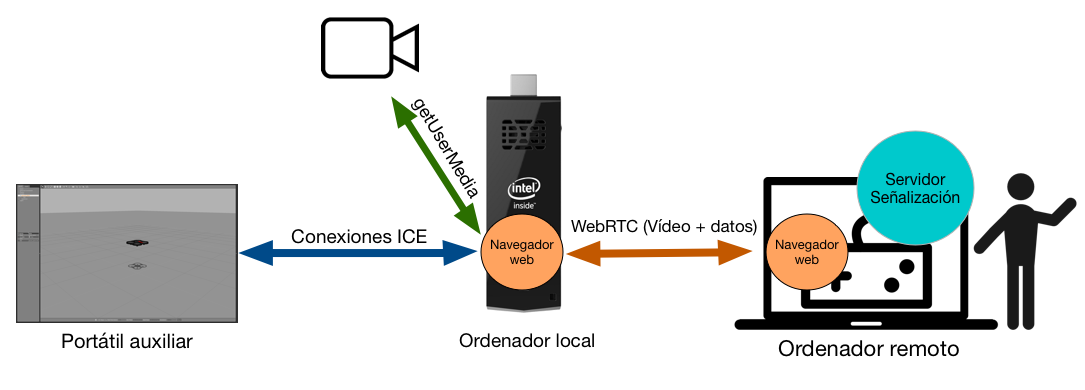
\includegraphics[width=0.9\textwidth]{experimento1}
\caption{Experimento con el simulador Gazebo y un ordenador remoto.}
\label{fig:esquemaexperimento1}
\end{figure}

Para realizar este experimento de la manera más realista al experimento final con el drone real se ha utilizado un \emph{Intel Compute Stick}\footnote{\url{http://www.intel.com/content/www/us/en/compute-stick/compute-stick-product-brief.html}} como par local. El navegador en ese \emph{computer stick} es el encargado de conectarse a las interfaces ICE que nos proporciona el plugin ArDrone desarrollado por JdeRobot para el simulador Gazebo. Este ordenador está compuesto por un procesador Intel Atom que corre Ubuntu 14.04 LTS como sistema operativo. El simulador Gazebo se ha ejecutado en un portátil auxiliar y utilizaremos otro equipo portátil como par remoto desde el que teleoperaremos el drone además de ejecutar el servidor de señalización. La figura \ref{fig:esquemaexperimento1} muestra el esquema del montaje de este experimento. \\

Los resultados de este experimento han sido muy positivos, el control y manejo del drone han sido de manera fluida y sin realizar ningún movimiento extraño producido por algún tipo de mal funcionamiento del código. El manejo se ha realizado tanto con los \emph{joysticks} virtuales como con el mando. Se puede ver un fotograma del vídeo\footnote{\url{http://jderobot.org/Irodmar-tfg#WebRTC_on_a_drone_working_with_Gazebo5}} del experimento en la figura \ref{fig:experimentogazebo}.\\

\begin{figure}[h!]
\centering
\includegraphics[width=0.9\textwidth]{experimentogazebo}
\caption{Experimento con el simulador Gazebo.}
\label{fig:experimentogazebo}
\end{figure}

En la siguiente figura (\ref{fig:secexp1}) se puede observar la secuencia de movimiento del drone durante el experimento.\\

\newpage
\begin{figure}[h!]
\centering
  \begin{subfigure}[]{47mm}
    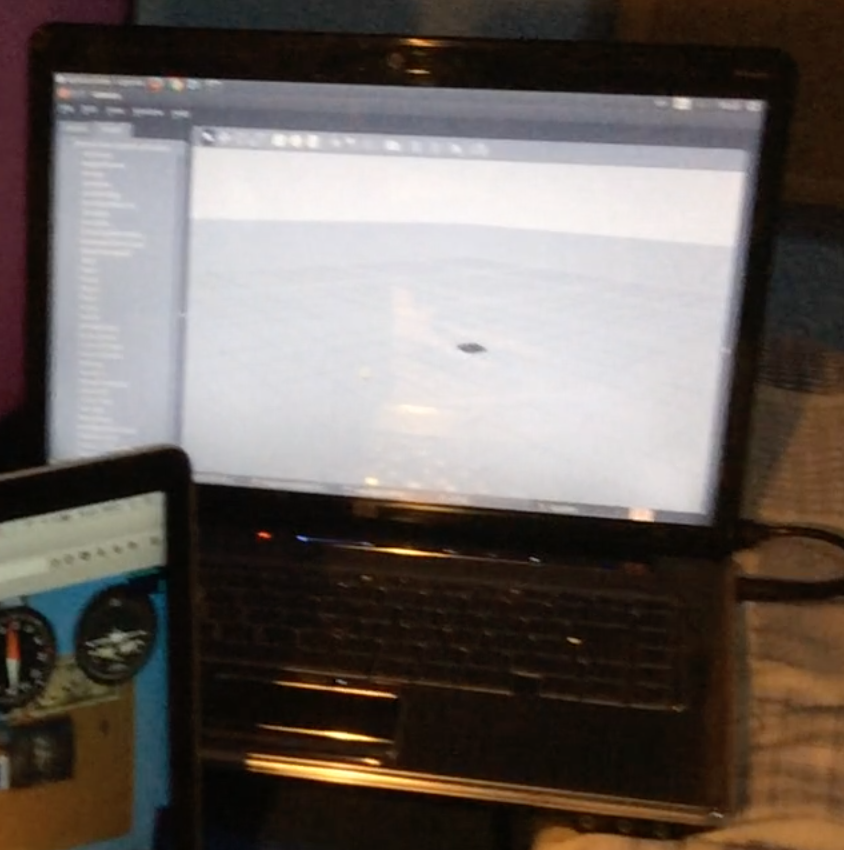
\includegraphics[width=47mm]{sec_exp1_1}
  \end{subfigure}
  \hspace{0.5pt}
  \begin{subfigure}[]{47mm}
    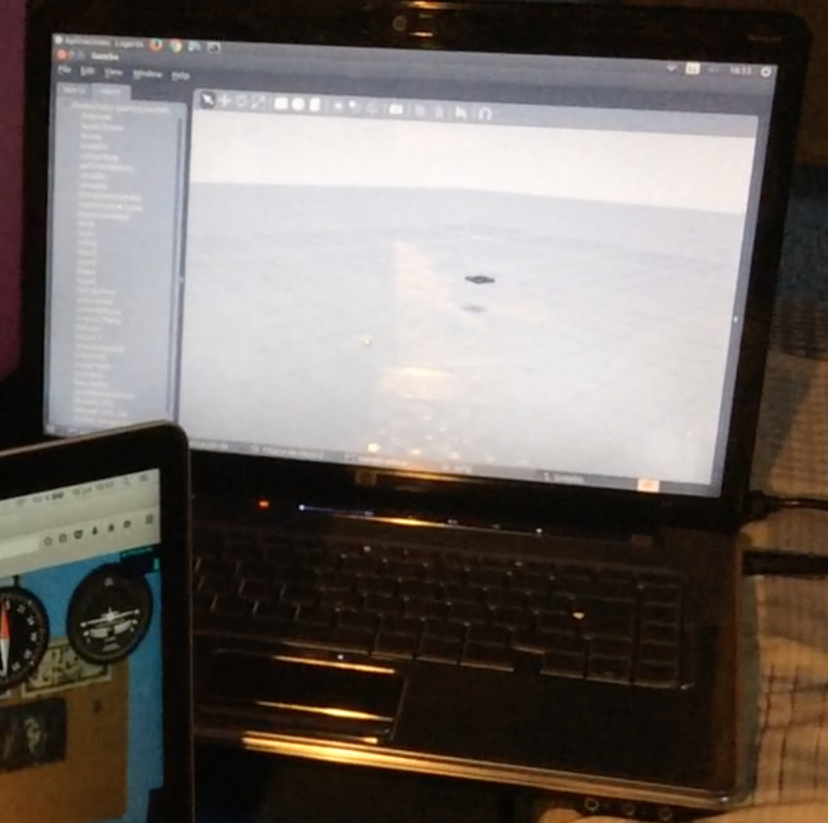
\includegraphics[width=47mm]{sec_exp1_2}
  \end{subfigure}
    \hspace{0.5pt}
    \begin{subfigure}[]{47mm}
    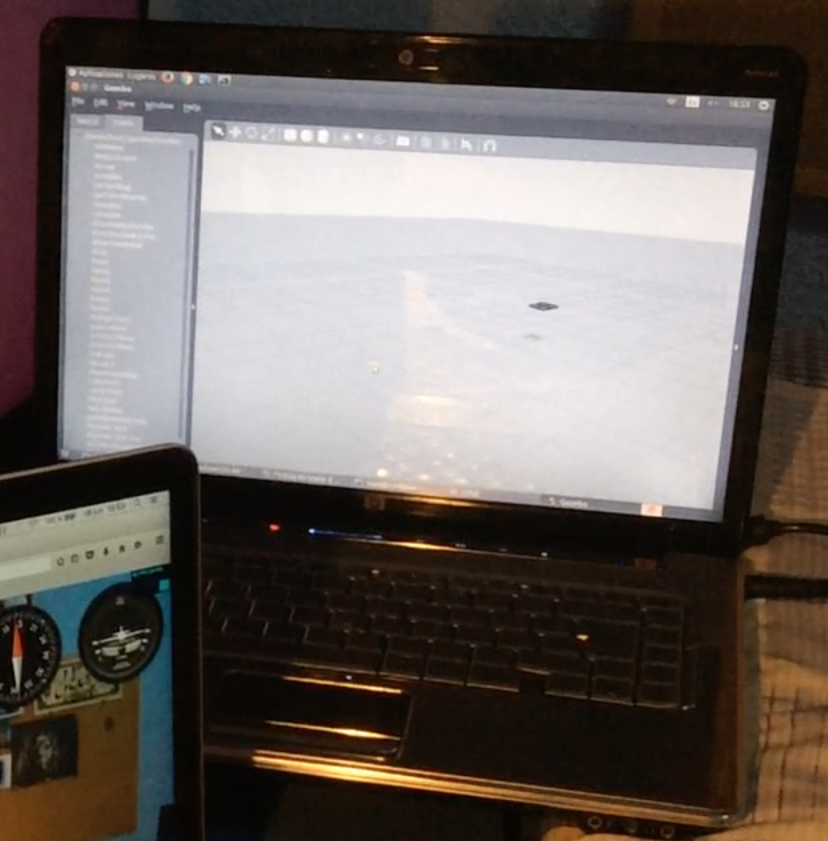
\includegraphics[width=47mm]{sec_exp1_3}
  \end{subfigure}
    \caption{Secuencia de movimiento del drone dentro de Gazebo.}
  \label{fig:secexp1}
\end{figure}


\section{Vuelo del drone real}

Las pruebas con el drone real se han divido a su vez en dos. La primera consiste en realizar las pruebas sin colocar a bordo del drone ni el \emph{computer stick} ni la cámara. Ambos se han usado para las pruebas pero para una primera aproximación se han realizado sin estar a bordo.\\

\begin{figure}[h!]
\centering
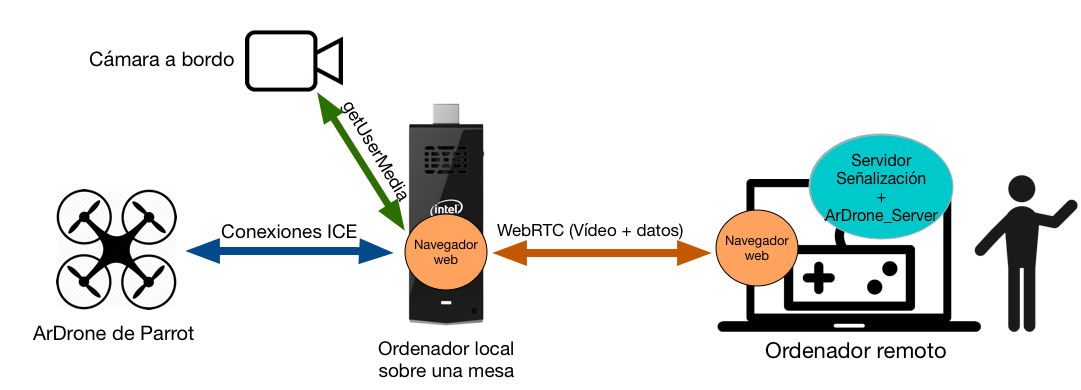
\includegraphics[width=0.9\textwidth]{esquema_experimento2}
\caption{Esquema del experimento con el drone real.}
\label{fig:esquemaexperimento2}
\end{figure}

Así pues la distribución de los equipos es como se muestra en la figura \ref{fig:esquemaexperimento2}: computer stick como par local, que se conecta al drone real y accede a la cámara USB conectada al mismo, y ordenador portátil como par remoto desde el que se teleoperará el drone y a su vez está ejecutando el servidor de señalización y el \texttt{ardrone\_server.}\\

La figura \ref{fig:experimentodronereal1} muestra la realización de este experimento. En la mediawiki\footnote{\url{http://jderobot.org/Irodmar-tfg\#First\_Flying\_with\_Real\_Drone}}\cite{Mediawiki} hay un vídeo completo del mismo. En la figura \ref{fig:secexp2} se ha representado con tres imágenes la secuencia de vuelo del drone durante el experimento.\\

\begin{figure}[h!]
\centering
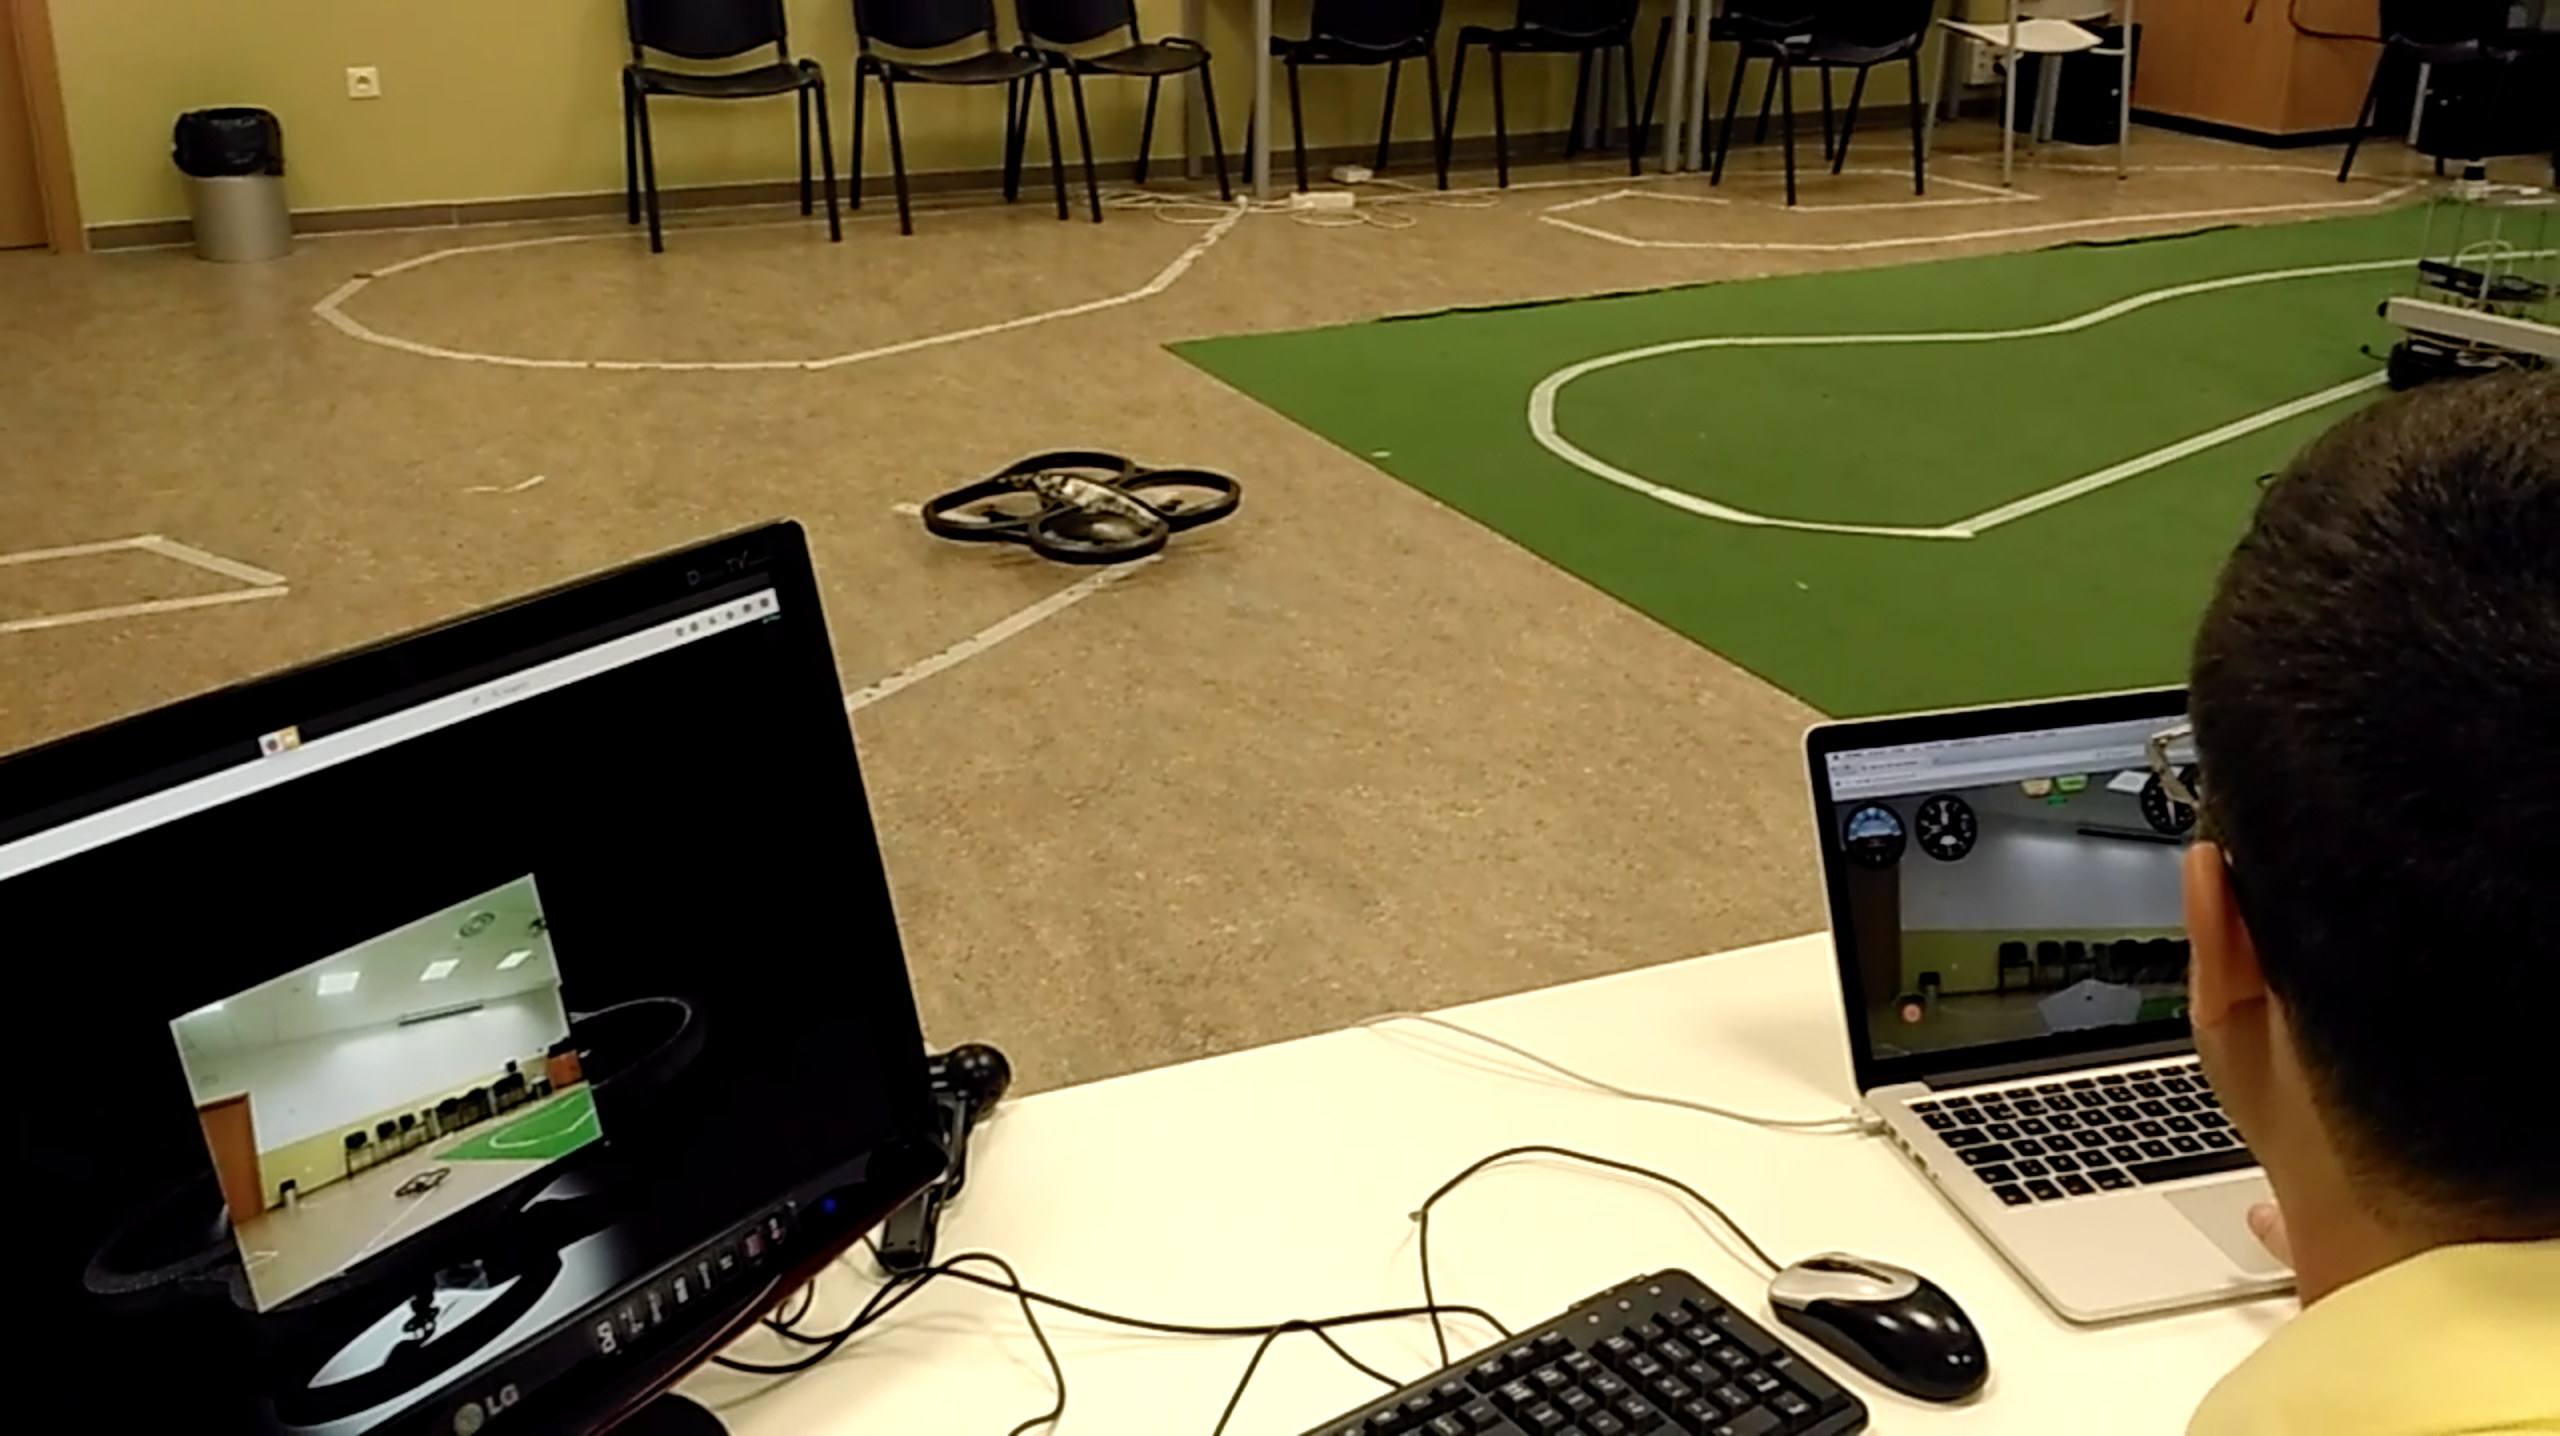
\includegraphics[width=0.9\textwidth]{experimentodronereal1}
\caption{Experimento uno con drone real.}
\label{fig:experimentodronereal1}
\end{figure}


\begin{figure}[h!]
\centering
  \begin{subfigure}[]{48mm}
    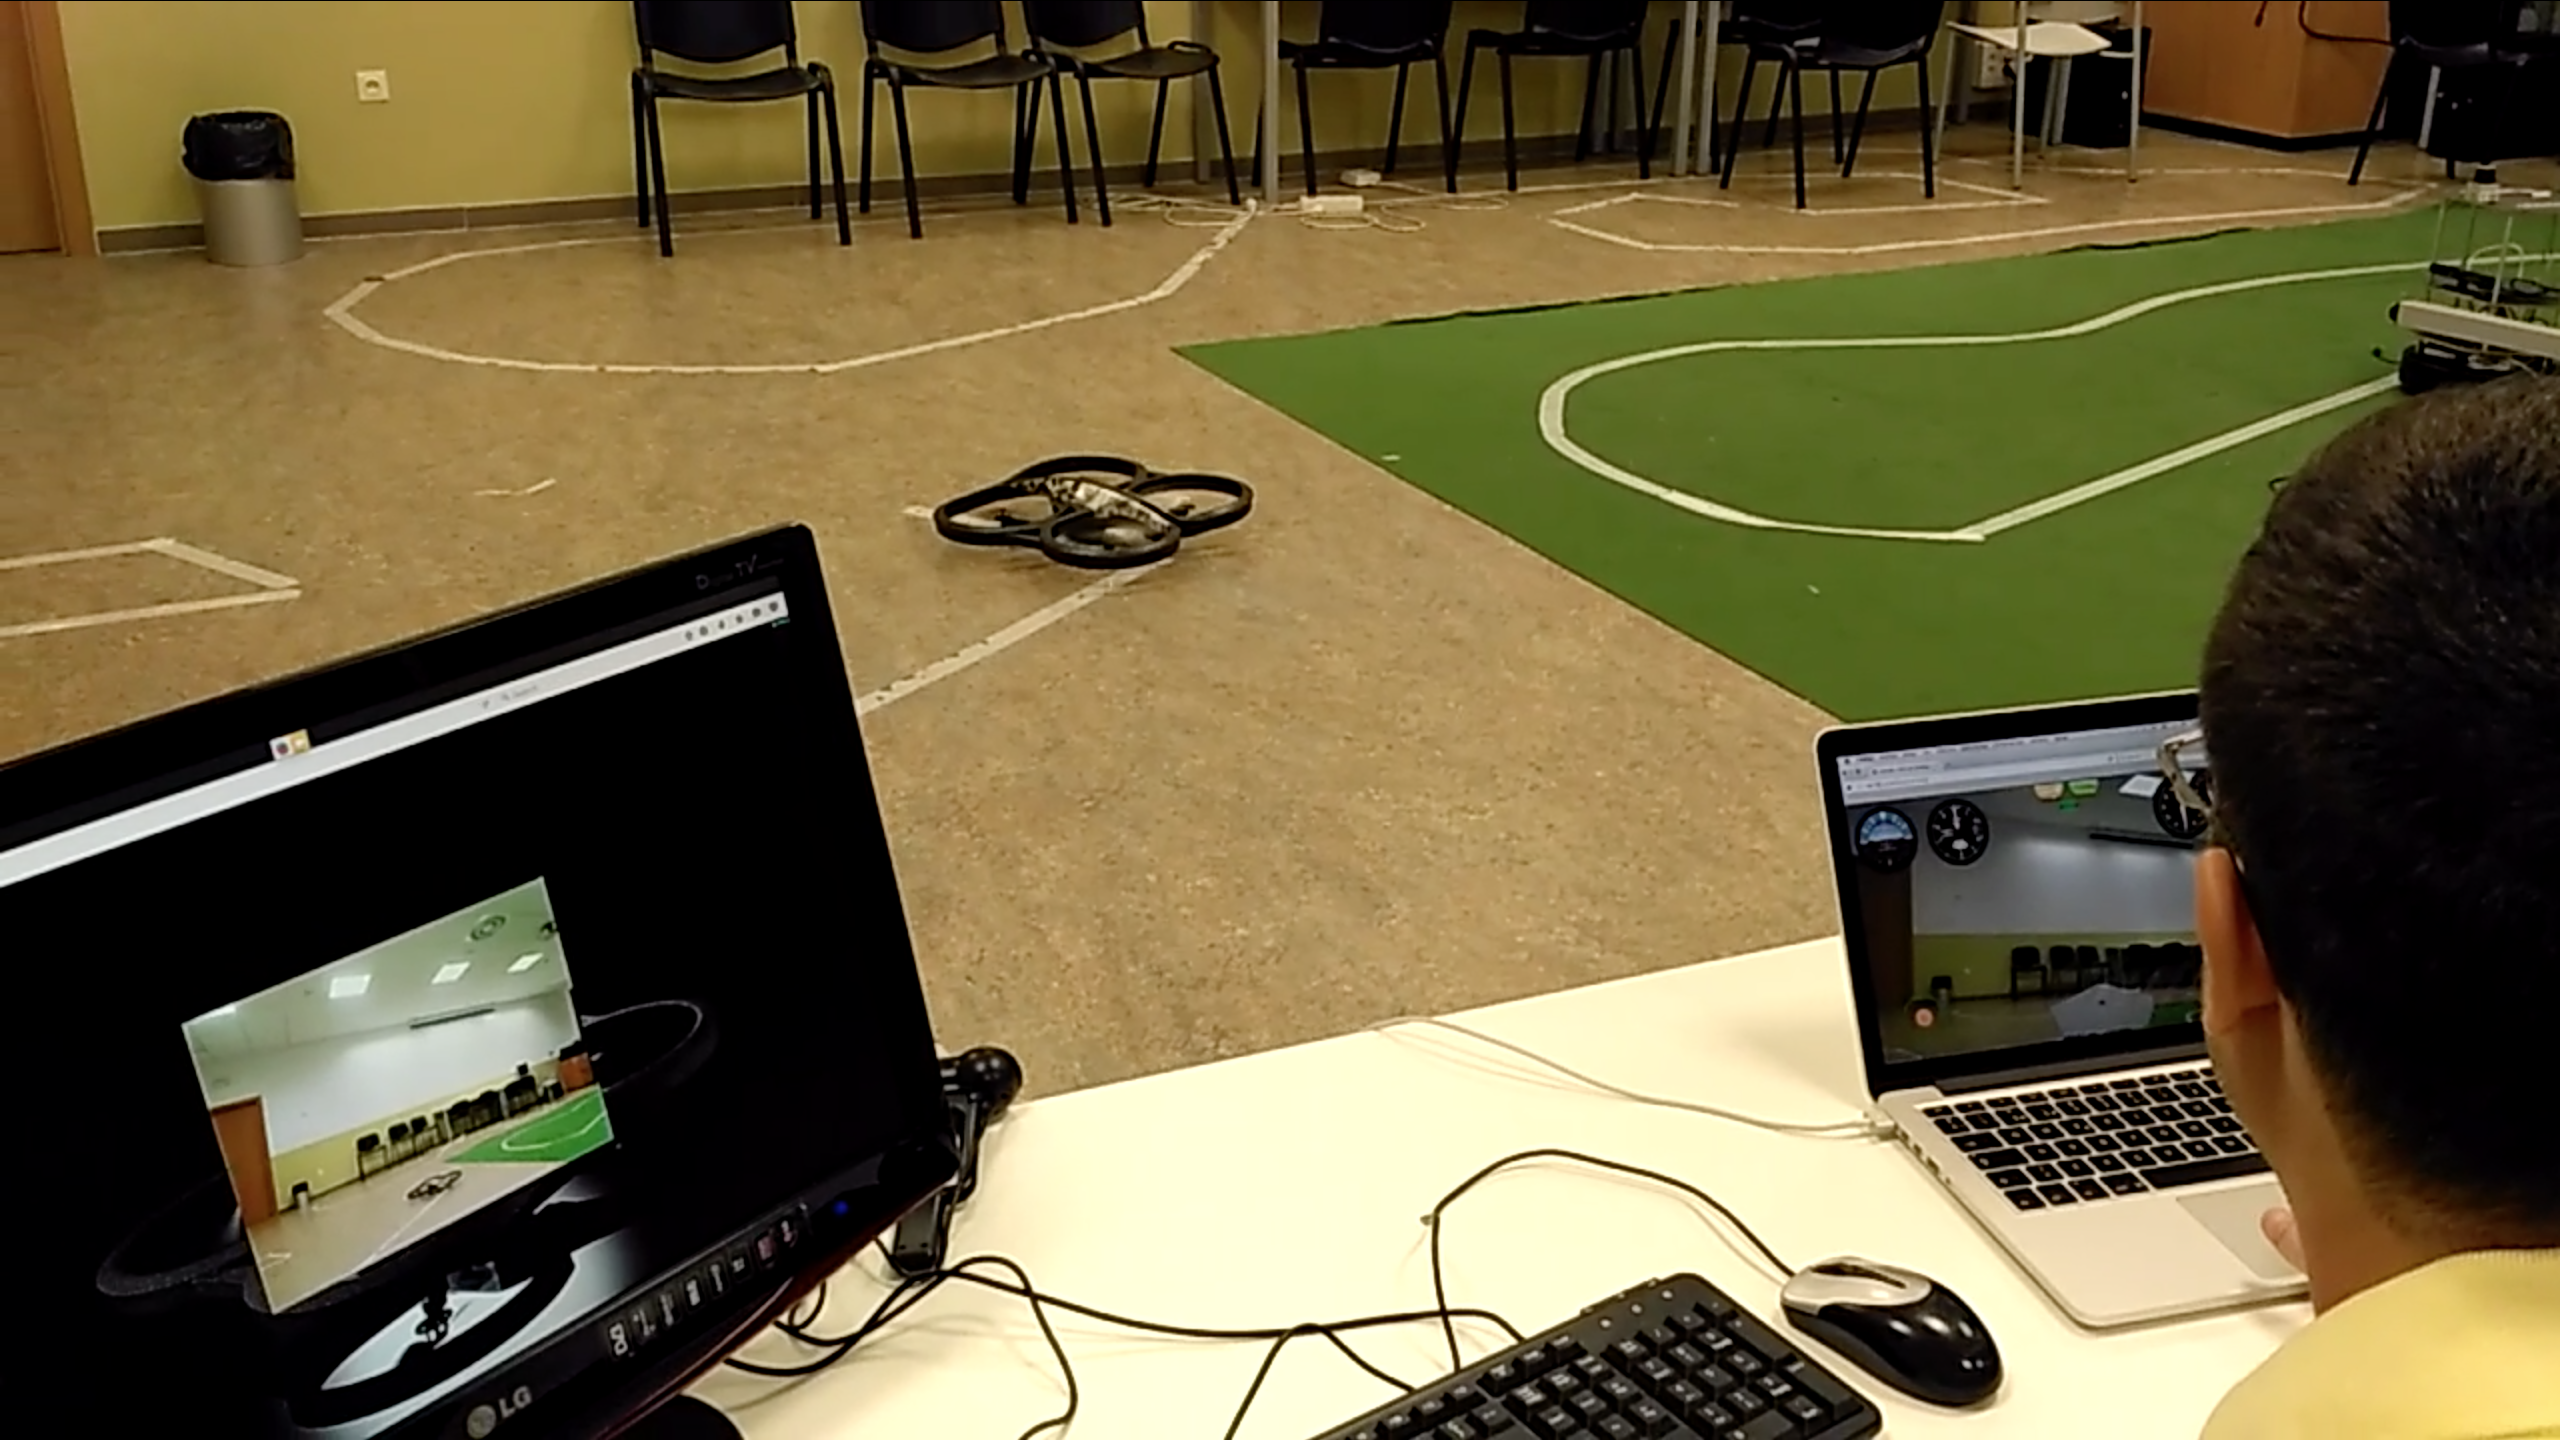
\includegraphics[width=48mm]{sec_exp2_1}
  \end{subfigure}
  \hspace{1pt}
  \begin{subfigure}[]{48mm}
    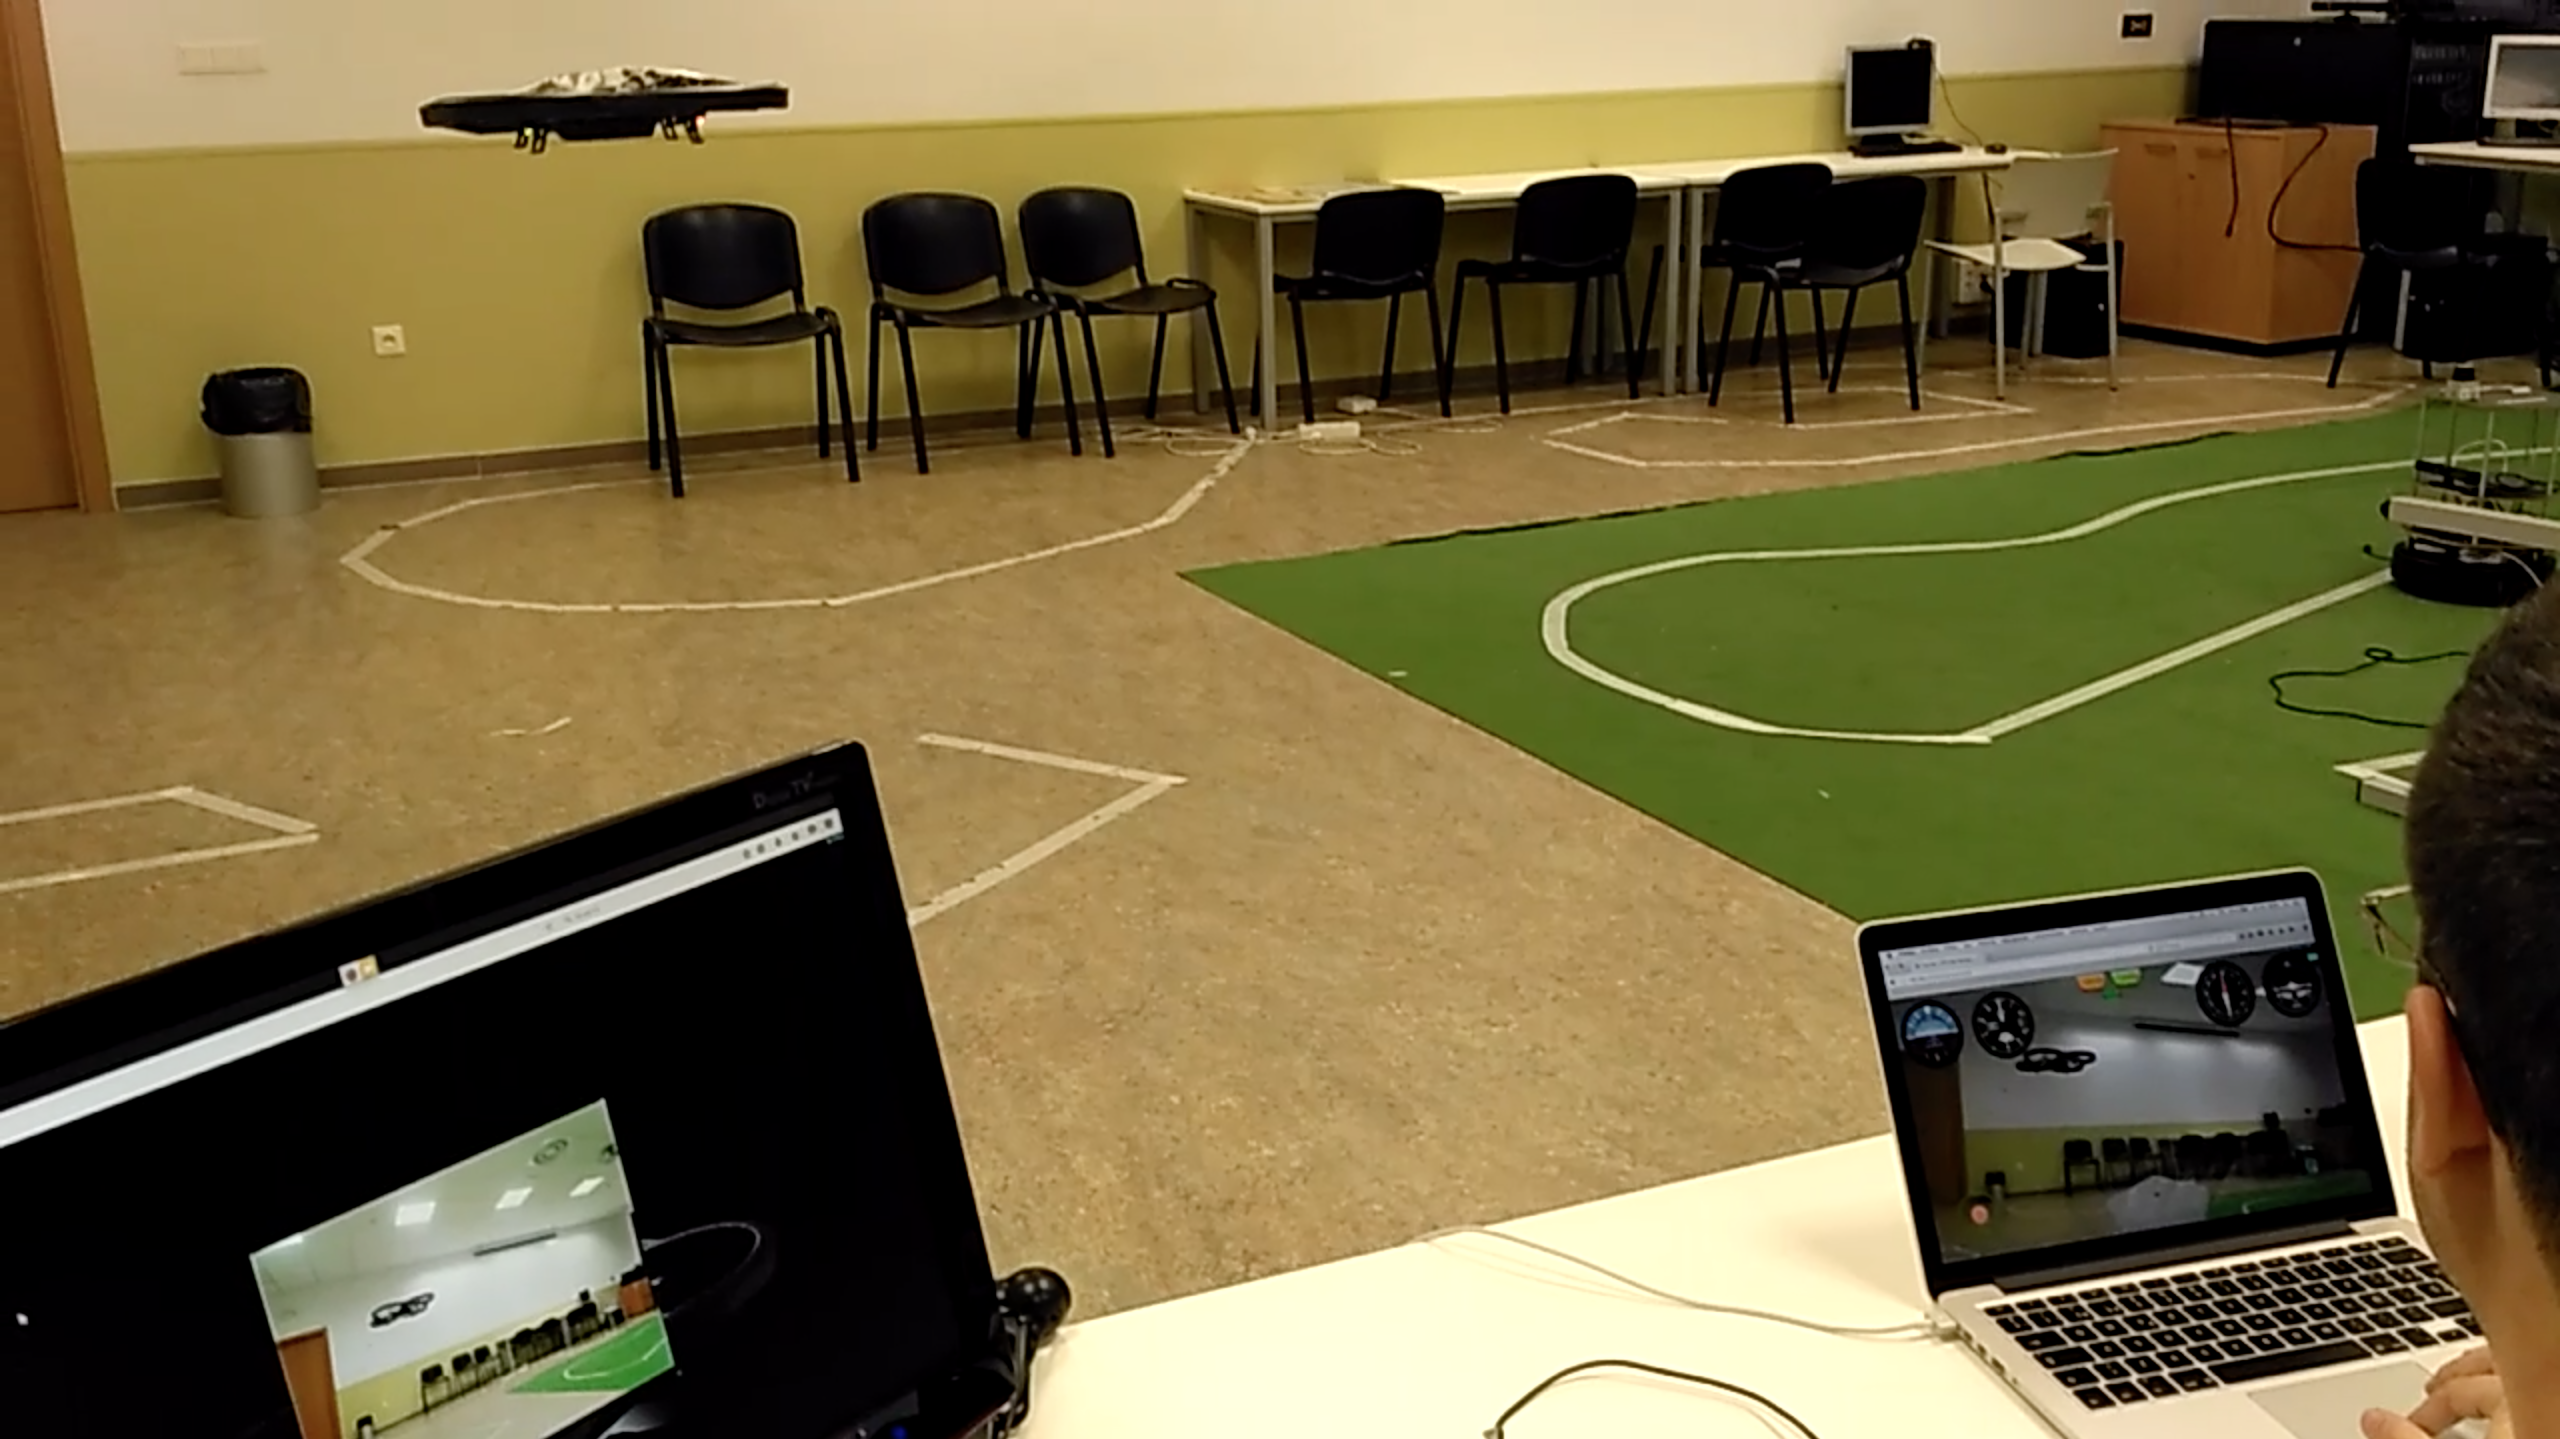
\includegraphics[width=48mm]{sec_exp2_2}
  \end{subfigure}
    \hspace{1pt}
    \begin{subfigure}[]{48mm}
    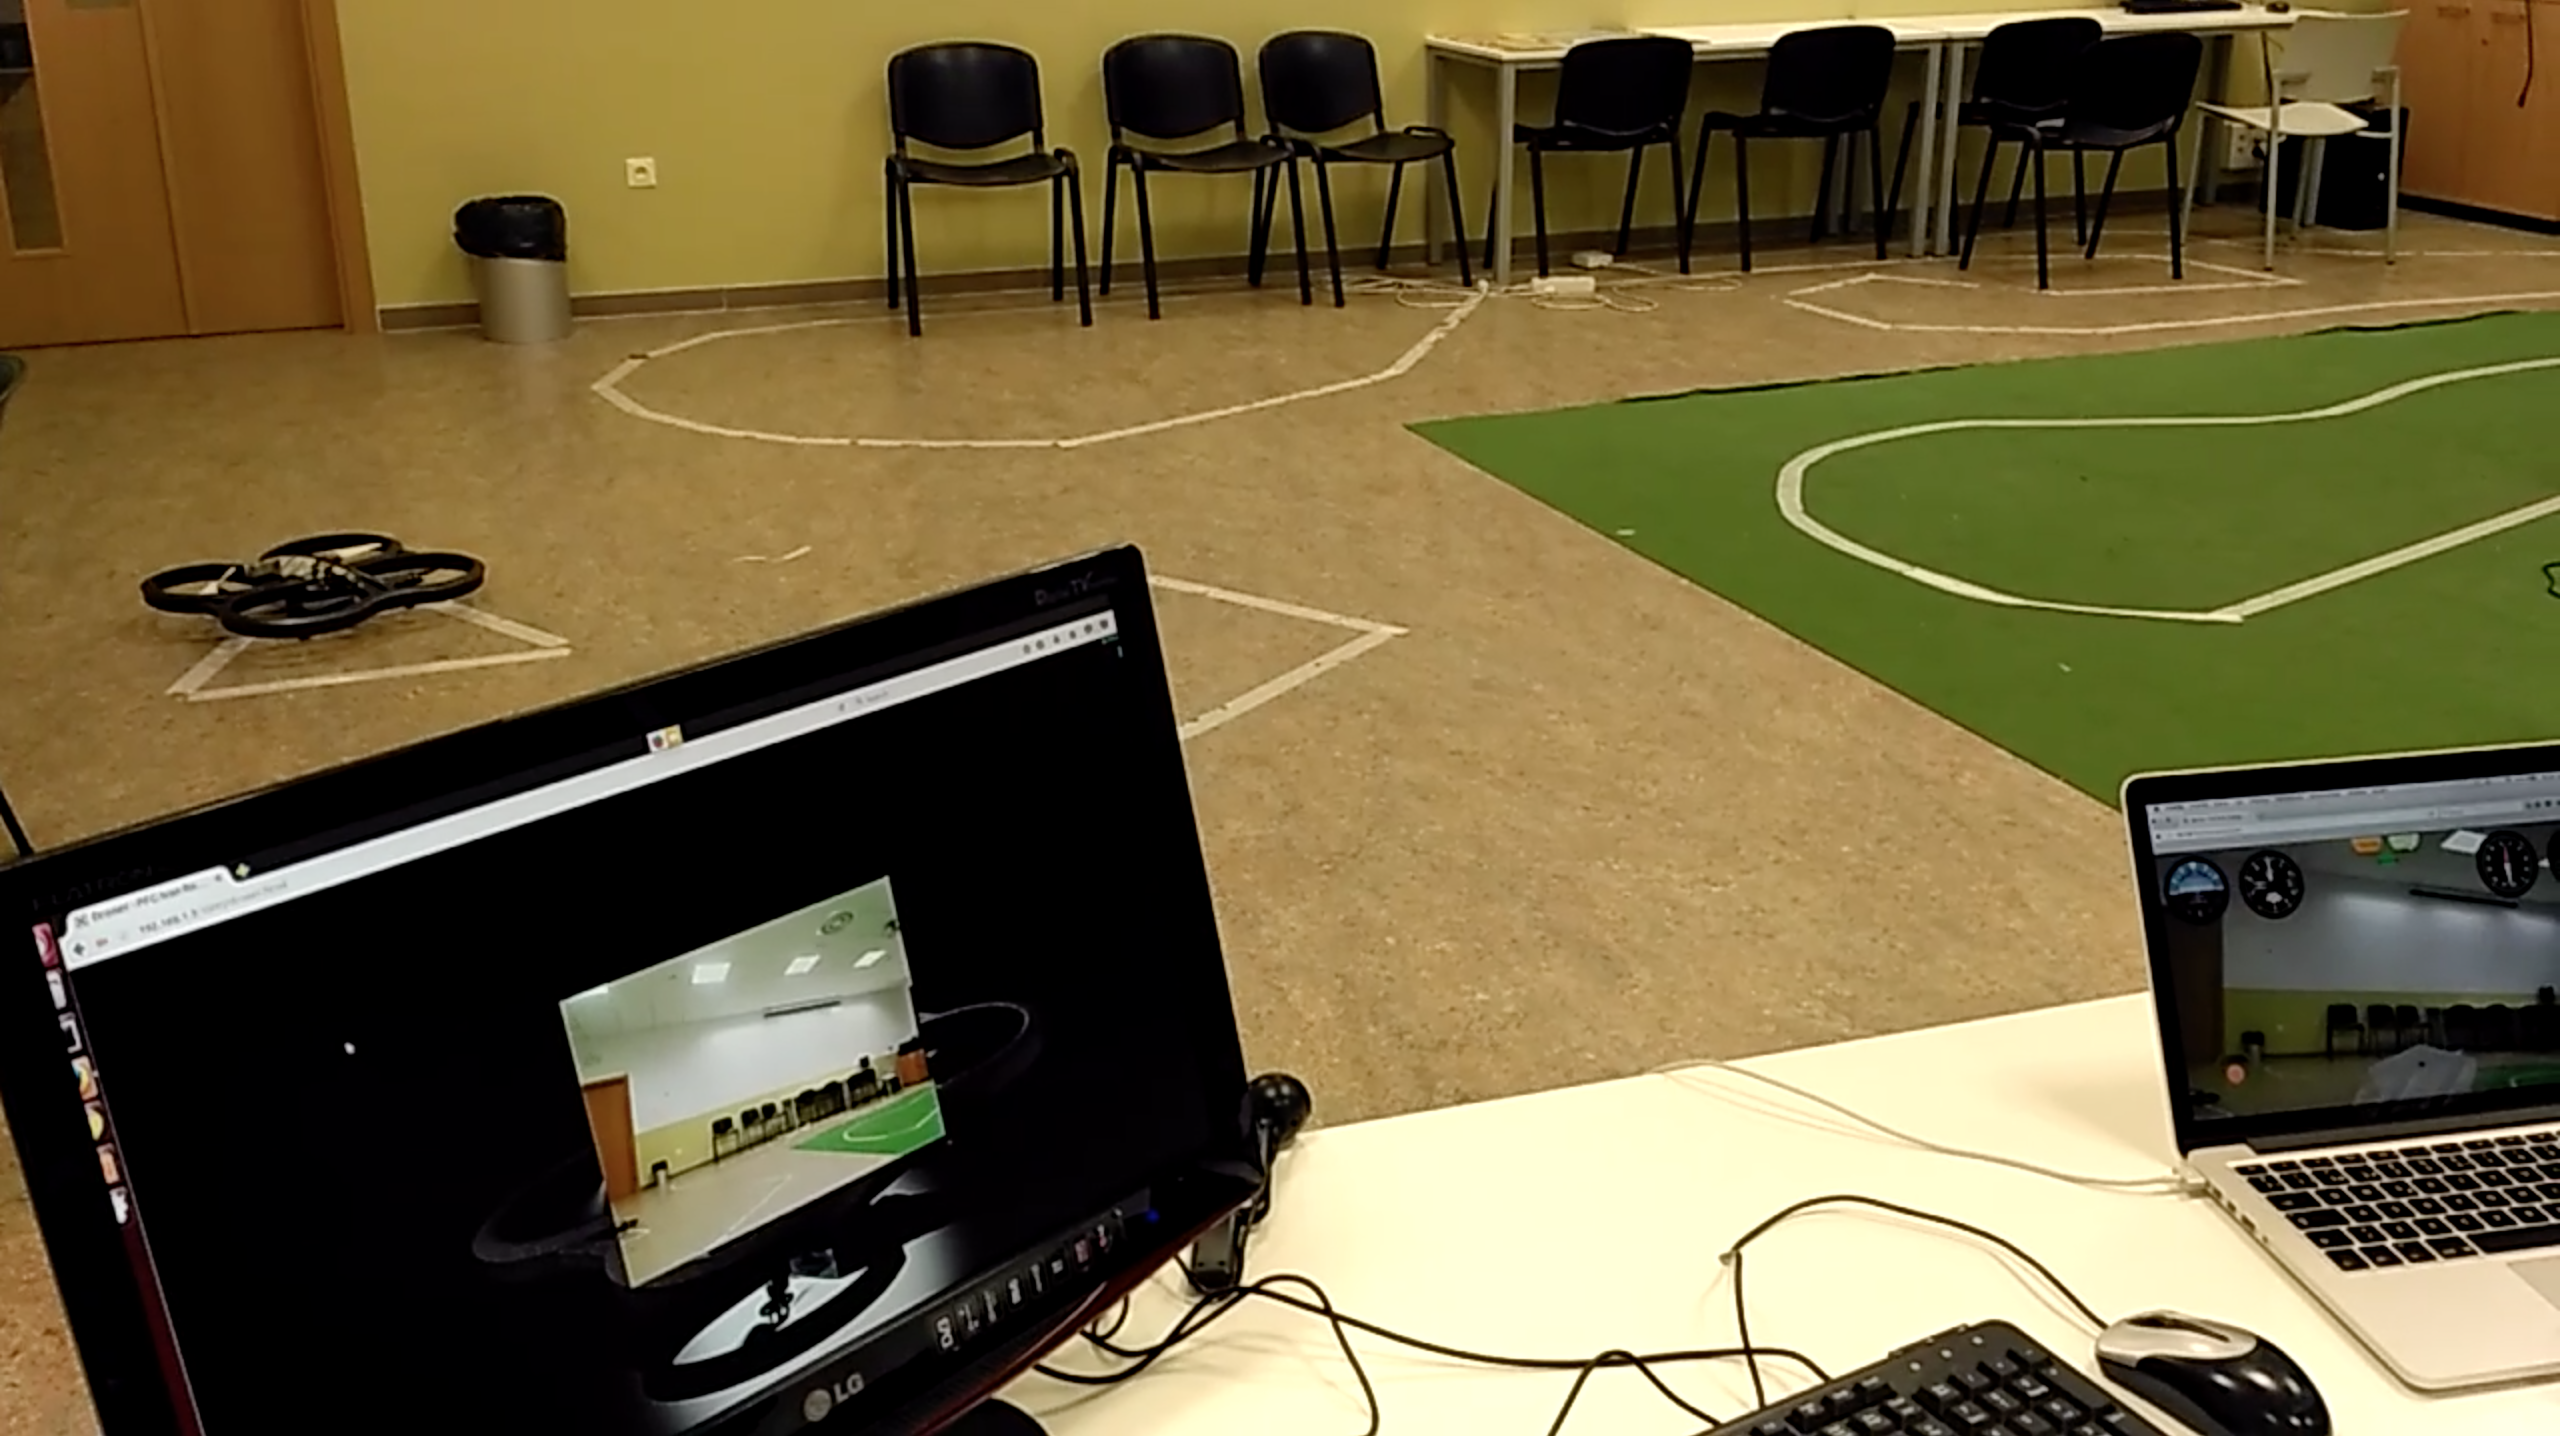
\includegraphics[width=48mm]{sec_exp2_3}
  \end{subfigure}
    \caption{Secuencia de movimiento del experimento con el drone real.}
  \label{fig:secexp2}
\end{figure}


Esta prueba también ha sido un éxito, por lo que nos marcamos el siguiente experimento con el \emph{computer stick} y la cámara a bordo del drone. Este experimento la configuración es la misma que en el anterior, pero el manejo del drone con la aplicación será más realista ya que tenemos la cámara en primera persona.\\


La segunda prueba realizada ha consistido en colocar a bordo del drone la cámara, el \emph{computer stick}, el cuál actuará como par local, estableciendo la conexión con el drone y accediendo a la cámara. El drone tiene una conexion USB de salida pero la potencia no es suficiente para hacer funcionar el \emph{computer stick}. Por este motivo se ha tenido que colocar a bordo una pila adicional la cual hará las veces de fuente de alimentación. Por otro lado tenemos un ordenador el cuál actúa como par remoto desde el que teleoperaremos el drone y además se ha utilizado para ejecutar tanto el servidor de señalización como el servidor \emph{ardrone\_server}. La figura \ref{fig:esquemaexperimentoabordo} muestra el esquema de la configuración del experimento.\\


\begin{figure}[h!]
\centering
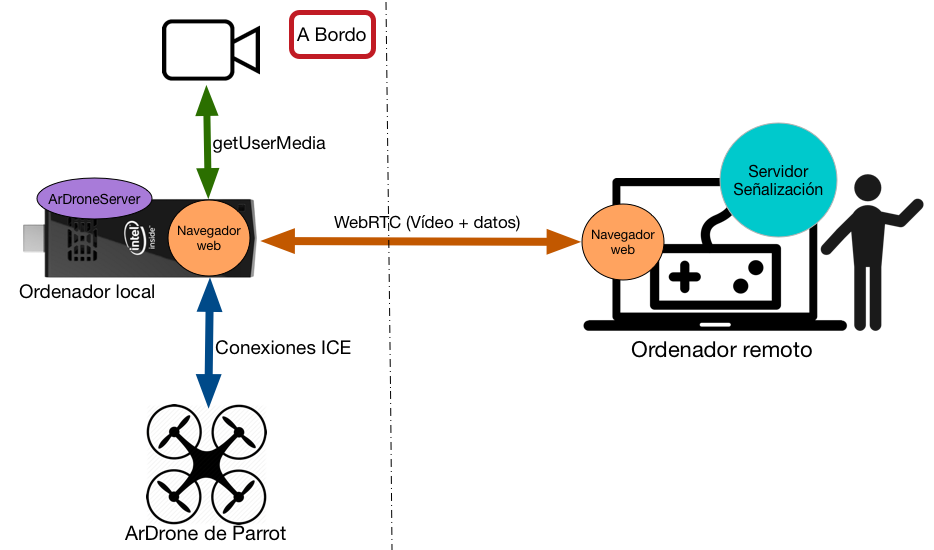
\includegraphics[width=0.7\textwidth]{esquema_experimento_abordo}
\caption{Esquema de la configuración del experimento.}
\label{fig:esquemaexperimentoabordo}
\end{figure}


En la figura \ref{fig:elementosabordo} se muestra la configuración de todos los elementos que hemos colocado a bordo del drone. Como se puede observar también hemos incluido un hub USB ya que es necesario al disponer el \emph{computer stick} de un único puerto USB y necesitar al menos dos, uno para la cámara y otro para el ratón en el momento que configuramos el navegador. Puede ver el montaje final en este vídeo\footnote{\url{http://jderobot.org/Irodmar-tfg#Experiment_Setup}} de la mediawiki.\\

\begin{figure}[h!]
\centering
\includegraphics[width=0.8\textwidth]{elementos_abordo}
\caption{Configuración de los elementos a bordo del drone.}
\label{fig:elementosabordo}
\end{figure}


Este experimento ha sido fallido, únicamente por las capacidades de vuelo que nos ofrece el drone. Entre los dispositivos que hemos colocado a bordo superamos la carga máxima de pago que permite este cuadricóptero. En lo que al funcionamiento de la aplicación se refiere ha funcionado perfectamente ya que en el par remoto obteníamos las imágenes y datos de vuelo procedentes del drone, y al ejecutar la orden de despegue el cuadricóptero ha intentado levantar el vuelo sin conseguirlo.\\

\begin{figure}[h!]
\centering
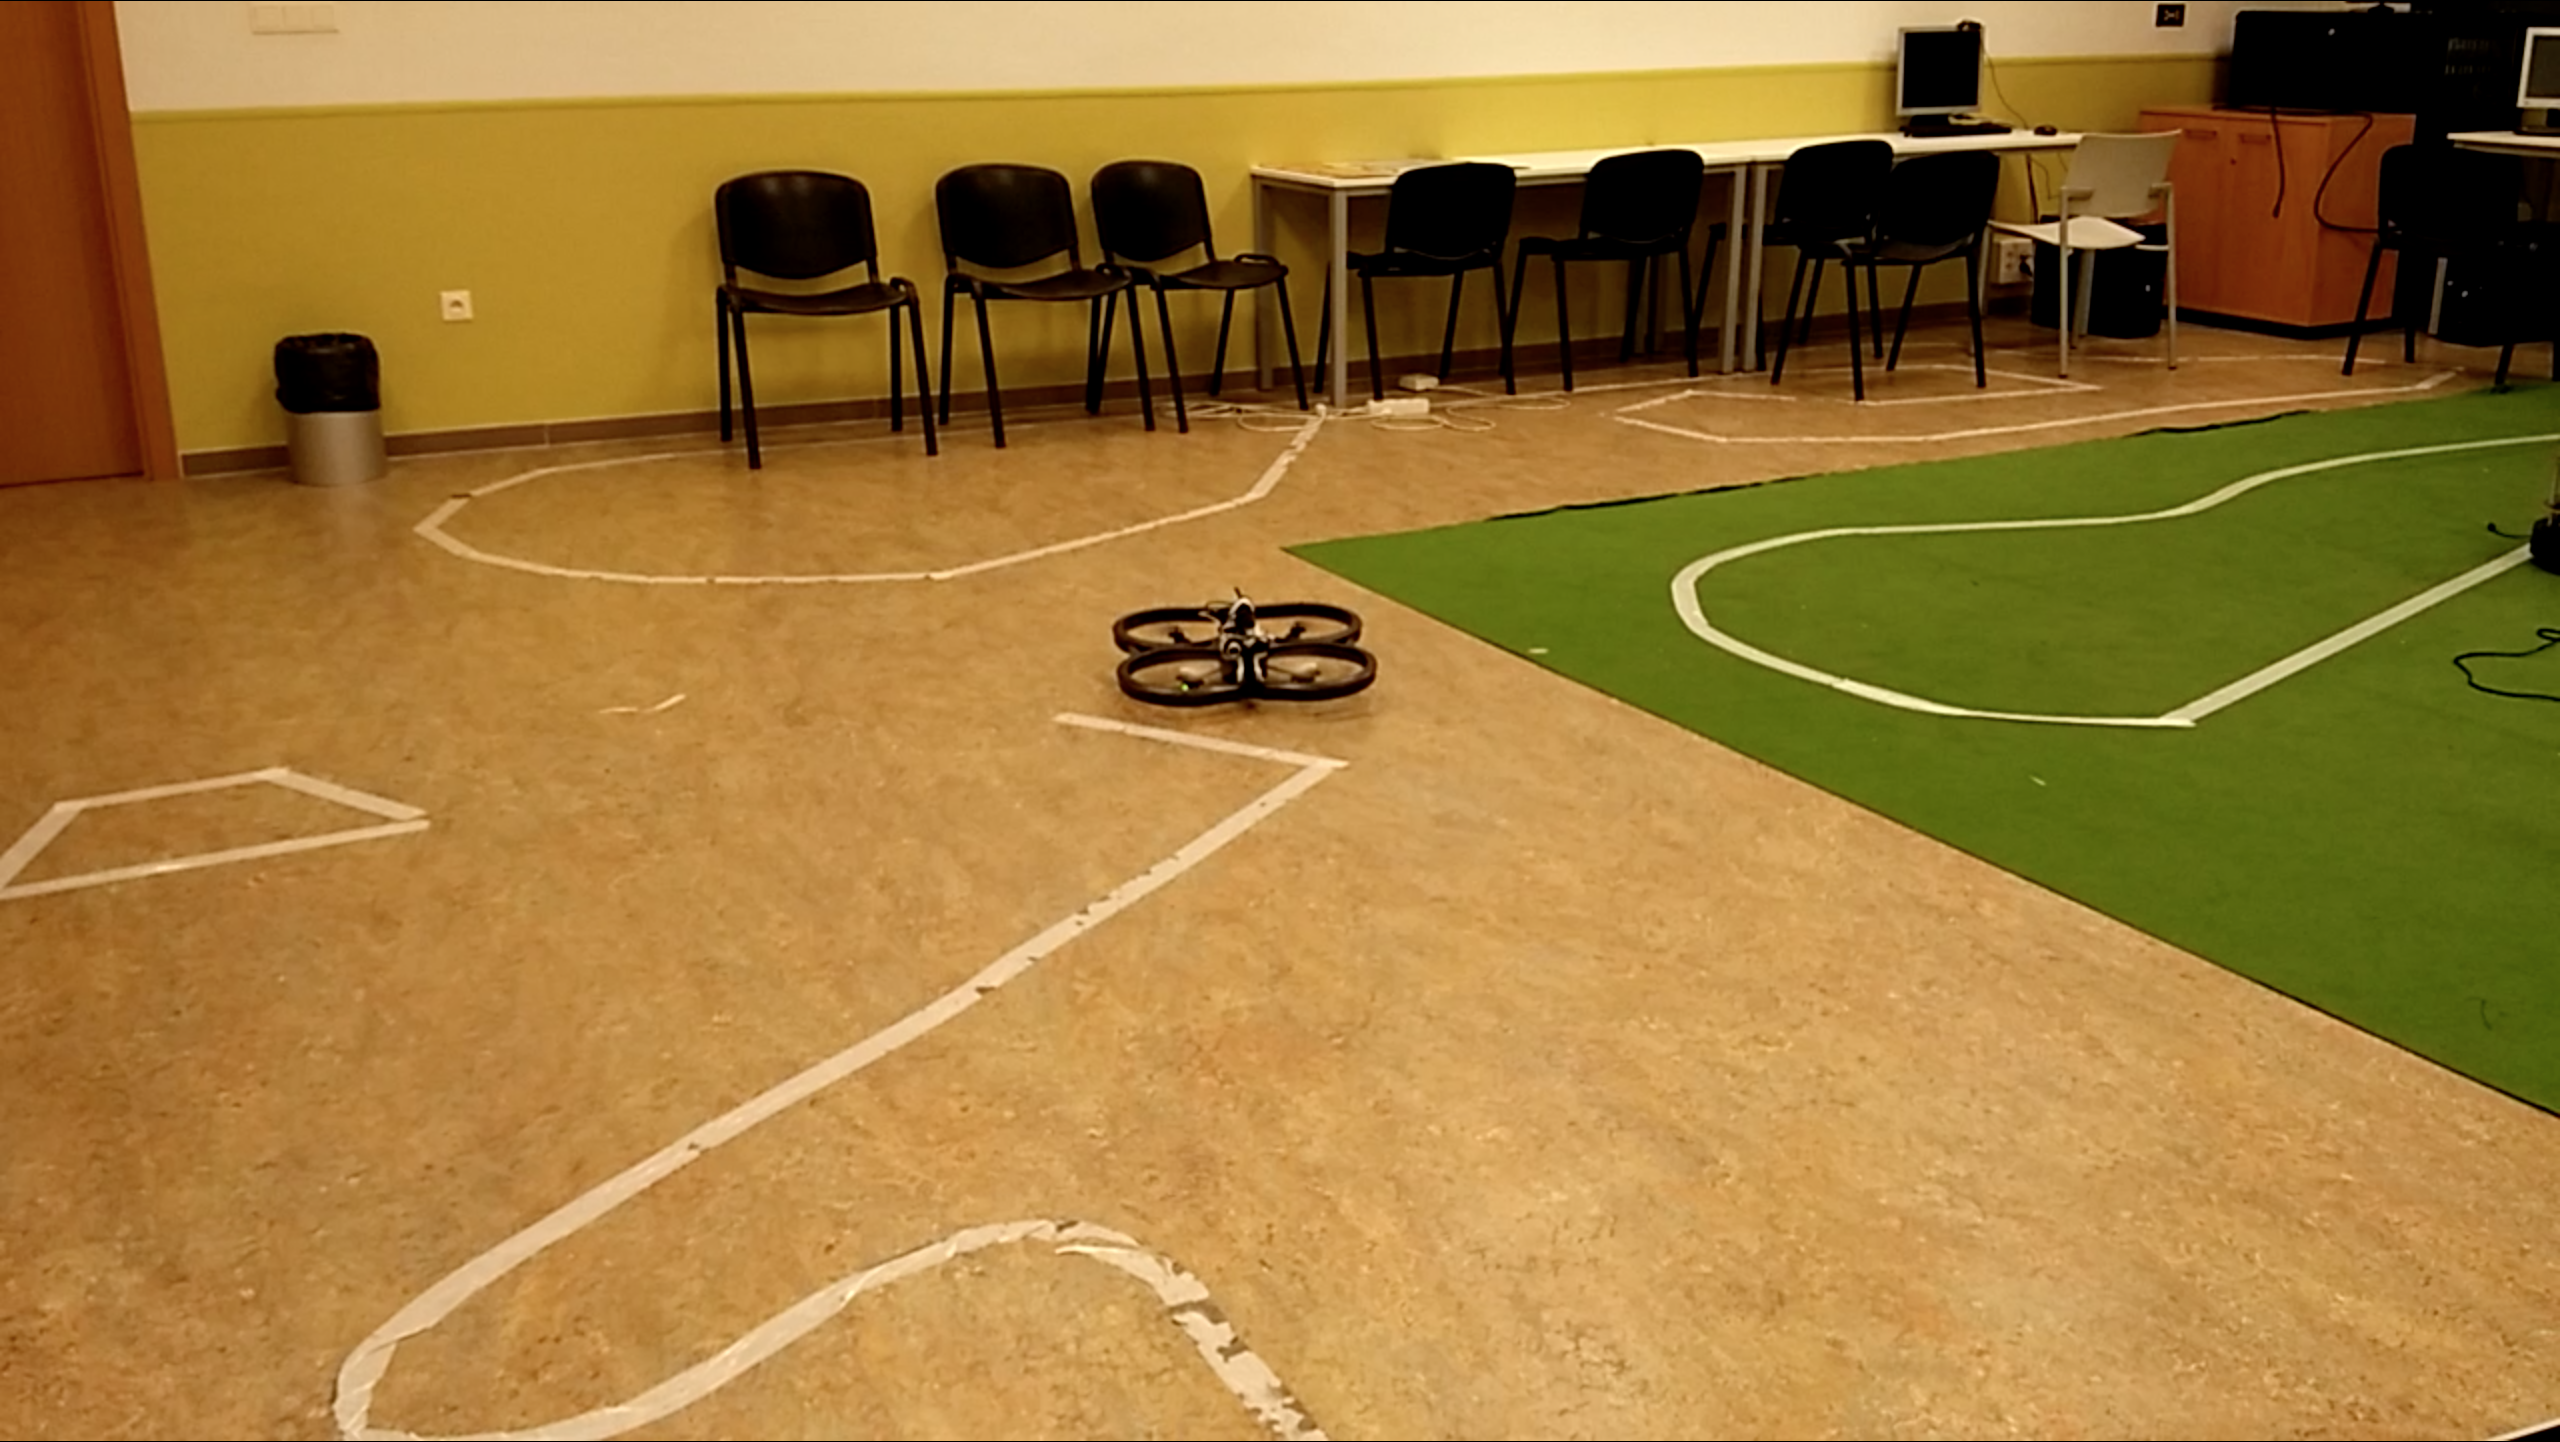
\includegraphics[width=0.7\textwidth]{experimento_abordo}
\caption{ArDrone no levanta el vuelo por exceso de peso.}
\label{fig:experimentoabordo}
\end{figure}

La figura \ref{fig:experimentoabordo} es un fotográma del vídeo\footnote{\url{http://jderobot.org/Irodmar-tfg#Attemp_of_flying}} que se grabó durante el experimento. En ella se ve al drone intentando levantar el vuelo. Para comprobar que el desarrollo funciona se optó por realizar otra prueba de vuelo en la que se cogía con las manos el drone y se le movía para observar que tanto la cámara a bordo cómo los relojes de vuelo variaban en el navegador remoto. La figura \ref{fig:pruebaexperimentoabordo} muestra un fotograma del vídeo\footnote{\url{http://jderobot.org/Irodmar-tfg#Testing_the_development}} en el que se realizan estas comprobaciones.\\

\begin{figure}[h!]
\centering
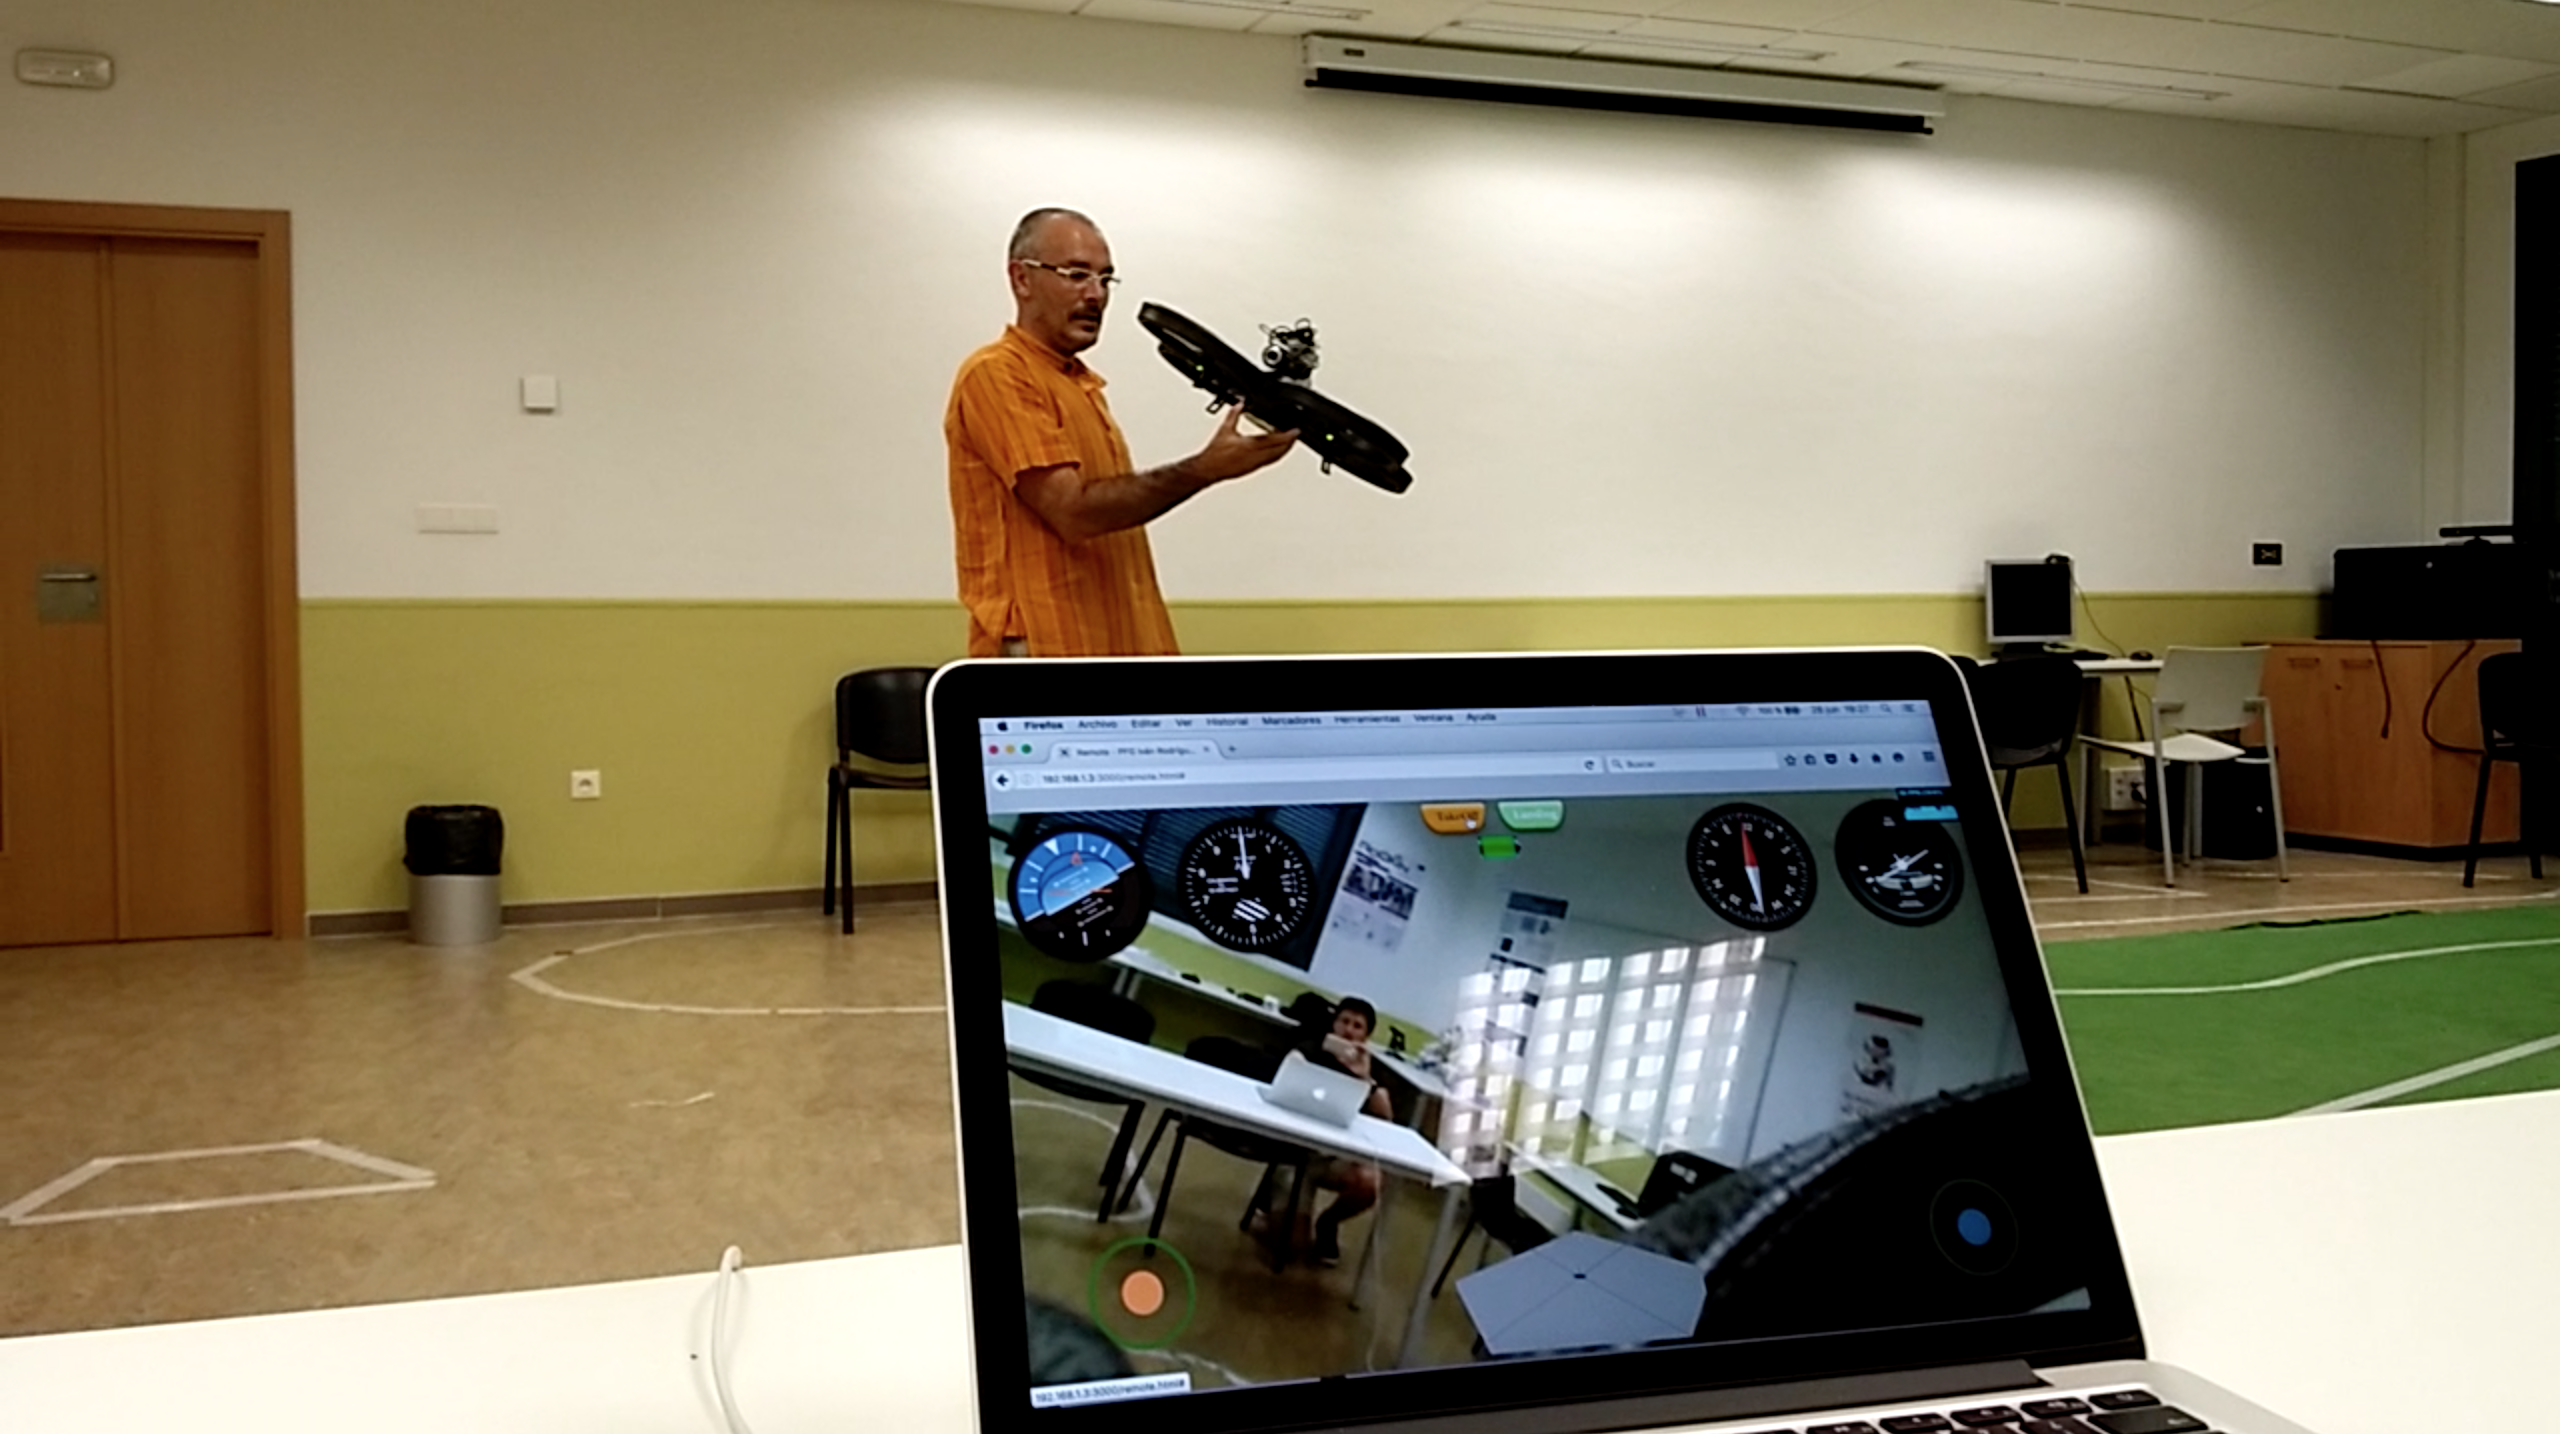
\includegraphics[width=0.7\textwidth]{pruebas_experimento_abordo}
\caption{Comprobación del funcionamiento de la aplicación.}
\label{fig:pruebaexperimentoabordo}
\end{figure}

\section{Vuelos con multidispositivos}

Como tercer y último experimento hemos probado a volar el drone utilizando dispositivos móviles. WebRTC tiene soporte para dispositivos móviles y los elementos de control los hemos desarrollado también para dispositivos táctiles, podemos utilizarlos como par remoto, par local o ambos. Al igual que el experimento anterior se ha realizado en dos pasos. Primero sin colocar el dispositivo a bordo del drone para confirmar su correcto funcionamiento y posteriormente repitiéndolo con el dispositivo a bordo. Realizar experimentos con dispositivos móviles implica la necesidad de la utilización de un ordenador de apoyo que será el que ejecute tanto el servidor de señalización para WebRTC cómo \texttt{ardrone\_server}.\\


\begin{figure}[h!]
\centering
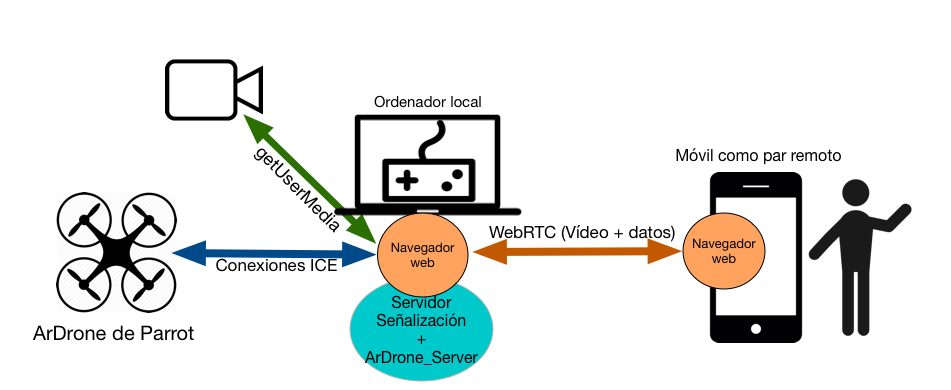
\includegraphics[width=0.8\textwidth]{esquema_experimento_multidispositivo_1}
\caption{Esquema del experimento con móvil como par remoto.}
\label{fig:esquemaexperimentomultidispositivo}
\end{figure}


Como primer experimento se ha utilizado un ordenador portátil como par local, encargado por un lado de estableciendo la conexion con el drone y de acceder a la cámara, en este caso la incorporada en el portátil, y por otro lado de correr los servidores de señalización y \texttt{ardrone\_server}. Como par remoto para teleoperar el drone se ha utilizado un teléfono móvil. En la figura \ref{fig:esquemaexperimentomultidispositivo} se detalla el esquema de este experimento.\\


En la figura \ref{fig:experimentodronemultidispositivo1} se puede apreciar un instante del experimento cuyo vídeo se encuentra en la mediawiki\footnote{\url{http://jderobot.org/Irodmar-tfg\#Flying\_with\_a\_mobile\_like\_Remote\_PC}}. En la figura \ref{fig:secexp3} podemos ver la secuencia de movimiento del drone teleoperado con un dispositivo móvil.\\

\begin{figure}[h!]
\centering
\includegraphics[width=0.9\textwidth]{experimentodronemultidispositivo1}
\caption{Experimento con móvil como par remoto.}
\label{fig:experimentodronemultidispositivo1}
\end{figure}


\begin{figure}[h!]
\centering
  \begin{subfigure}[]{48mm}
    \includegraphics[width=48mm]{sec_exp3_1}
  \end{subfigure}
  \hspace{1pt}
  \begin{subfigure}[]{48mm}
    \includegraphics[width=48mm]{sec_exp3_2}
  \end{subfigure}
    \hspace{1pt}
    \begin{subfigure}[]{48mm}
    \includegraphics[width=48mm]{sec_exp3_3}
  \end{subfigure}
    \caption{Secuencia de movimiento del experimento con dispositivo móvil como par remoto.}
  \label{fig:secexp3}
\end{figure}


\newpage
El segundo experimento (figura \ref{fig:esquemaexperimentomultidispositivo2}) es a la inversa, se utiliza un ordenador portátil como par remoto y un teléfono móvil como par local.

\begin{figure}[h!]
\centering
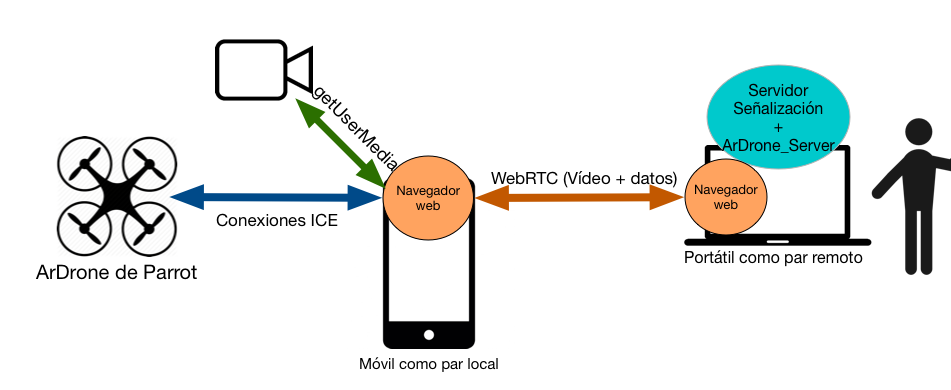
\includegraphics[width=0.8\textwidth]{experimento_multidispositivo2}
\caption{Esquema del experimento con móvil como par local.}
\label{fig:esquemaexperimentomultidispositivo2}
\end{figure}

En este configuración el ordenador portátil se utiliza también para ejecutar los servidores de señalización y \texttt{ardrone\_server}. El móvil se usa como par local, encargándose de establecer la conexion con el drone. En este caso las imágenes que se envían son de una de las dos cámaras del móvil, la delantera o la trasera, pudiendo elegir cualquiera de las dos. En este experimento el móvil lo colocamos sobre la mesa mirando hacia la posición en la que se encuentra en drone, por lo que en la pantalla del ordenador remoto le veremos moviéndose. La figura \ref{fig:experimentodronemultidispositivo2} muestra un momento del experimento que esta recogido en un vídeo en la mediawiki\footnote{\url{http://jderobot.org/Irodmar-tfg#Flying_with_a_mobile_like_Droner_PC}}. En la figura \ref{fig:secexp4} se muestra una secuencia del vuelo realizado.\\

\begin{figure}[h!]
\centering
\includegraphics[width=0.9\textwidth]{experimentodronemultidispositivo2}
\caption{Experimento con móvil como par local.}
\label{fig:experimentodronemultidispositivo2}
\end{figure}


\begin{figure}[h!]
\centering
  \begin{subfigure}[]{48mm}
    \includegraphics[width=48mm]{sec_exp4_1}
  \end{subfigure}
  \hspace{1pt}
  \begin{subfigure}[]{48mm}
    \includegraphics[width=48mm]{sec_exp4_2}
  \end{subfigure}
    \hspace{1pt}
    \begin{subfigure}[]{48mm}
    \includegraphics[width=48mm]{sec_exp4_3}
  \end{subfigure}
    \caption{Secuencia de movimiento del experimento con dispositivo móvil como par local.}
  \label{fig:secexp4}
\end{figure}

Se ha desestimado la realización del experimento en el que situamos el móvil a bordo del drone debido a la dificultad de colocarlo en posición vertical para que la cámara apunte desde la parte delantera del drone. La única posición dónde podría colocarse es en un extremo del cuadricóptero lo que causaría una descompensación de cargas dando lugar a que el drone no pudiese estabilizar el vuelo.\\


\chapter{Conclusiones}

En capítulos anteriores hemos descrito el contexto y el problema que abordamos en este proyecto, la solución propuesta junto con una serie de pruebas y experimentos que validan y software desarrollado. En este capítulo se exponen las conclusiones obtenidas y las posibles líneas por las que se puede continuar el trabajo.\\

\section{Conclusiones}

Bajo una mirada retrospectiva se puede observar que se han cumplido satisfactoriamente los objetivos generales que nos habíamos marcado. Hemos creado una aplicación web entre navegadores sin servidores intermedios que nos permite controlar, manejar y monitorizar un cuadricóptero desde un navegador, por ejemplo un teléfono móvil. Dentro de este objetivo nos marcamos tres subjetivos, los cuáles también hemos cumplido:\\

\begin{itemize}
\item Hemos creado una conexion local directamente con los sensores y actuadores del drone mediante un navegador web sin necesidad de servidores intermedios utilizando \emph{getUserMedia} de WebRTC para la cámara y ICE con \emph{WebSockets} para comunicar el navegador con el servidor JdeRobot para el drone (\texttt{ardrone\_server}).
\item Se ha desarrollado una conexión entre navegadores que transfieren en tiempo real y sin servidores intermedios la cámara y los datos necesarios para monitorar los sensores del drone y teleoperarlo. Para ello se ha utilizado \emph{RTCPeerConnection} para el vídeo y \emph{RTCDataChannel} para transmitir los datos de los sensores del drone desde el par local hacia el par remoto y en sentido opuesto las órdenes dadas por el usuario final.
\item Se ha creado una interfaz web amigable que nos permite monitorar la cámara y los sensores del drone, así como teleoperarlo de una manera muy intuitiva y sencilla de usar. Esta interfaz consta de un vídeo de fondo a pantalla completa, unos relojes de navegación dónde se representan los datos recibidos de los sensores del drone, unos \emph{joystick} virtuales para controlar el drone y un visor 3D.
\end{itemize} 

A parte de estos subobjetivos se le han añadido unos extras, como poder teleoperarlo con un mando o que tanto la conexión local como remota, así como la interfaz sean multiplataforma y multidispositivo, lo que nos permite controlarlo desde un teléfono móvil o tableta, por ejemplo.\\

Todo lo desarrollado se ha validado experimentalmente tal y como se muestra en el capítulo 5.\\

Se puede encontrar tanto esta memoria, como el repositorio del código, vídeos, explicaciones, ejemplos y resultados obtenidos en la mediawiki oficial del proyecto\footnote{\url{http://jderobot.org/Irodmar-tfg}}\cite{Mediawiki}.\\

\section{Trabajos futuros}

A todo proyecto hay que ponerle unos límites y este no es una excepción. Sirve como base y punto de partida para otros proyectos o trabajos con los que ampliar esta aplicación. Dentro de las lineas de desarrollo que se podrían seguir exponemos algunas de ellas:\\

Uno de las líneas más útiles de desarrollo podría ser incorporar diversas cámaras al drone y tener la posibilidad en el par remoto de cambiar entre ellas según nuestras necesidades.\\

Un paso más podría ser dotar al drone de autonomía, pudiendo indicarle desde el ordenador remoto unas coordenadas para que el drone se desplazase de una a otra como si de un circuito se tratase. Esto pasa por desarrollar un autopiloto dentro del cuadricóptero que le dote de capacidades de navegación autónoma.\\

Asimismo este proyecto podría integrarse en el repositorio oficial de JdeRobot\cite{jderobot_repo} desde dónde se podrá seguir trabajando en estas lineas de desarrollo o cualquier otra según las necesidades que vayan surgiendo.\\


\begin{thebibliography}{}

\bibitem{Mediawiki} Mediawiki oficial del proyecto (WebRTC en un drone) \url{http://jderobot.org/Irodmar-tfg}
\bibitem{Repositorio} Repositorio oficial del proyecto (WebRTC en un Drone) \url{https://github.com/RoboticsURJC-students/2015-tfg-irodmar} 
\bibitem{jderobot} Proyecto JdeRobot \url{http://jderobot.org/} 
\bibitem{jderobot_repo} Repositorio de JdeRobot \url{https://github.com/RoboticsURJC/JdeRobot} 
\bibitem{ArDroneServer} Mediawiki de Alberto Martín (ArDroneServer) \url{http://jderobot.org/Amartinflorido-tfg}
\bibitem{surveillance4.0} Mediawiki Daniel Castellano (Surveillance 4.0) \url{http://jderobot.org/D.castellanob-pfc} 
\bibitem{surveillance5.1} Mediawiki Edgar Barrero (Surveillance 5.1) \url{http://jderobot.org/Aerobeat-colab}
\bibitem{teleoperadoresyvisoresweb} Mediawiki Aitor Martínez \url{http://jderobot.org/Aitormf-tfg}
\bibitem{Pagina WebRTC} Página oficial de WebRTC \url{https://webrtc.org}
\bibitem{WebRTC} W3C: Borrador de la norma WebRTC \url{http://www.w3.org/TR/webrtc/}
\bibitem{WebRTC_book} Real-Time Communication with WebRTC \url{http://shop.oreilly.com/product/0636920030911.do}
\bibitem{orilley} Capítulo 18 (WebRTC) del libro \emph{High Performance Browser Networking} \url{http://chimera.labs.oreilly.com/books/1230000000545/ch18.html}
\bibitem {WebRTC experiment} WebRTC-experiment \url{https://www.webrtc-experiment.com}
\bibitem{JSEP} JSEP  \url{https://rtcweb-wg.github.io/jsep/}
\bibitem{JSEP2} Wikipedia: JSEP  \url{https://es.wikipedia.org/wiki/JSON}
\bibitem{Senalizacion1} Señalización en \emph{Mozilla Foundation} \url{https://developer.mozilla.org/es/docs/Web/API/WebRTC_API/Connectivity}
\bibitem{Senalizacion2} HTML5Rocks.com: Señalización \url{http://www.html5rocks.com/en/tutorials/webrtc/infrastructure/}
\bibitem{Senalizacion3} WebRTC-Experiment: Señalización \url{https://www.webrtc-experiment.com/docs/WebRTC-Signaling-Concepts.html}
\bibitem{WebRTC} Seguridad en WebRTC \url{https://rtcweb-wg.github.io/security-arch/}
\bibitem{SIP} Session Initiation Protocol \url{https://es.wikipedia.org/wiki/Session_Initiation_Protocol}
\bibitem{ORTC} ORTC \url{http://ortc.org/wp-content/uploads/2015/10/ortc.html}
\bibitem{jqueryflightindicator} Relojes de navegación \url{http://sebmatton.github.io/flightindicators/}
\bibitem{bateria} Repositorio batería HTML5 y CSS3 \url{http://codepen.io/jkantner/pen/QybzKL}
\bibitem{gazebo} Página oficial Gazebo \url{http://gazebosim.org/}
\bibitem{ice} Página oficial ICE  \url{http://www.zeroc.com/}
\bibitem{ice_manual}Ice 3.5.1 Documentation  \url{https://doc.zeroc.com/display/Ice35/Home}
\bibitem{slicecomp} Uso de los compiladores de Slice \url{https://doc.zeroc.com/display/Ice36/Using+the+Slice+Compilers}
\bibitem{icejs} Página de Ice for Javascript  \url{https://zeroc.com/labs/icejs/index.html}
\bibitem{icews} Websockets en ICE \url{https://zeroc.com/labs/icejs/websocket.html}
\bibitem{threejs} Página de Three.js \url{http://threejs.org/}
\bibitem{threejs_doc} Documentación de Three.js \url{http://mrdoob.github.io/three.js/docs/}
\bibitem{threejs_curso} Curso de Three.js \url{http://stemkoski.github.io/Three.js/}
\bibitem{jquery} Página de JQuery \url{https://jquery.com/}

\end{thebibliography} 



\end{document}